\newpage
\section{Results}
\label{results}

Fig.~\ref{fig:Vtagresults1} , \ref{fig:Vtagresults2} and \ref{fig:Vtagresults3} shows the 95\% CL cross section upper limits derived from
 the single and double W/Z tagged event samples. 
The predicted cross sections as a function of resonance mass for the
considered benchmark models are overlaid.
Table~\ref{table:results} shows the results of limits and also corresponding limits from 7\TeVcc data~\cite{ref_2011}.
The observed local p-values for each model are shown in Fig.~\ref{fig:Vtagresults4} , \ref{fig:Vtagresults5} , \ref{fig:Vtagresults52} and \ref{fig:Vtagresults6}.
The largest local significance for a qW(WW) signal of 2.0(1.3)$\sigma$ is found at 1.5(1.9)\TeVcc.
An estimate of the look-else-where effect to transform the local p-values into global p-values is shown in Fig.~\ref{fig:lee}.


\begin{table}[htb]
\begin{center}
\begin{tabular}{ |c|l|l|l|l| }
\hline
Process           & \multicolumn{2}{|c|}{Observed Mass Exclusion(TeV)}  & \multicolumn{2}{|c|}{Expected Mass Exclusion(TeV)} \\
\hline
                  &    8 \TeVcc            &    7 \TeVcc              &   8 \TeVcc           &  7 \TeVcc                  \\
\hline
$q* \to qW $       & $[1.00,  3.17]$	   &  $ [1.00, 2.38] $  	&  $[1.00, 2.98]$	 &   $[1.00, 2.43]$  \\
$q* \to qZ $       & $[1.00,  2.88]$	   &  $ [1.00, 2.15] $  	&  $[1.00, 2.63]$	 &   $[1.00, 2.07]$  \\
$G_{RS} \to WW $   & $[1.00,  1.23]$	   &  -			        &  $[1.00, 1.33]$	&   -	    \\
$G_{RS} \to ZZ $   & -                     &  -   	                &  -			&  -    \\
$\PWpr \to  WZ $   & $[1.00,  1.23]$, $[1.39,  1.52]$, $[1.57,  1.61]$	   &  -			&  $[1.00, 1.44]$	&   -	    \\

\hline
\end{tabular}
\end{center}
\caption{Summary of limit setting results.}
\label{table:results}
\end{table}


\begin{figure*}[h!tpb]
\begin{center}
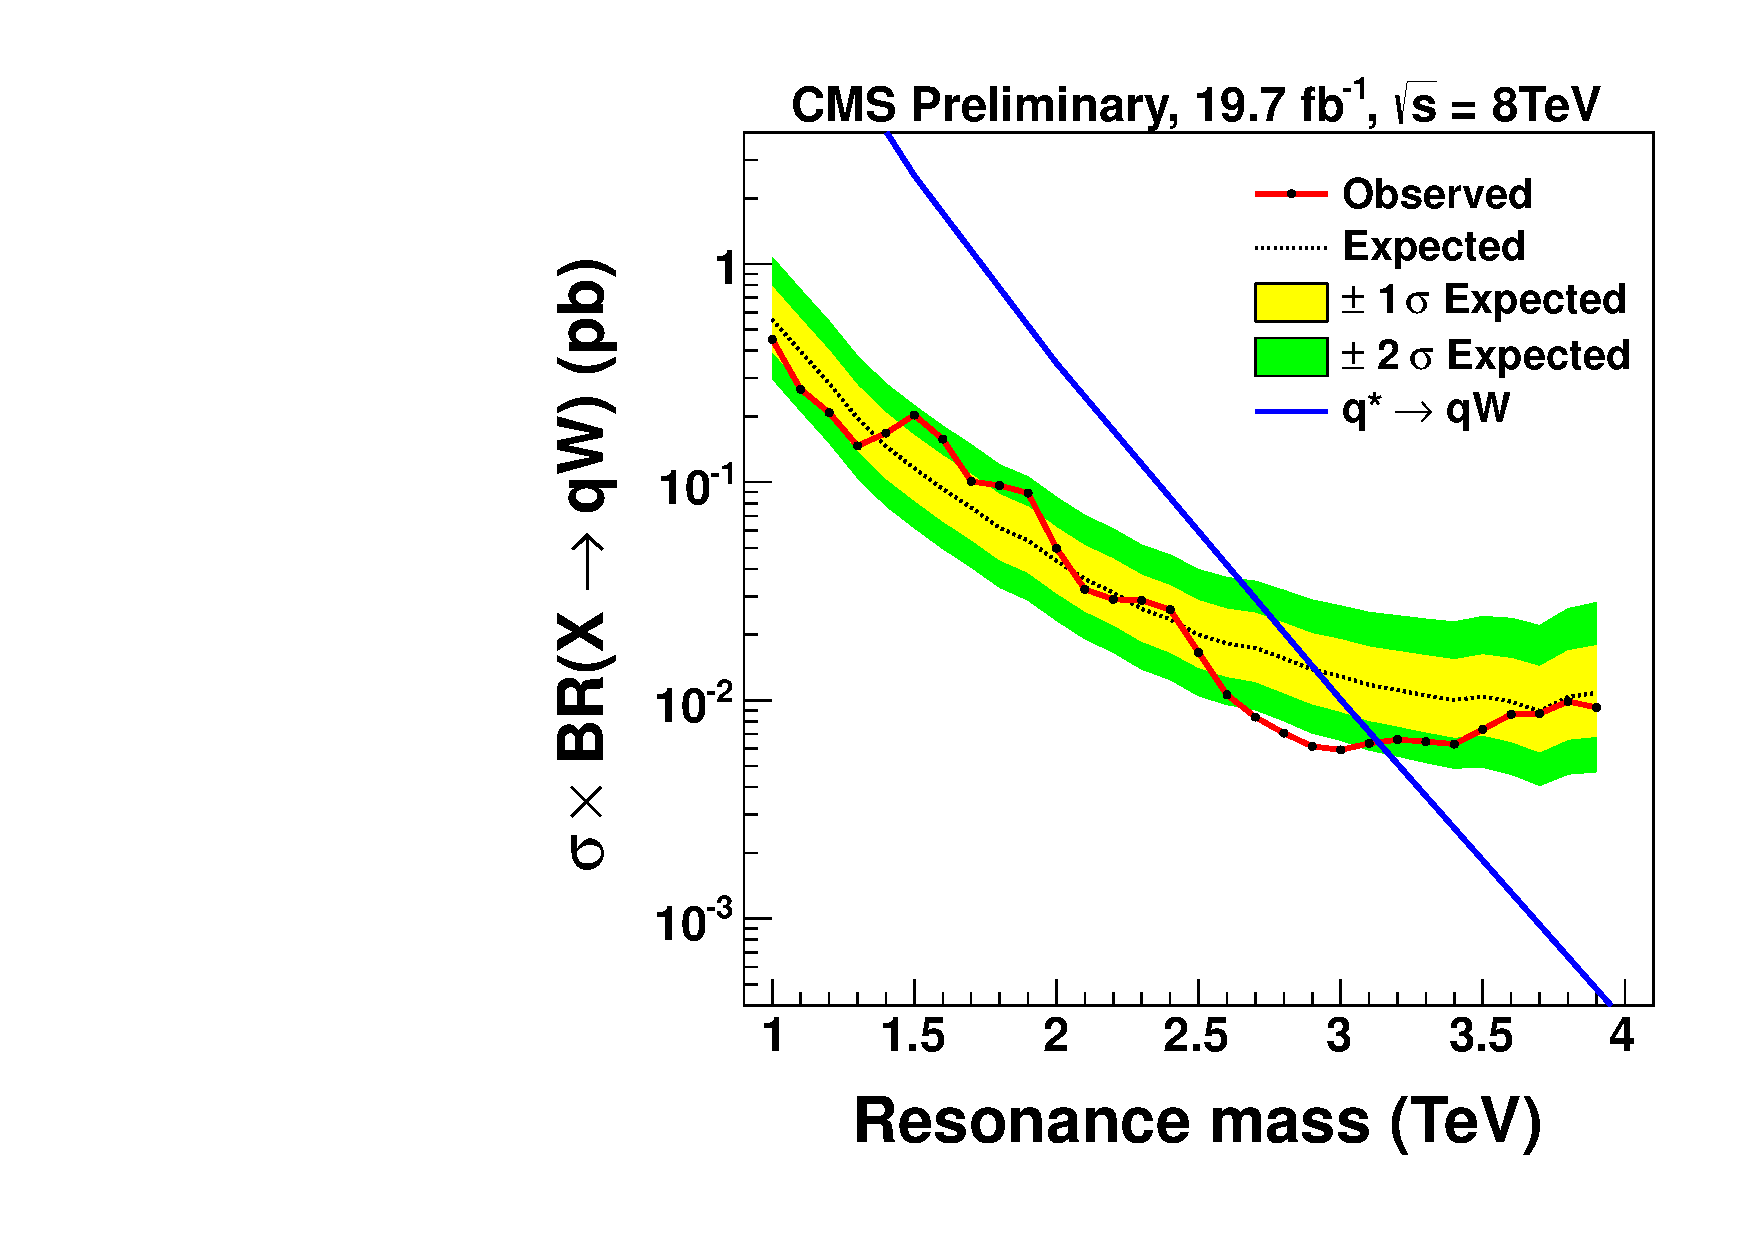
\includegraphics[width=0.35\textwidth]{figs/limits/brazilianFlag_qW_high_purity.pdf}
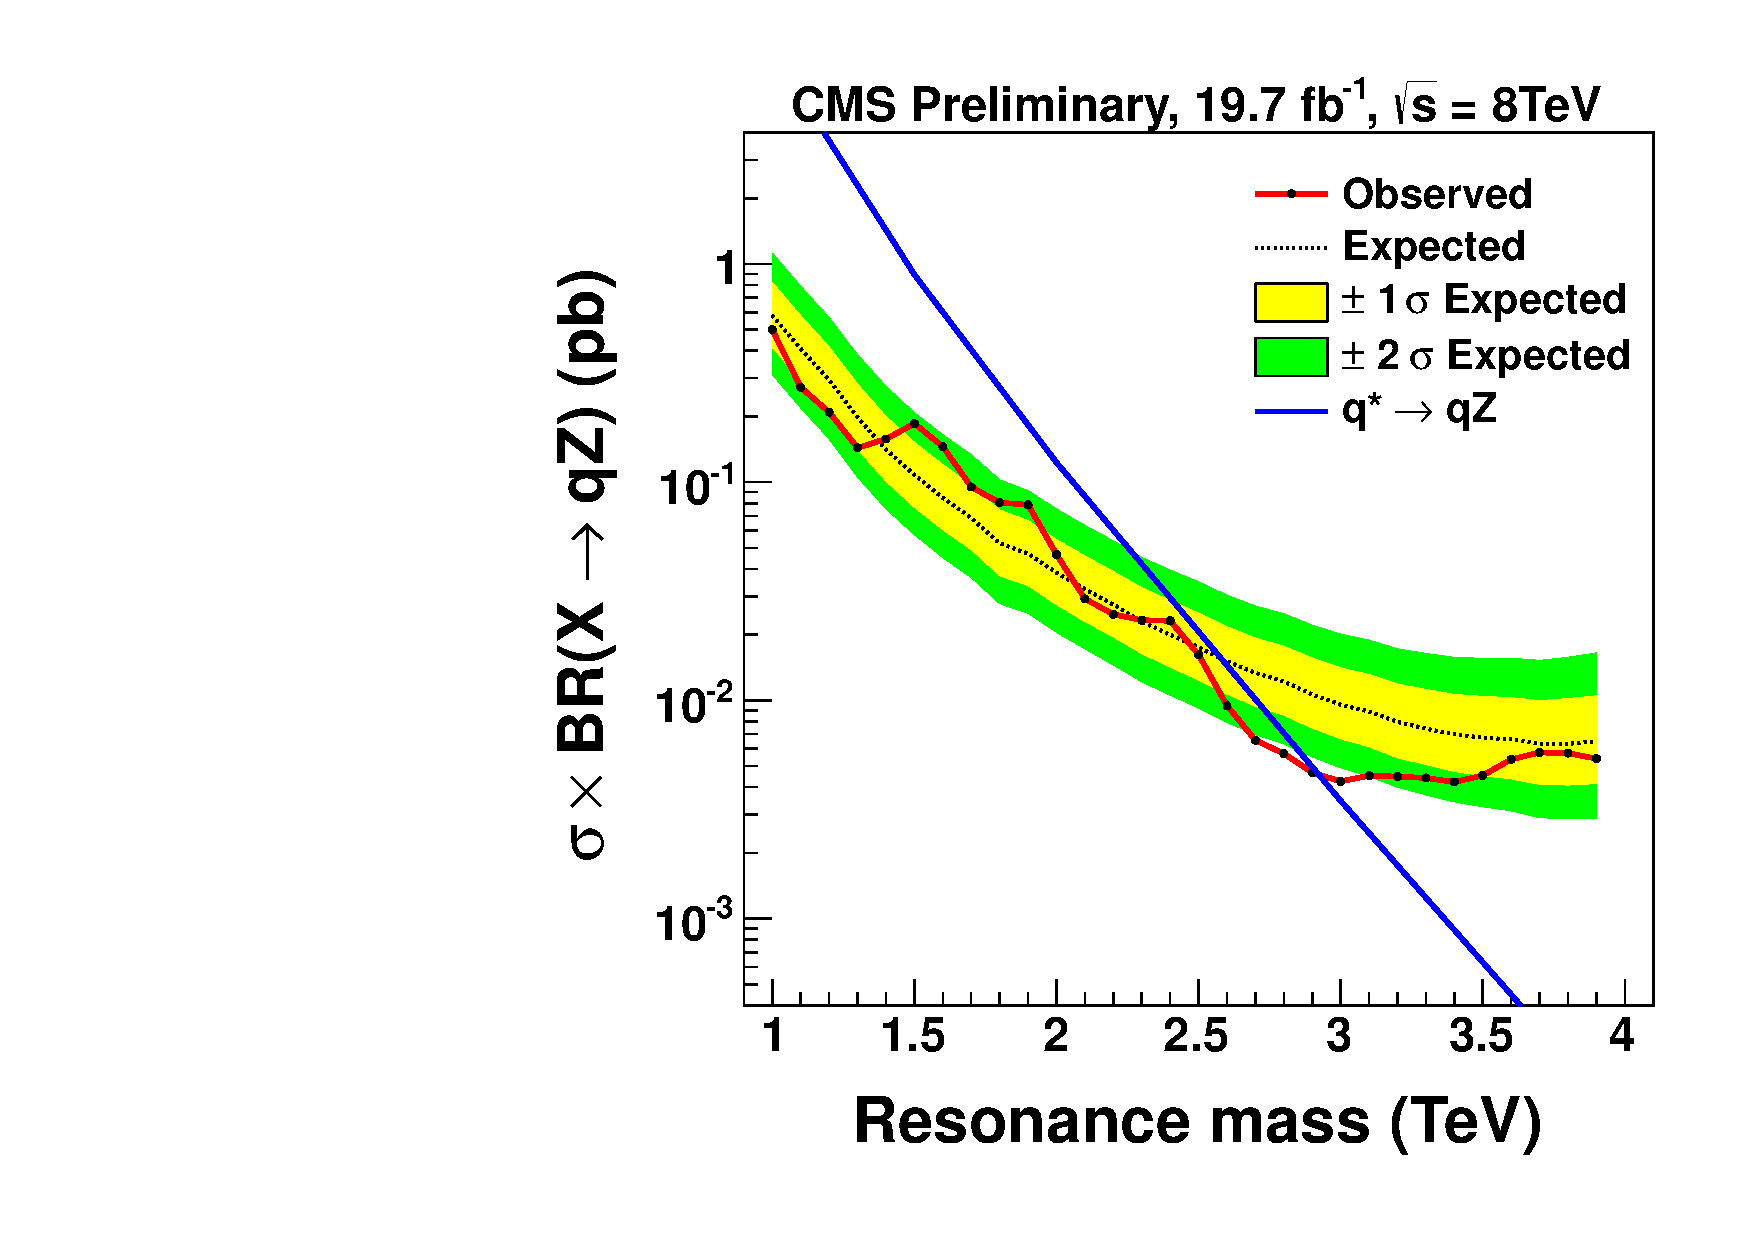
\includegraphics[width=0.35\textwidth]{figs/limits/brazilianFlag_qZ_high_purity.pdf}\\
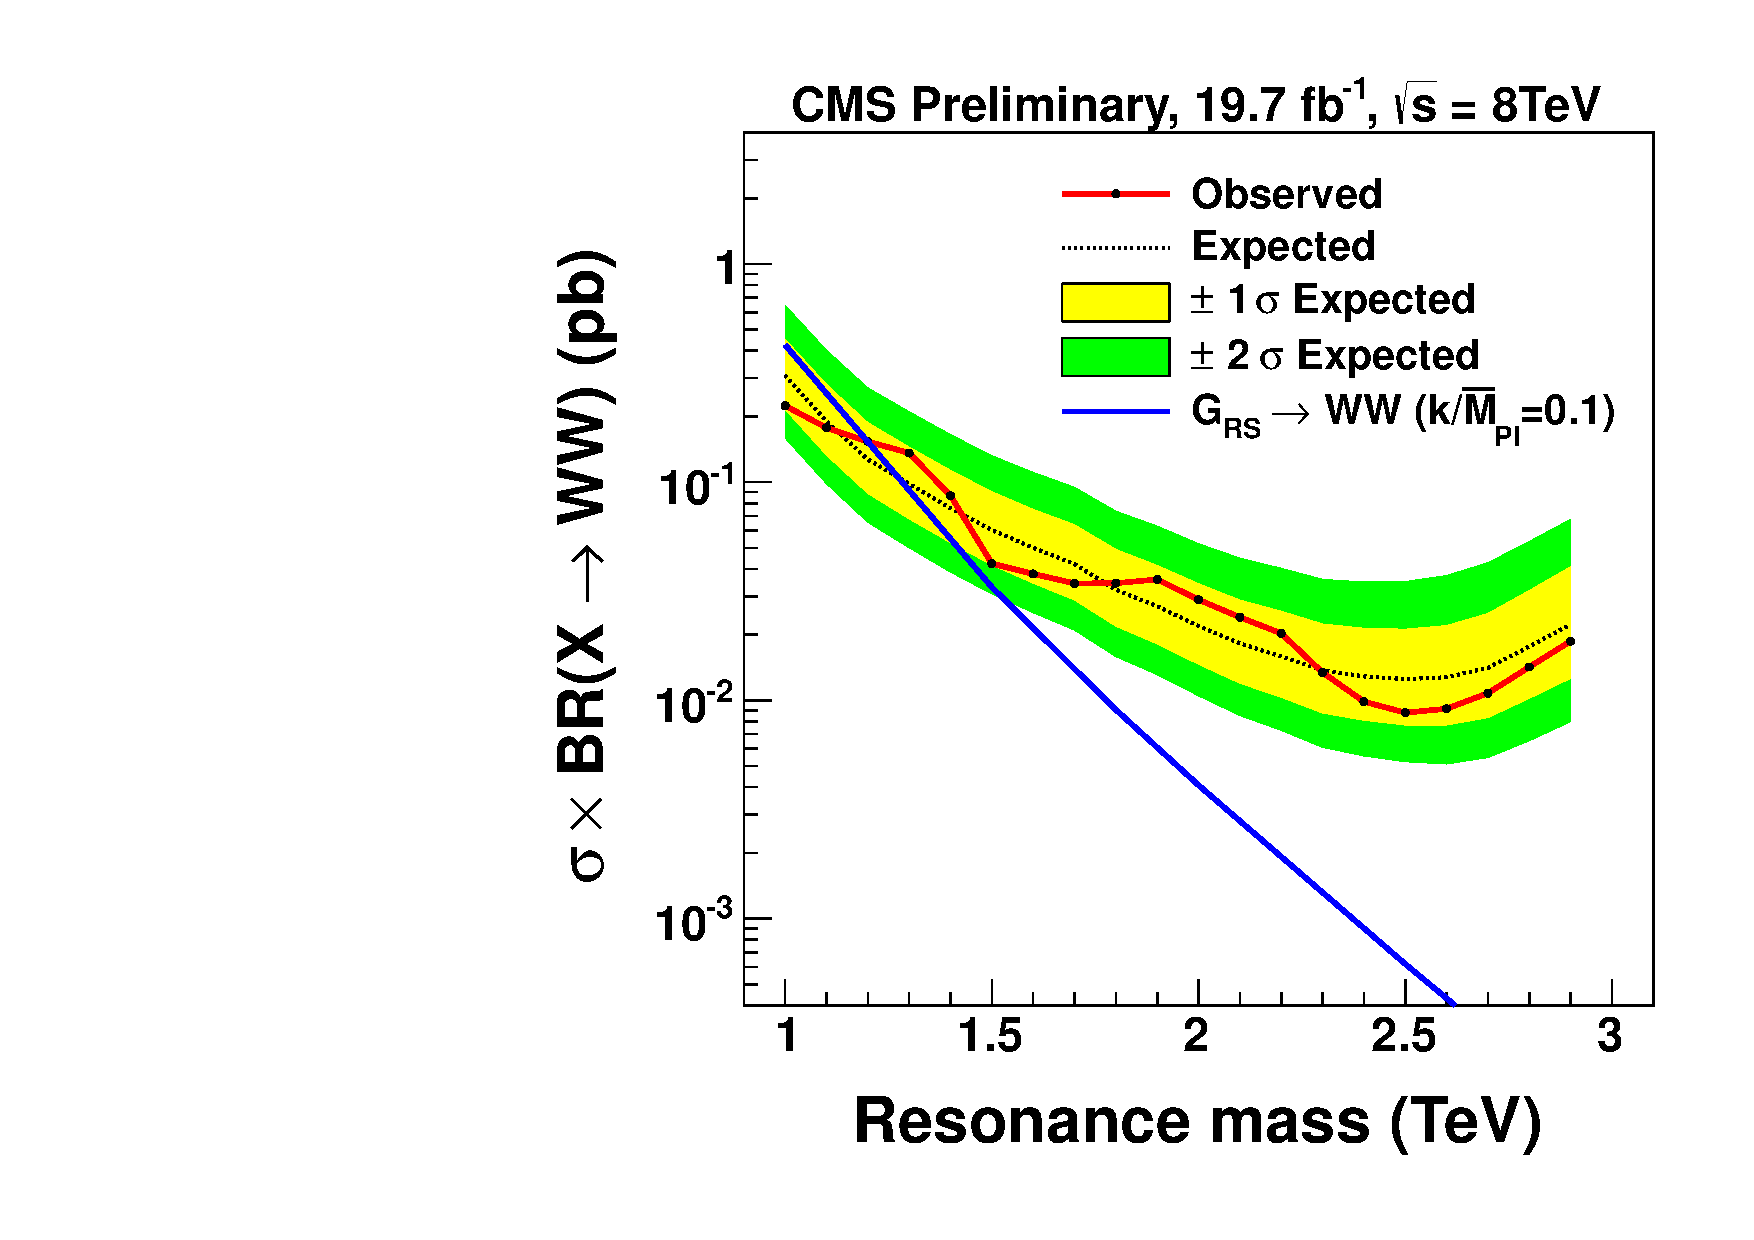
\includegraphics[width=0.35\textwidth]{figs/limits/brazilianFlag_RS1WW_high_purity.pdf}
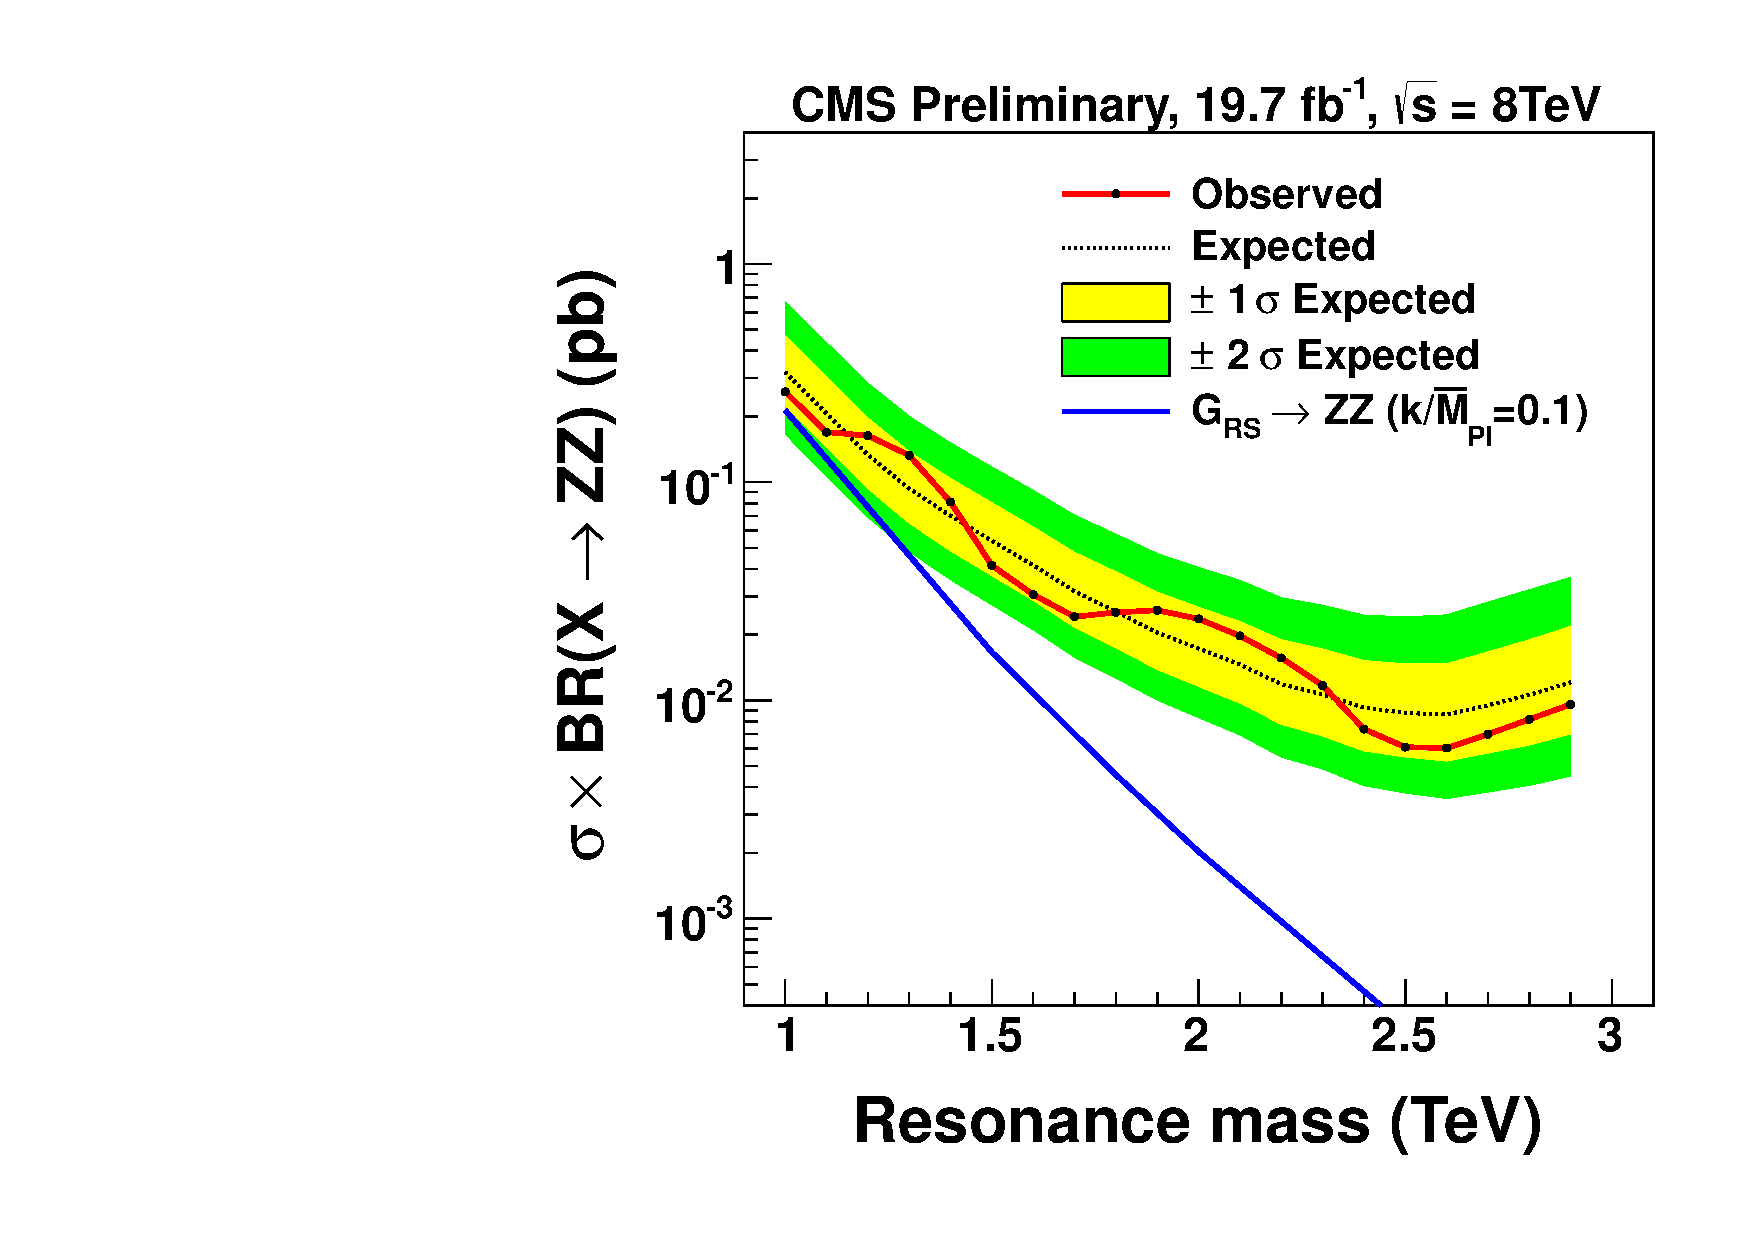
\includegraphics[width=0.35\textwidth]{figs/limits/brazilianFlag_RS1ZZ_high_purity.pdf}\\
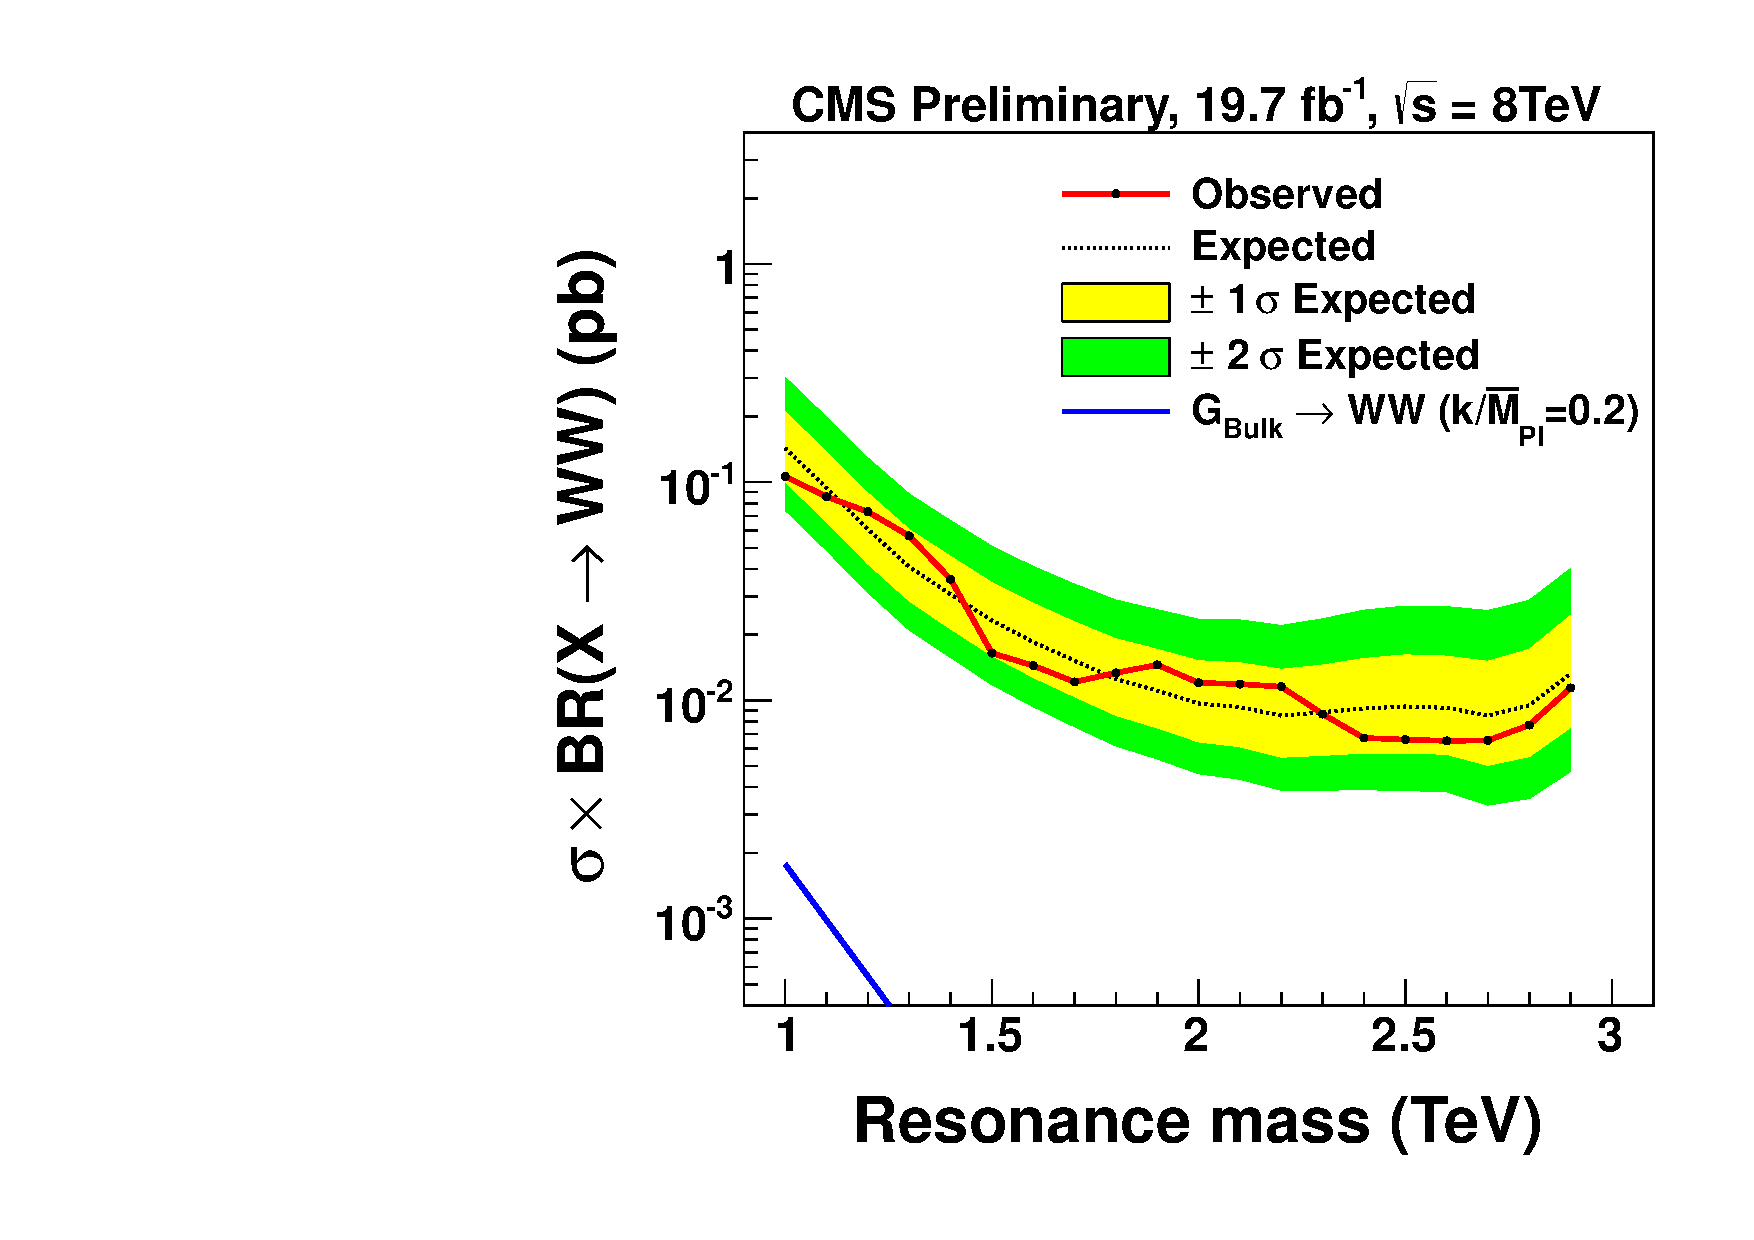
\includegraphics[width=0.35\textwidth]{figs/limits/brazilianFlag_BulkWW_high_purity.pdf}
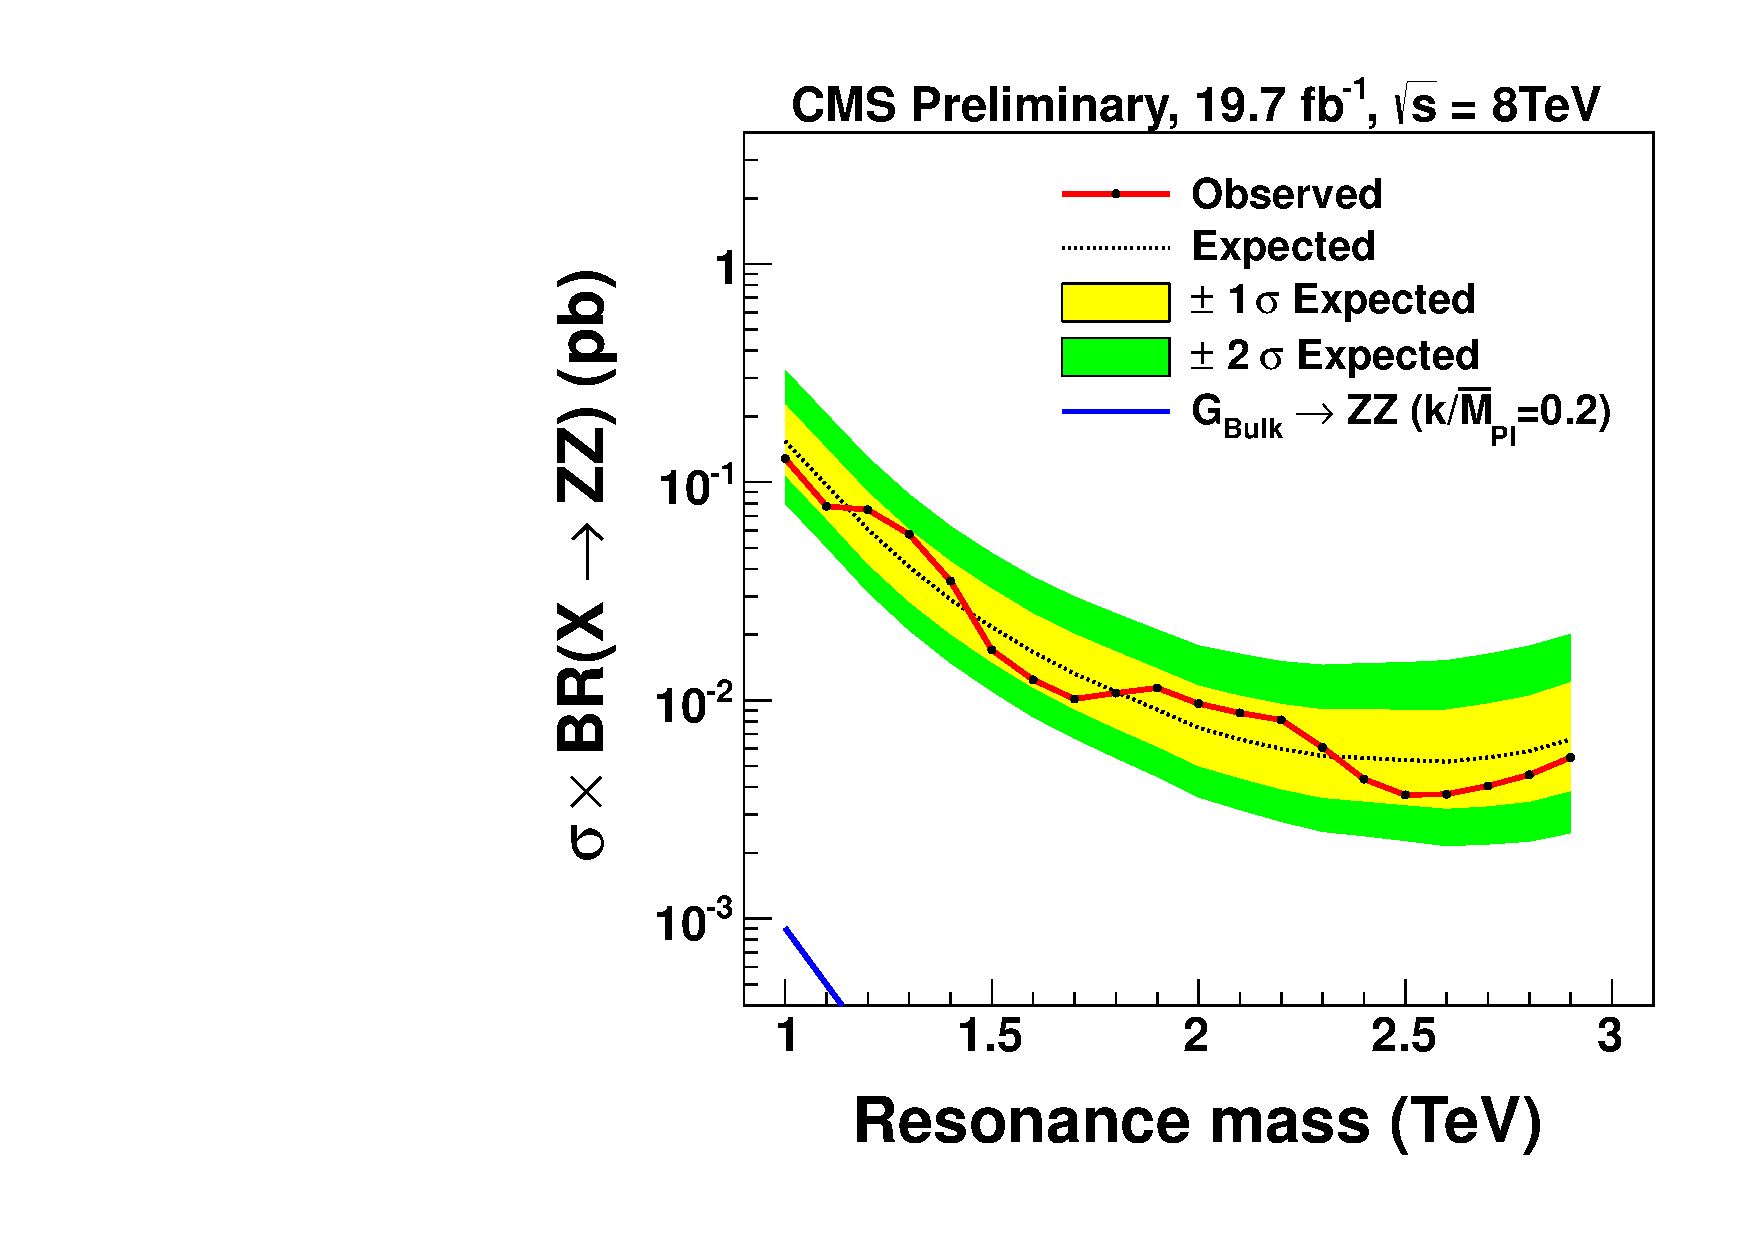
\includegraphics[width=0.35\textwidth]{figs/limits/brazilianFlag_BulkZZ_high_purity.pdf}\\
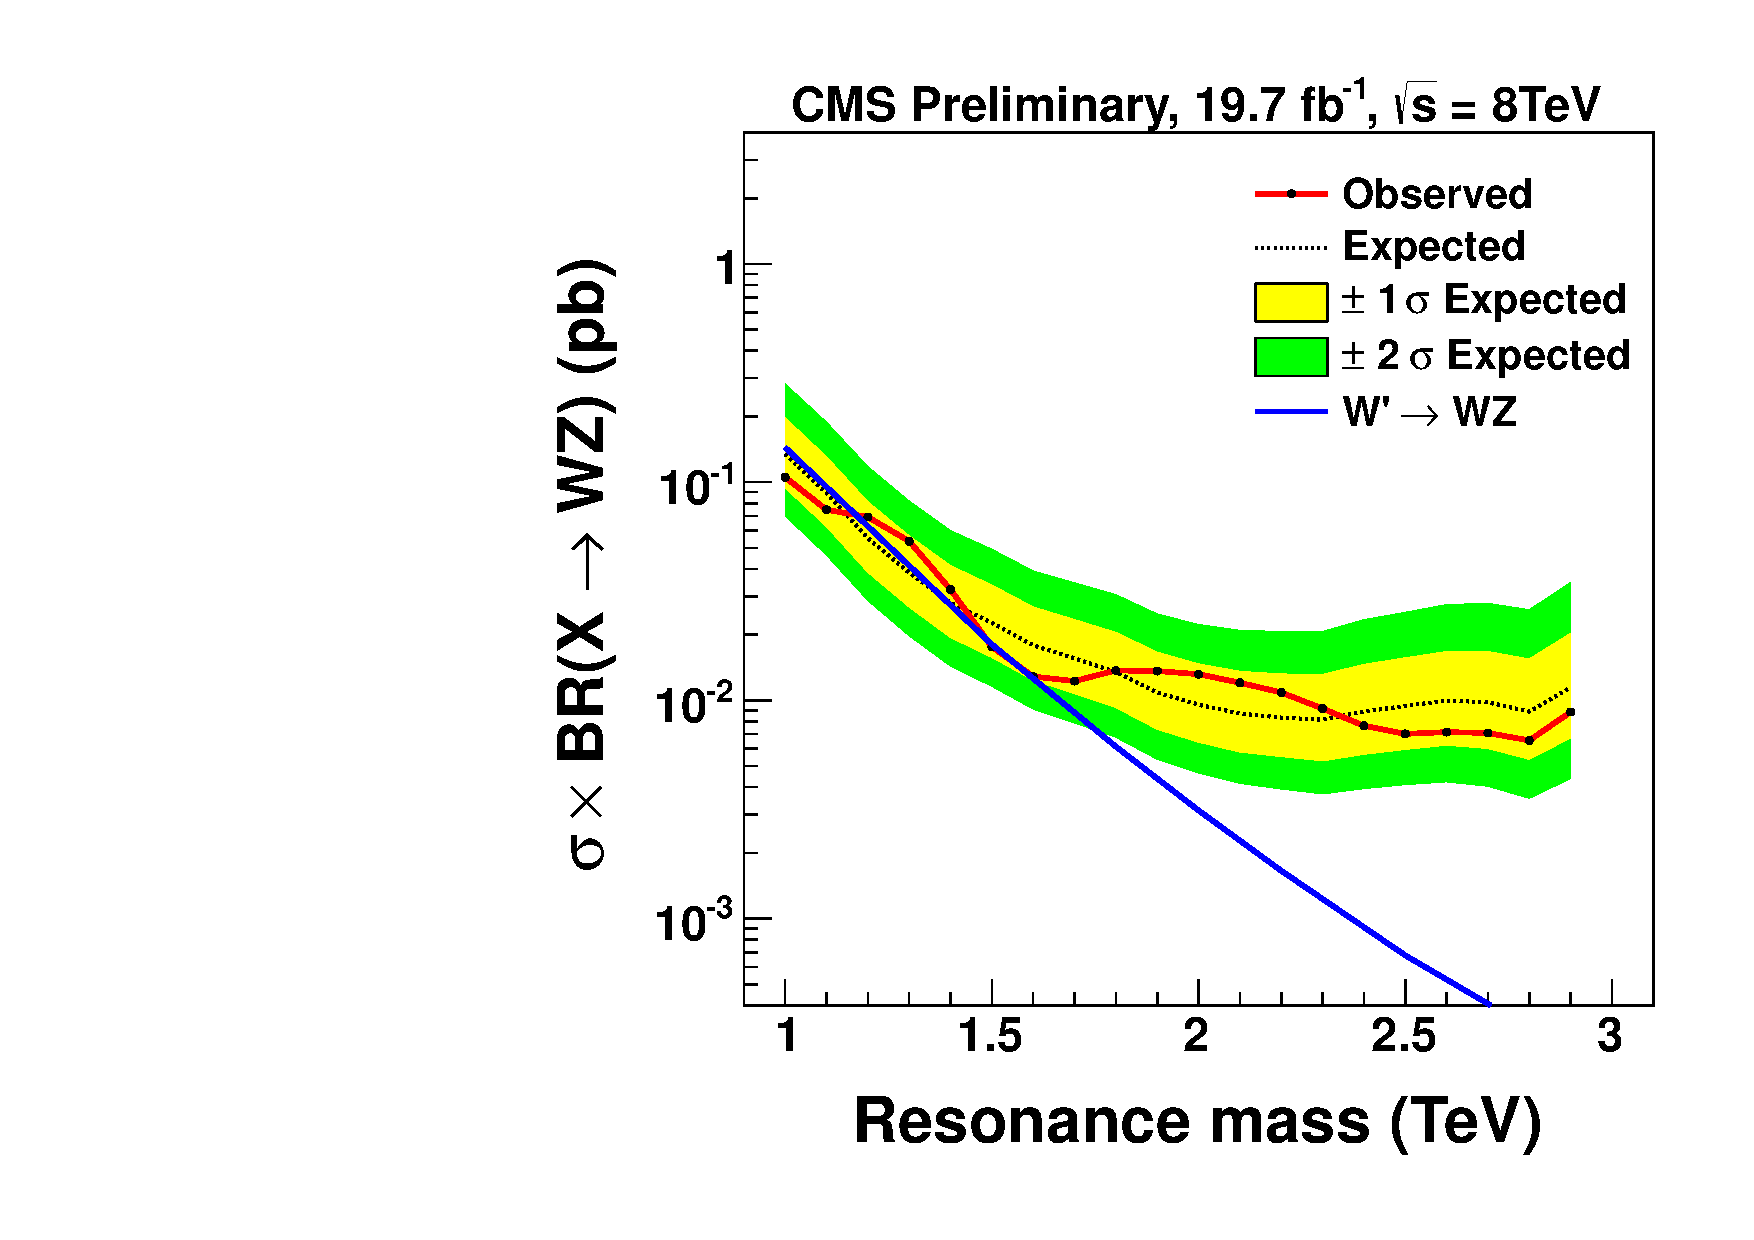
\includegraphics[width=0.35\textwidth]{figs/limits/brazilianFlag_WZ_high_purity.pdf}
\end{center}
\caption{Expected and observed limits for qW (top-left), qZ (top-right), \GRS WW (center-left), \GRS ZZ (center-right), \GBulk WW (center-left), \GBulk ZZ (center-right) and WZ (bottom) resonances in the high-purity category.
  The predicted cross sections as a function of resonance mass for the considered benchmark models are overlaid.}
\label{fig:Vtagresults1}
\end{figure*}

\begin{figure*}[h!tpb]
\begin{center}
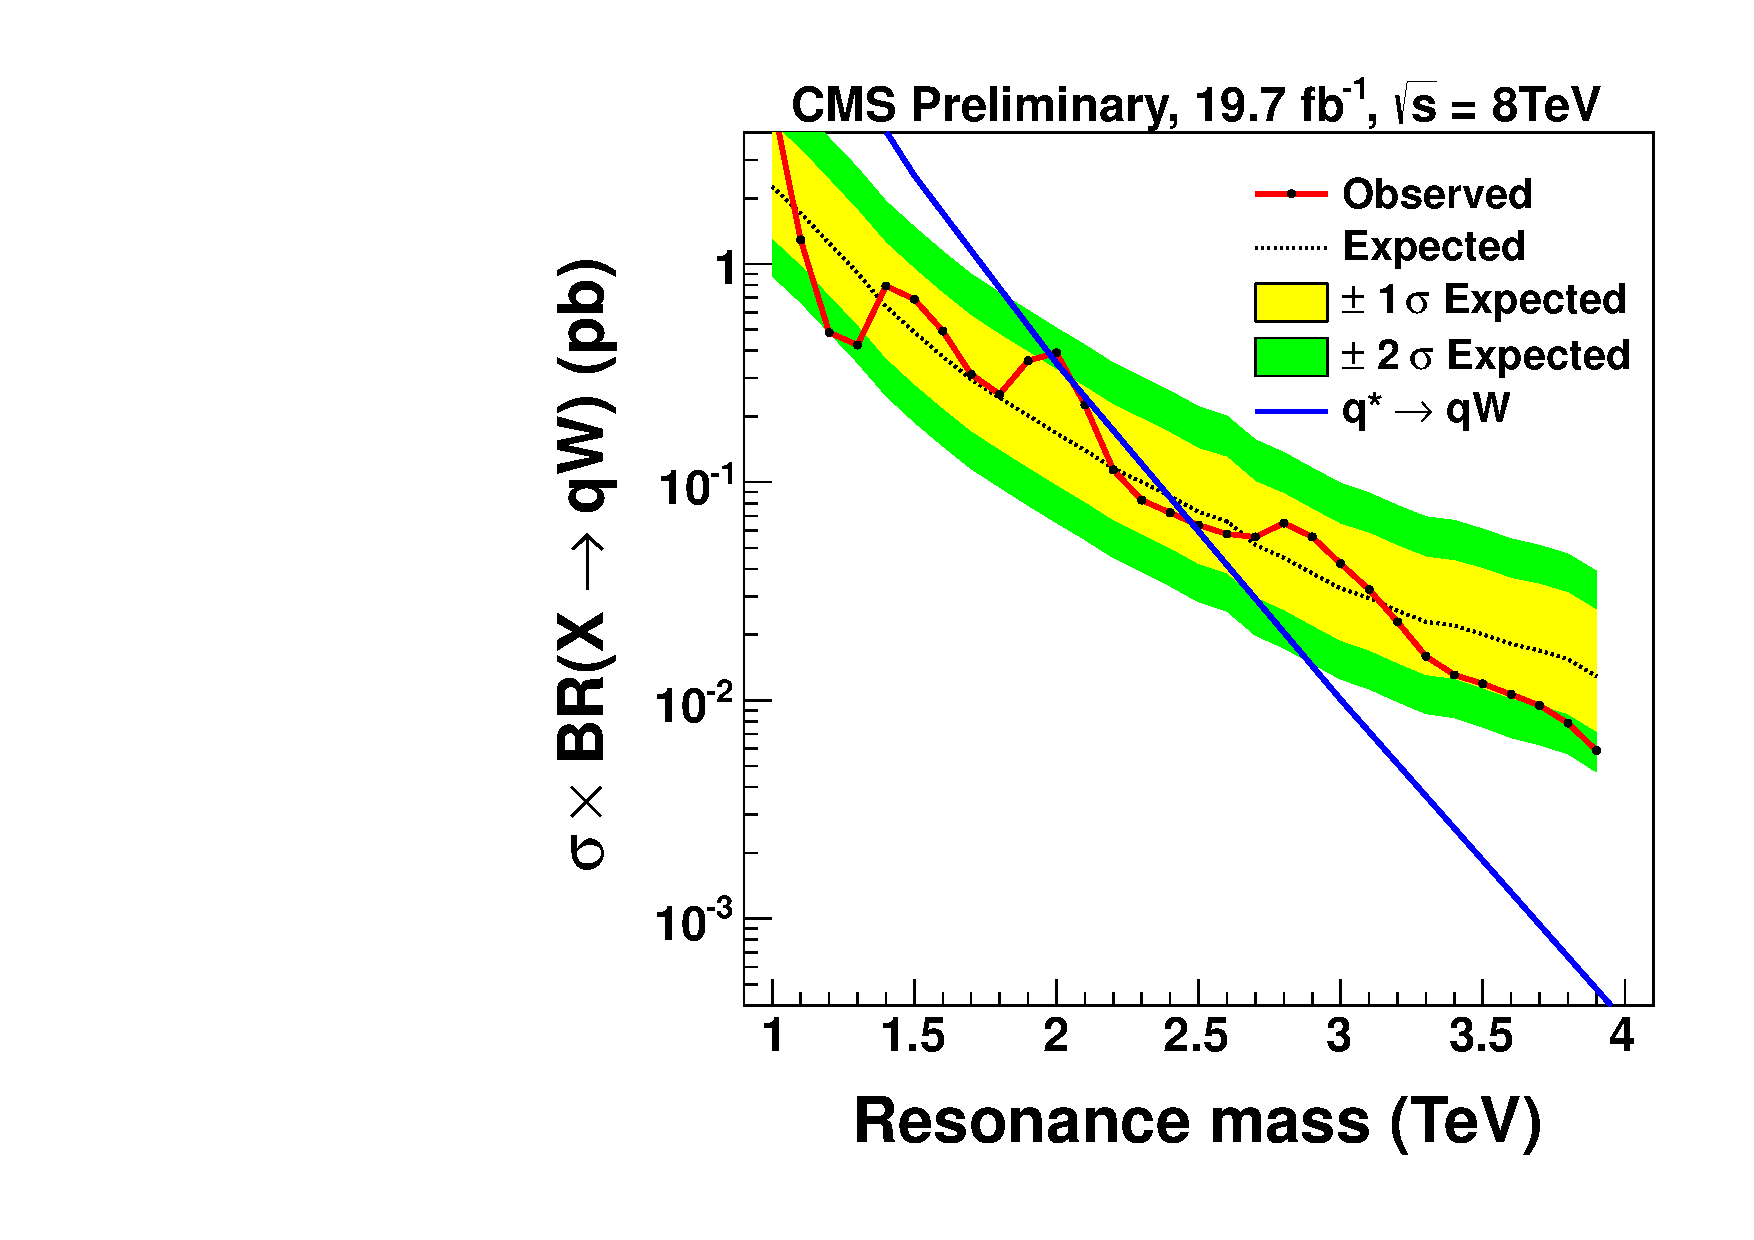
\includegraphics[width=0.35\textwidth]{figs/limits/brazilianFlag_qW_low_purity.pdf}
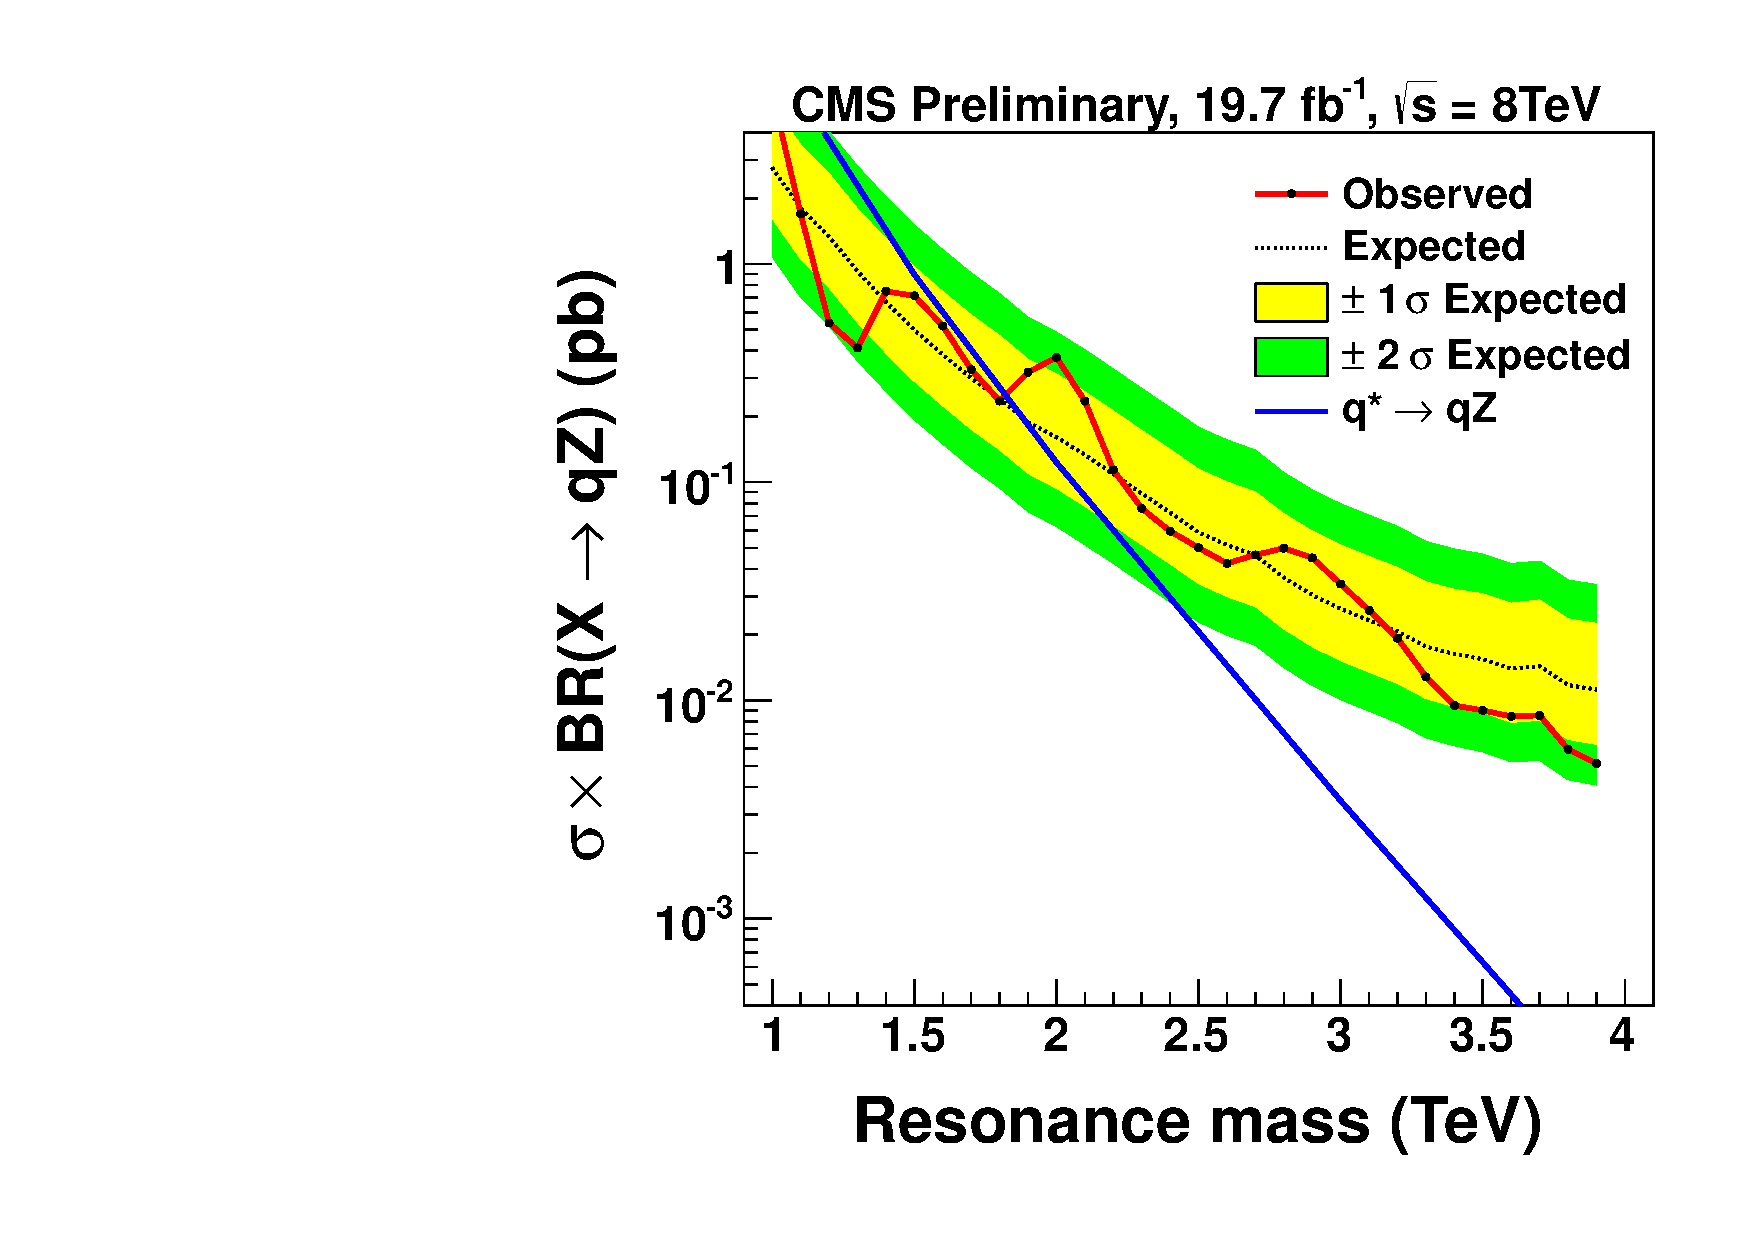
\includegraphics[width=0.35\textwidth]{figs/limits/brazilianFlag_qZ_low_purity.pdf}\\
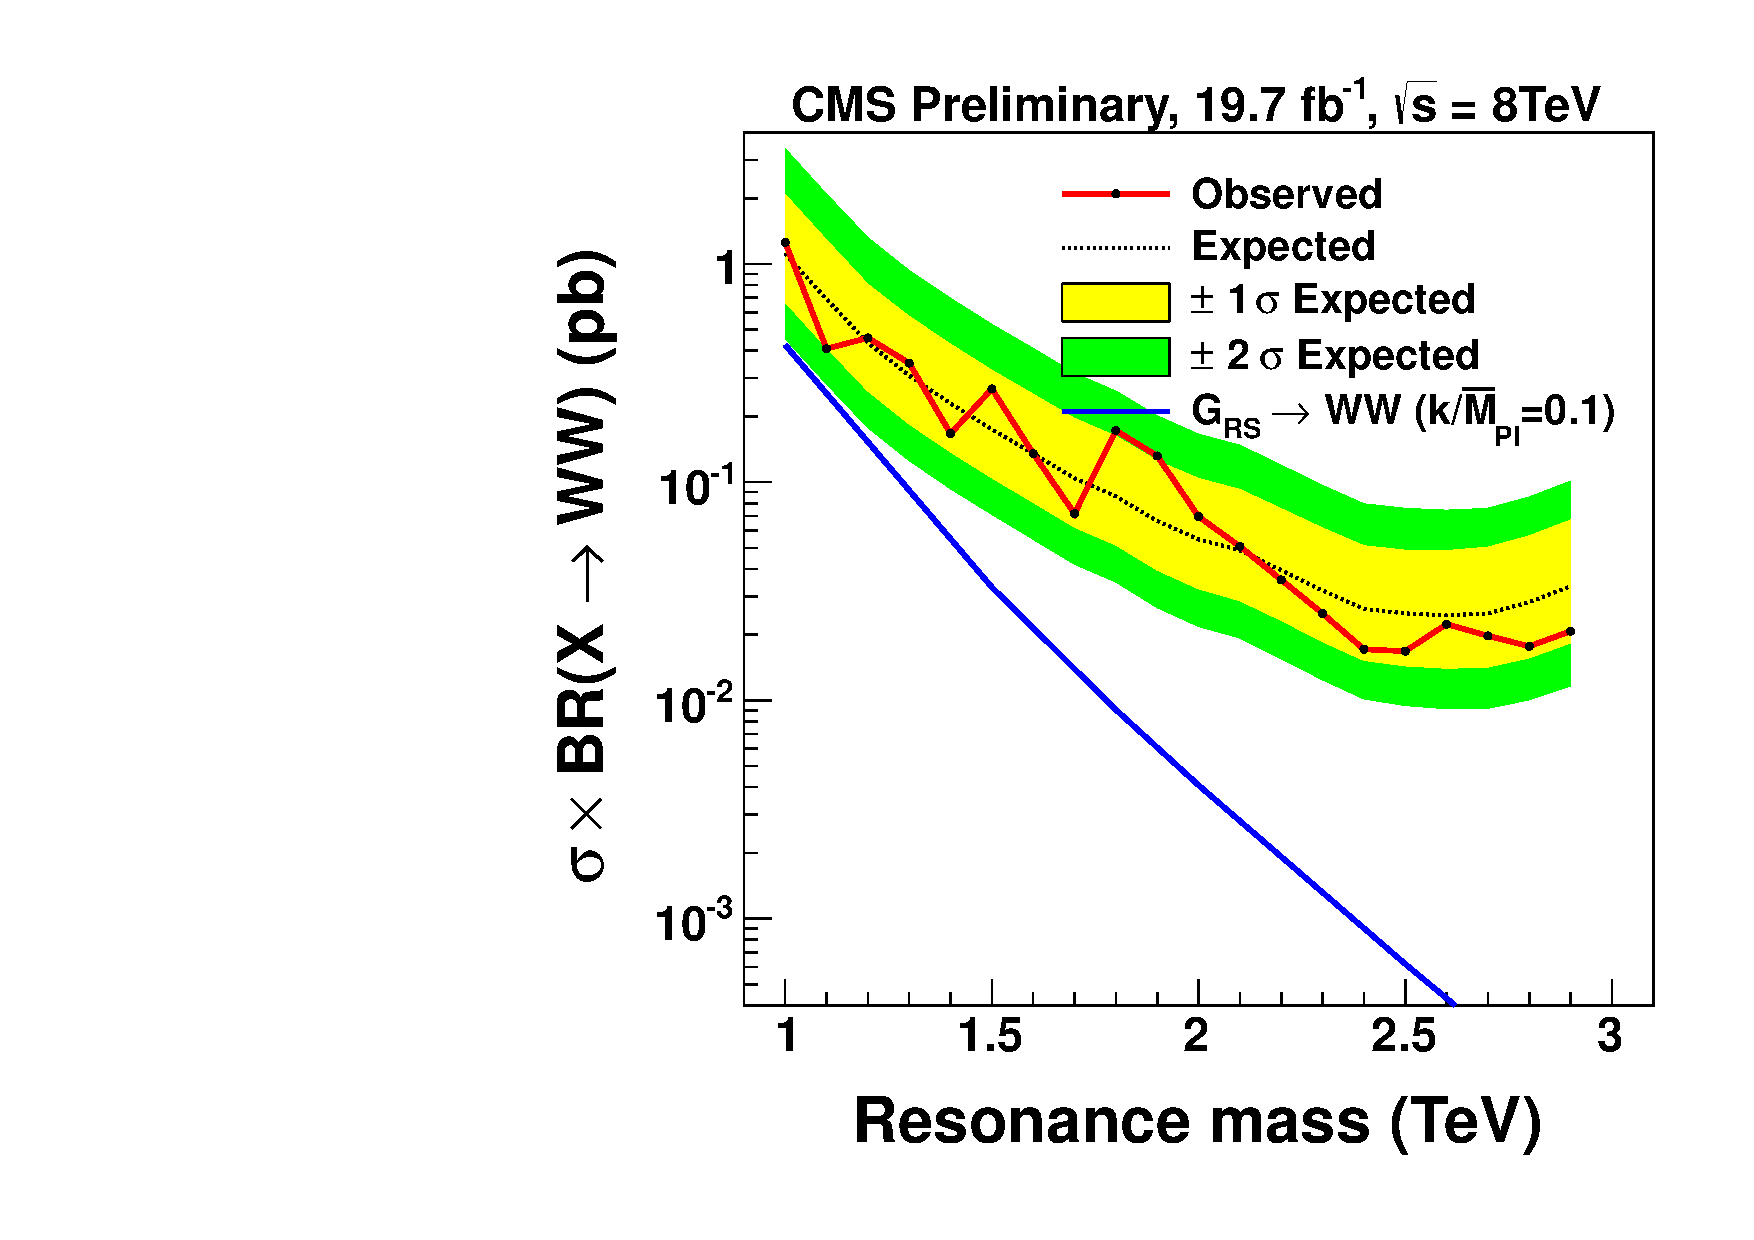
\includegraphics[width=0.35\textwidth]{figs/limits/brazilianFlag_RS1WW_low_purity.pdf}
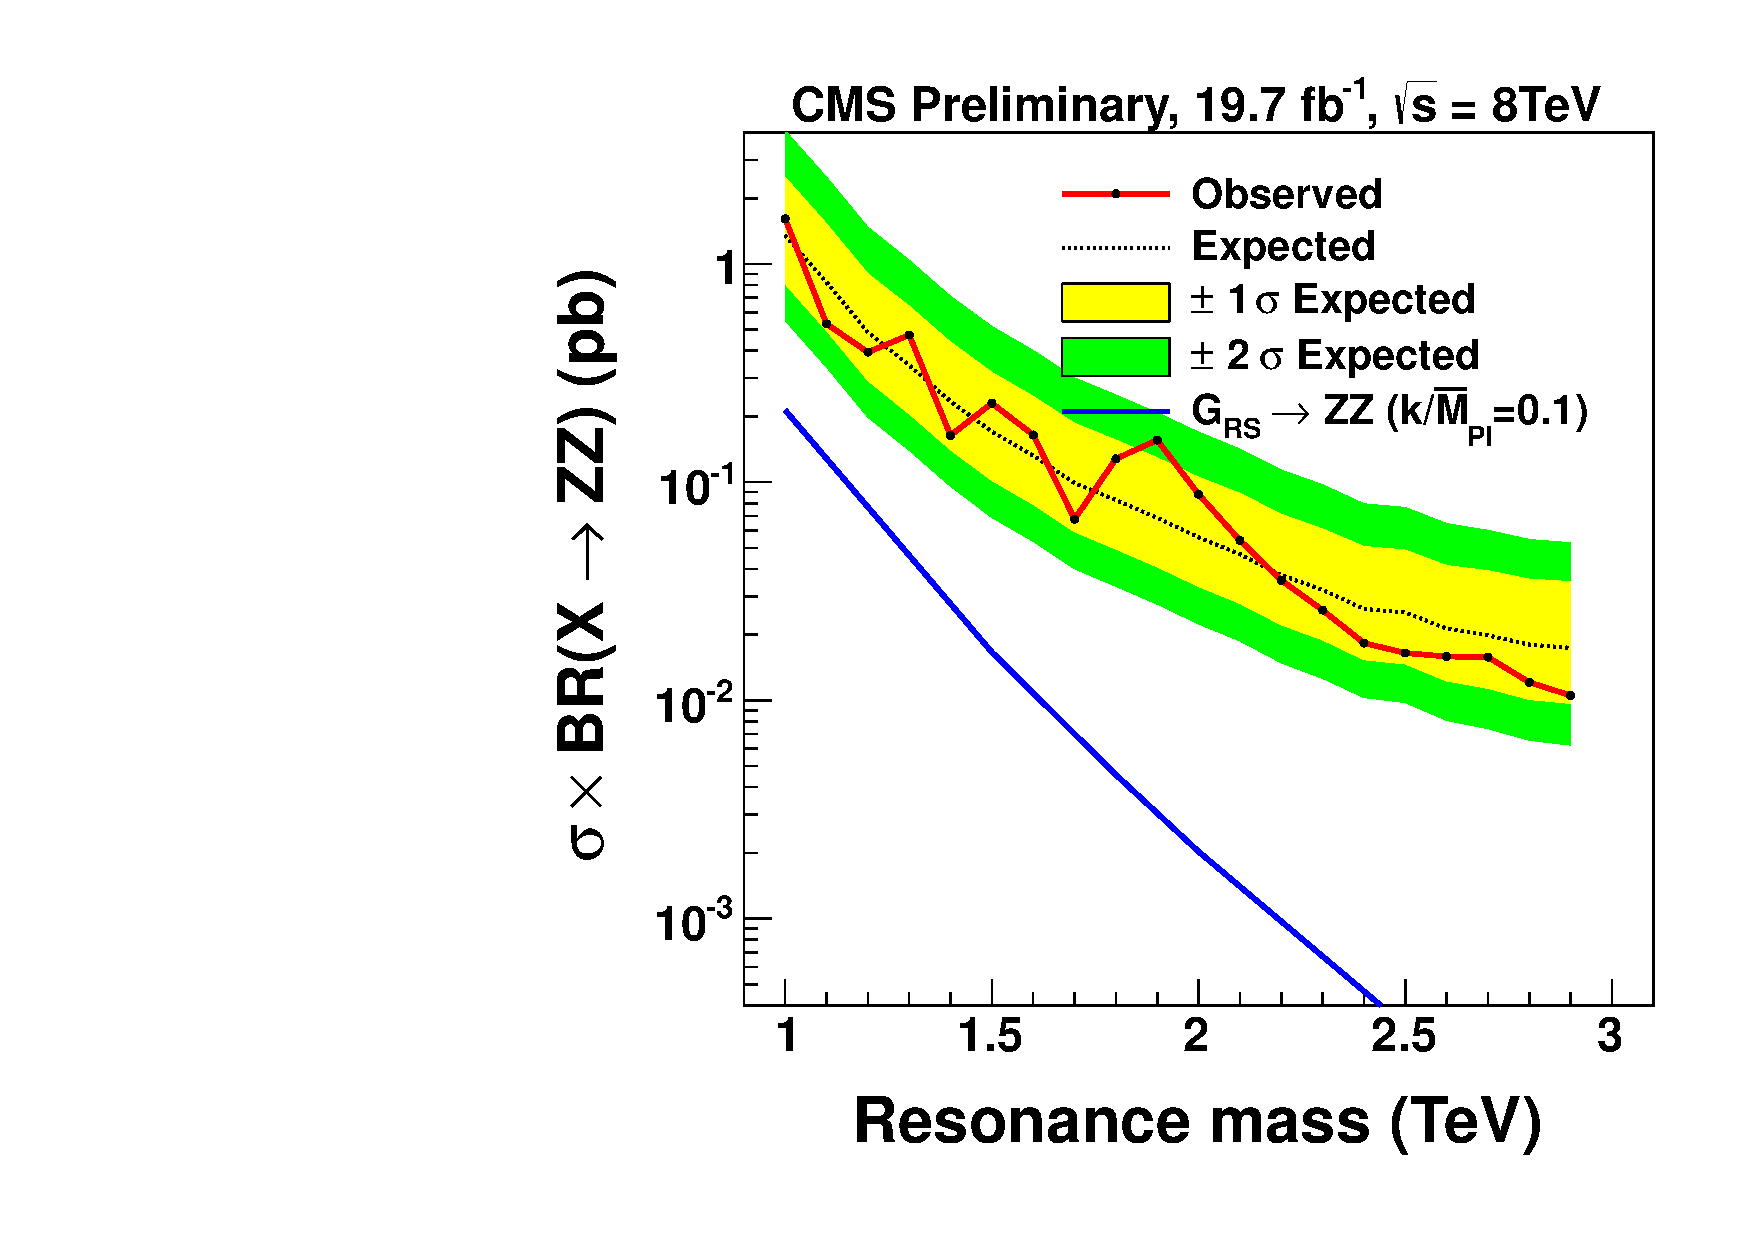
\includegraphics[width=0.35\textwidth]{figs/limits/brazilianFlag_RS1ZZ_low_purity.pdf}\\
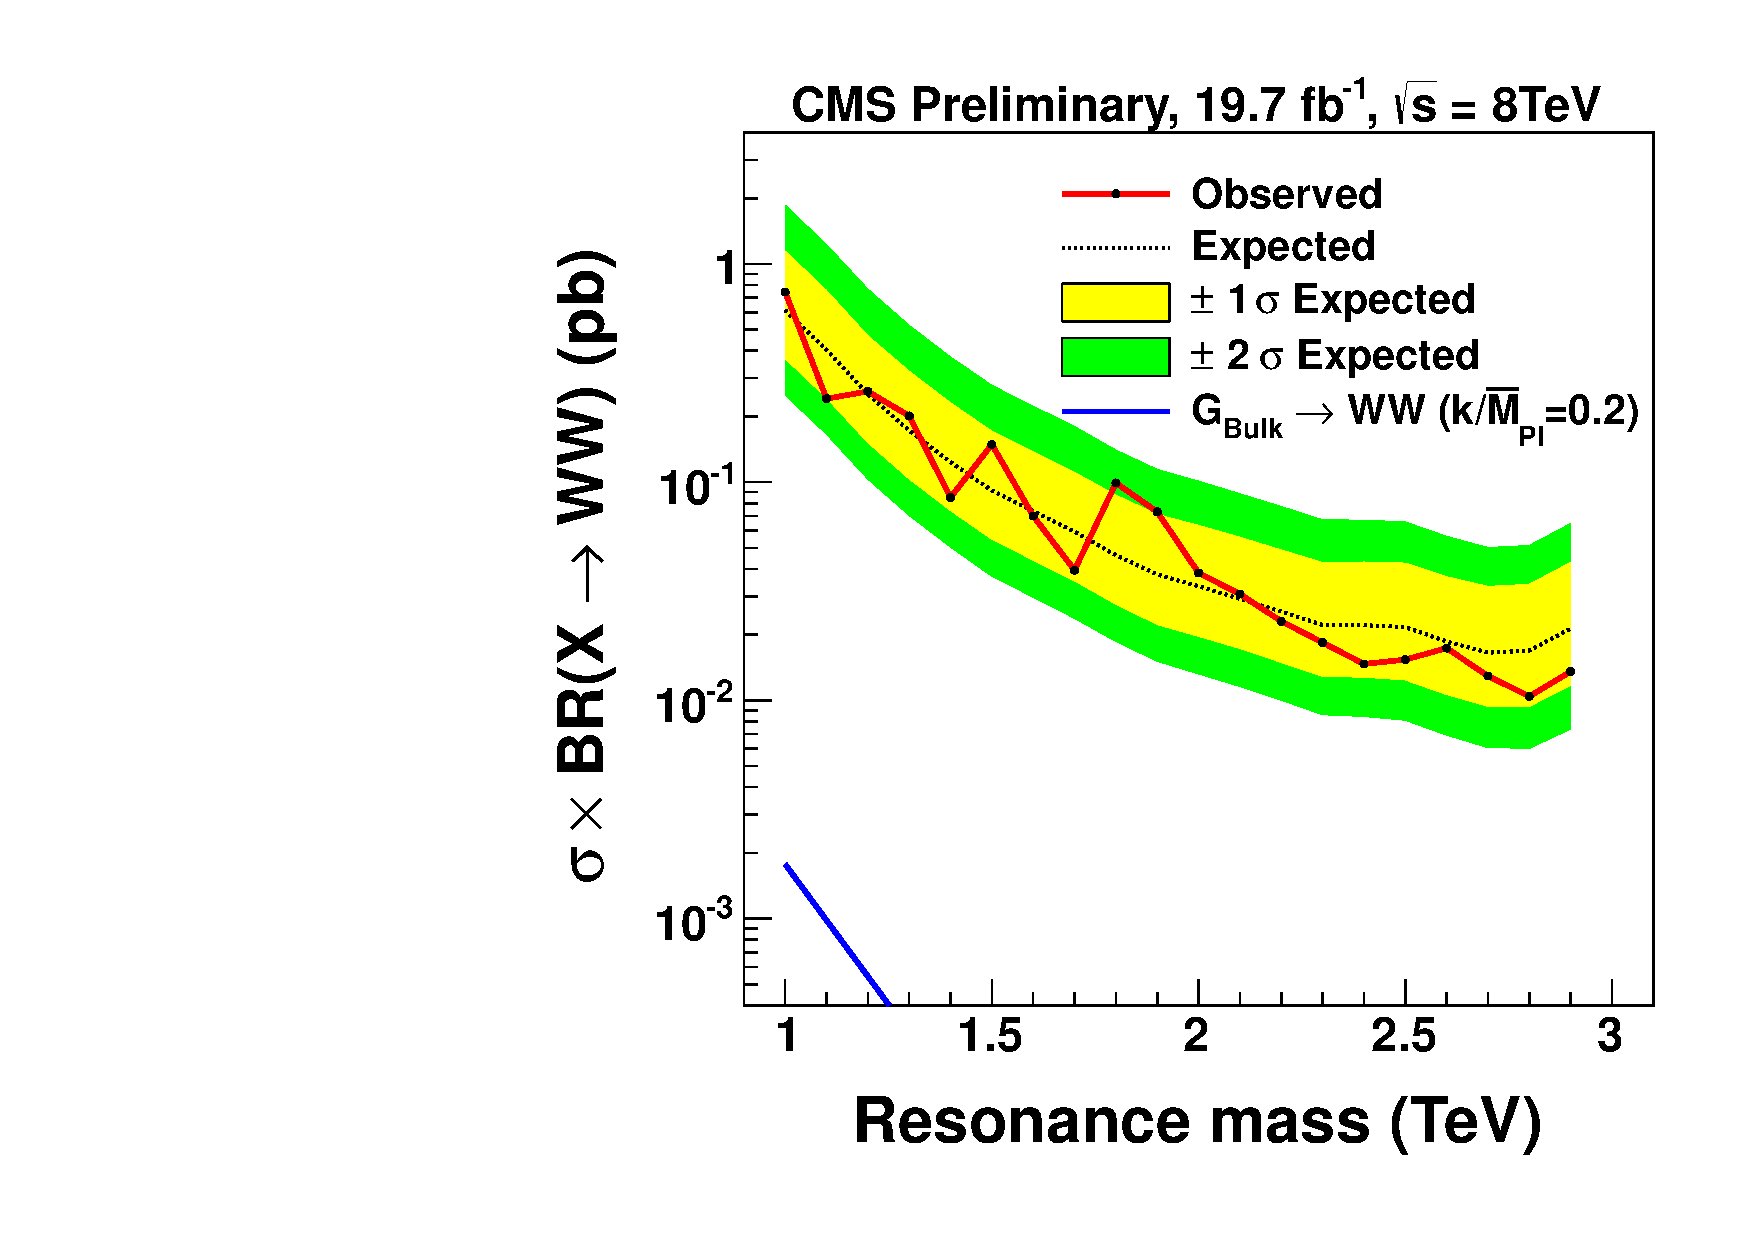
\includegraphics[width=0.35\textwidth]{figs/limits/brazilianFlag_BulkWW_low_purity.pdf}
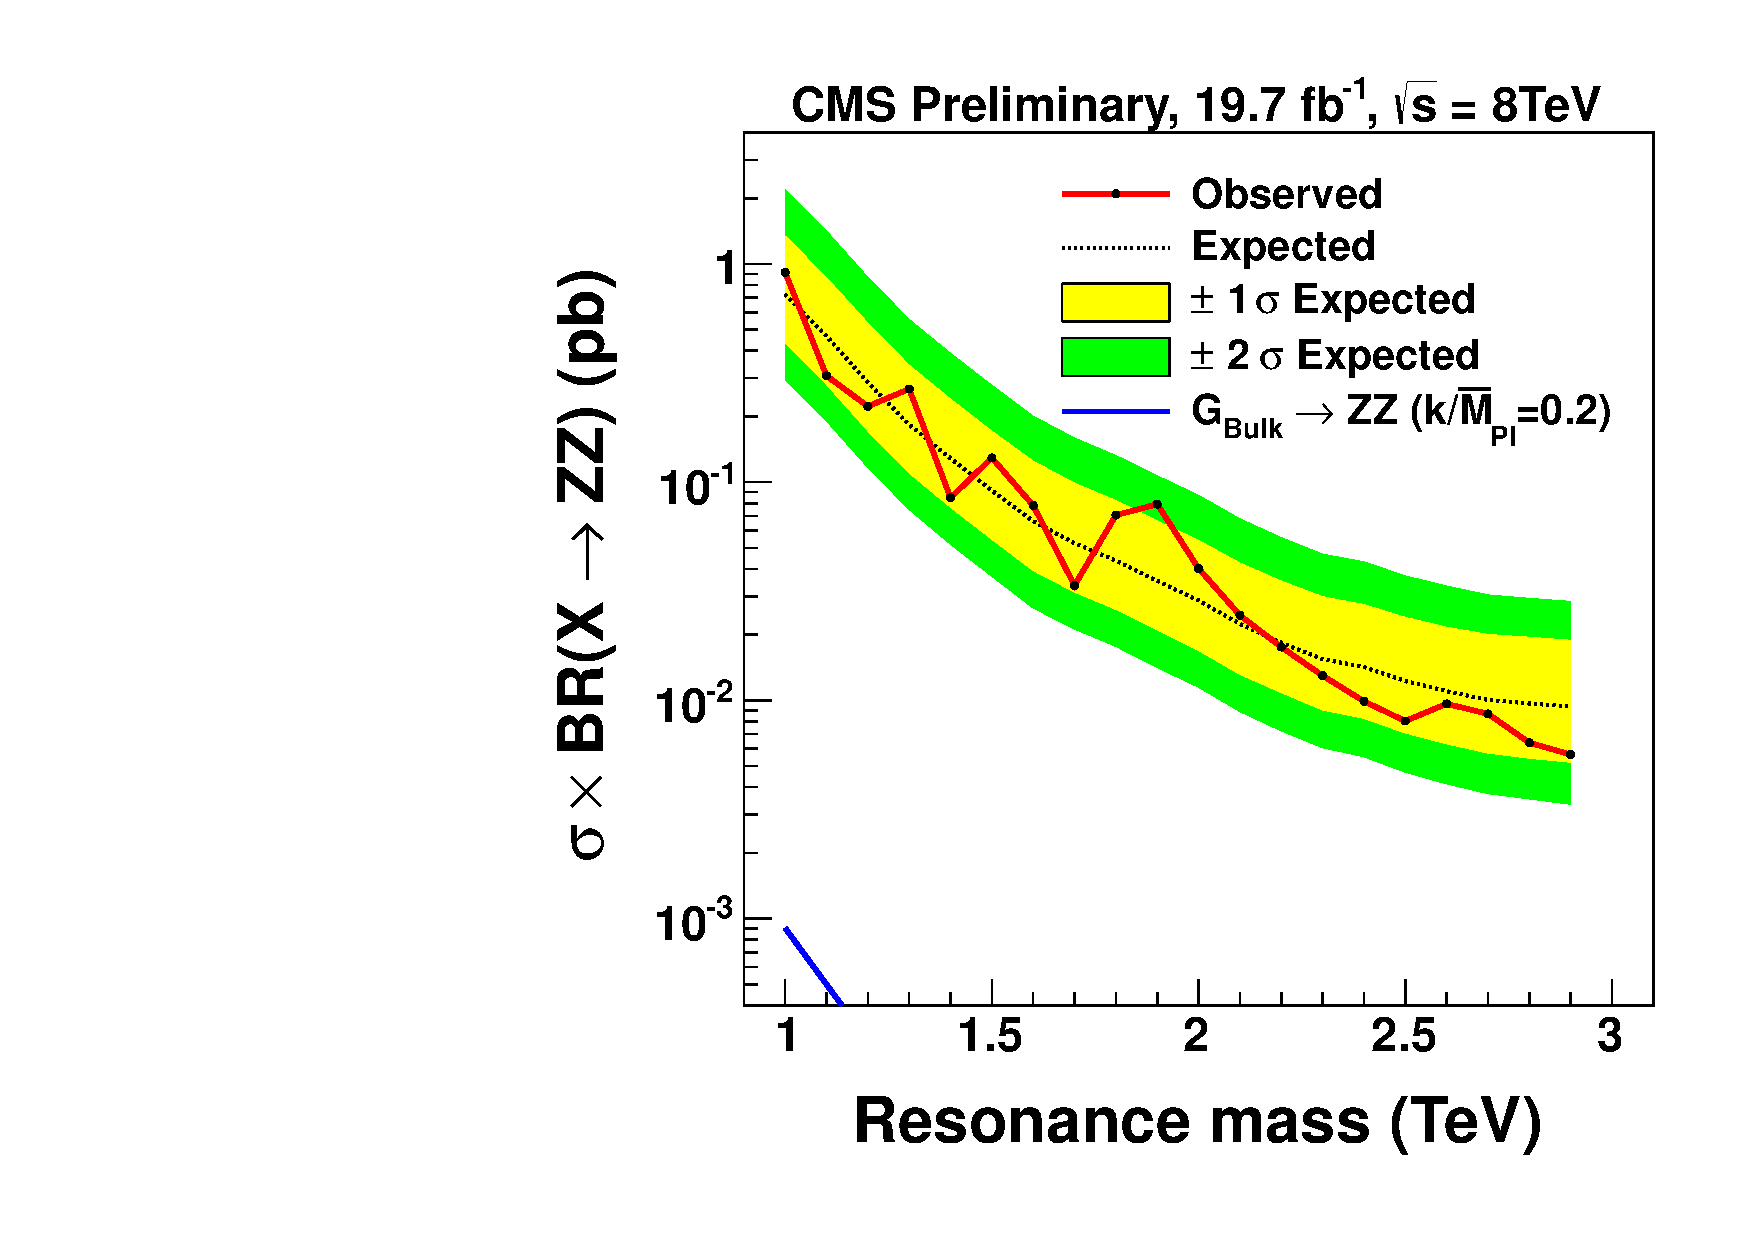
\includegraphics[width=0.35\textwidth]{figs/limits/brazilianFlag_BulkZZ_low_purity.pdf}\\
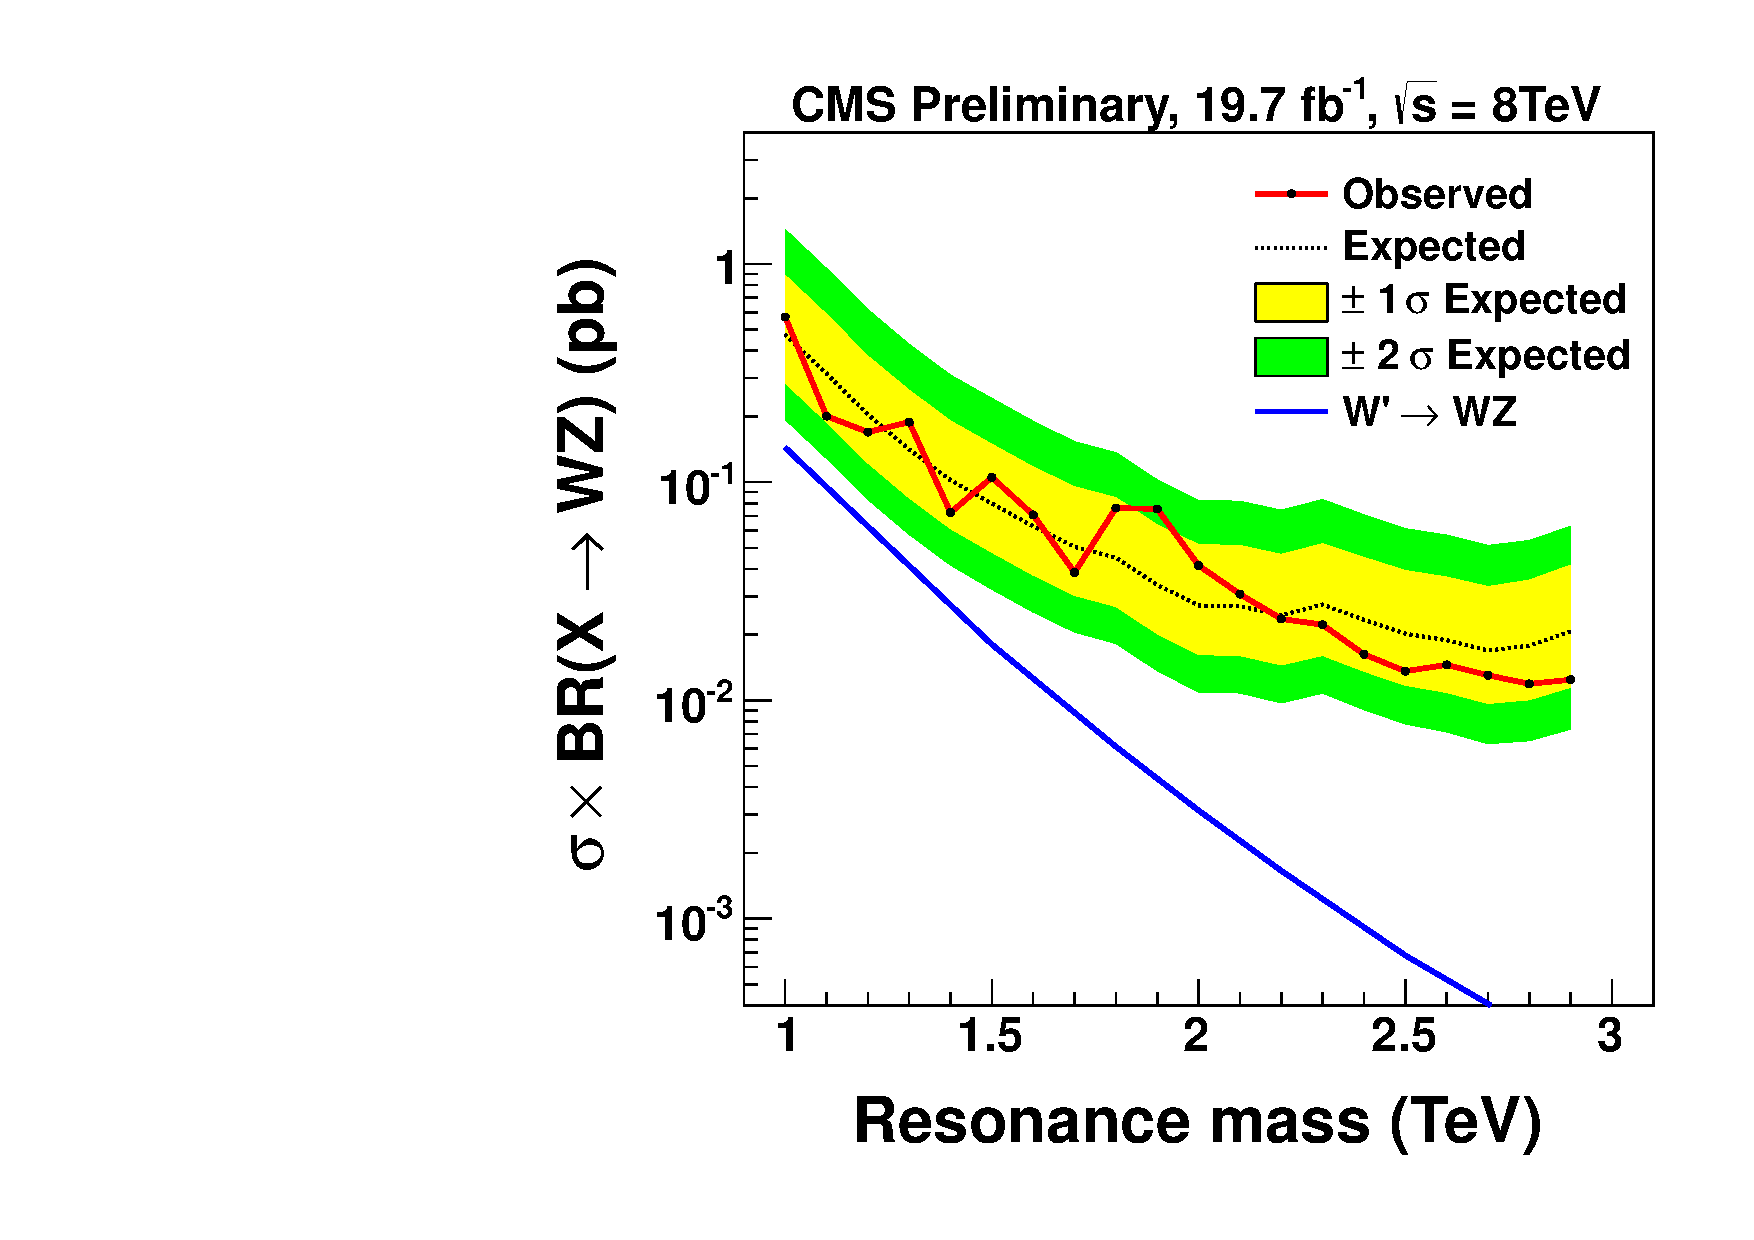
\includegraphics[width=0.35\textwidth]{figs/limits/brazilianFlag_WZ_low_purity.pdf}
\end{center}
\caption{Expected and observed limits for qW (top-left), qZ (top-right), \GRS WW (center-left), \GRS ZZ (center-right), \GBulk WW (center-left), \GBulk ZZ (center-right) and WZ (bottom) resonances
 in the low-purity category.
  The predicted cross sections as a function of resonance mass for the considered benchmark models are overlaid.}
\label{fig:Vtagresults2}
\end{figure*}

\begin{figure*}[h!tpb]
\begin{center}
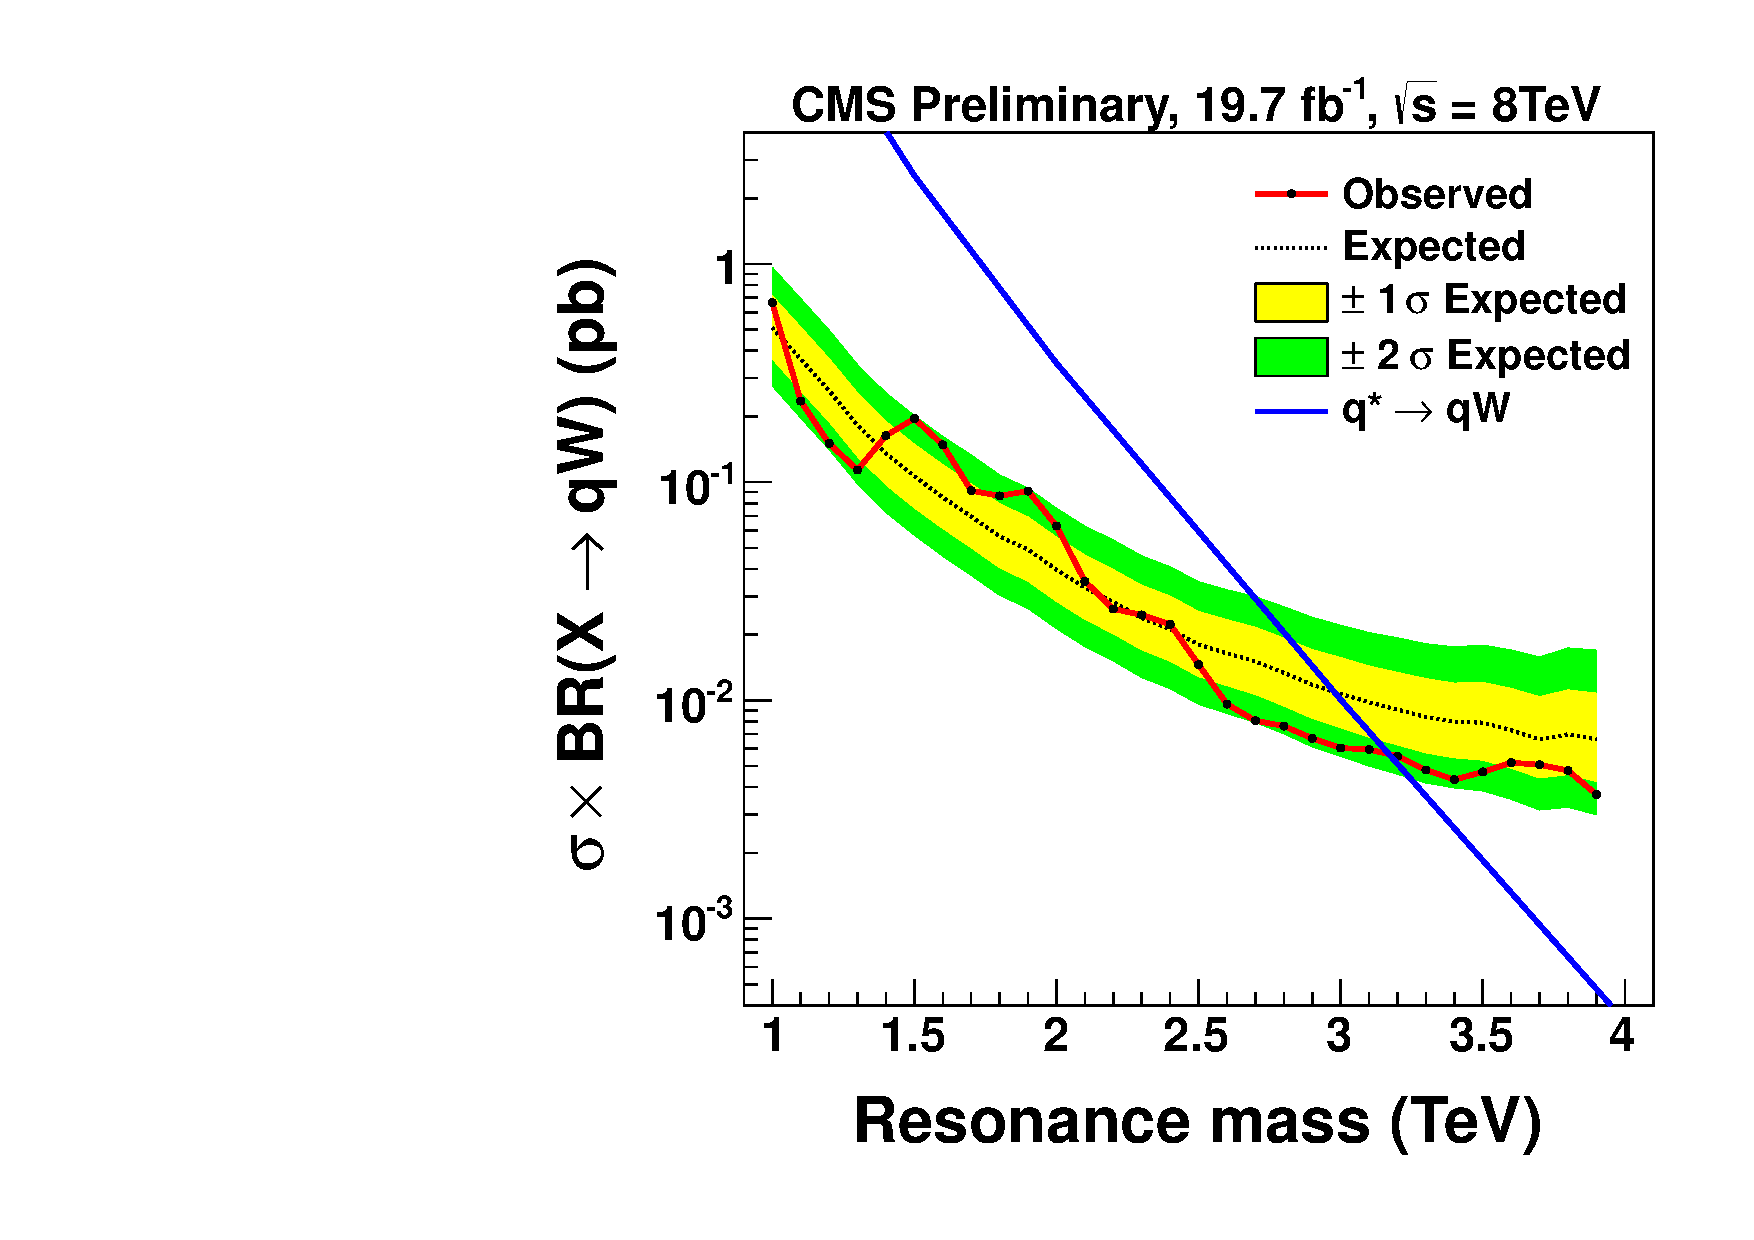
\includegraphics[width=0.35\textwidth]{figs/limits/brazilianFlag_qW_combined.pdf}
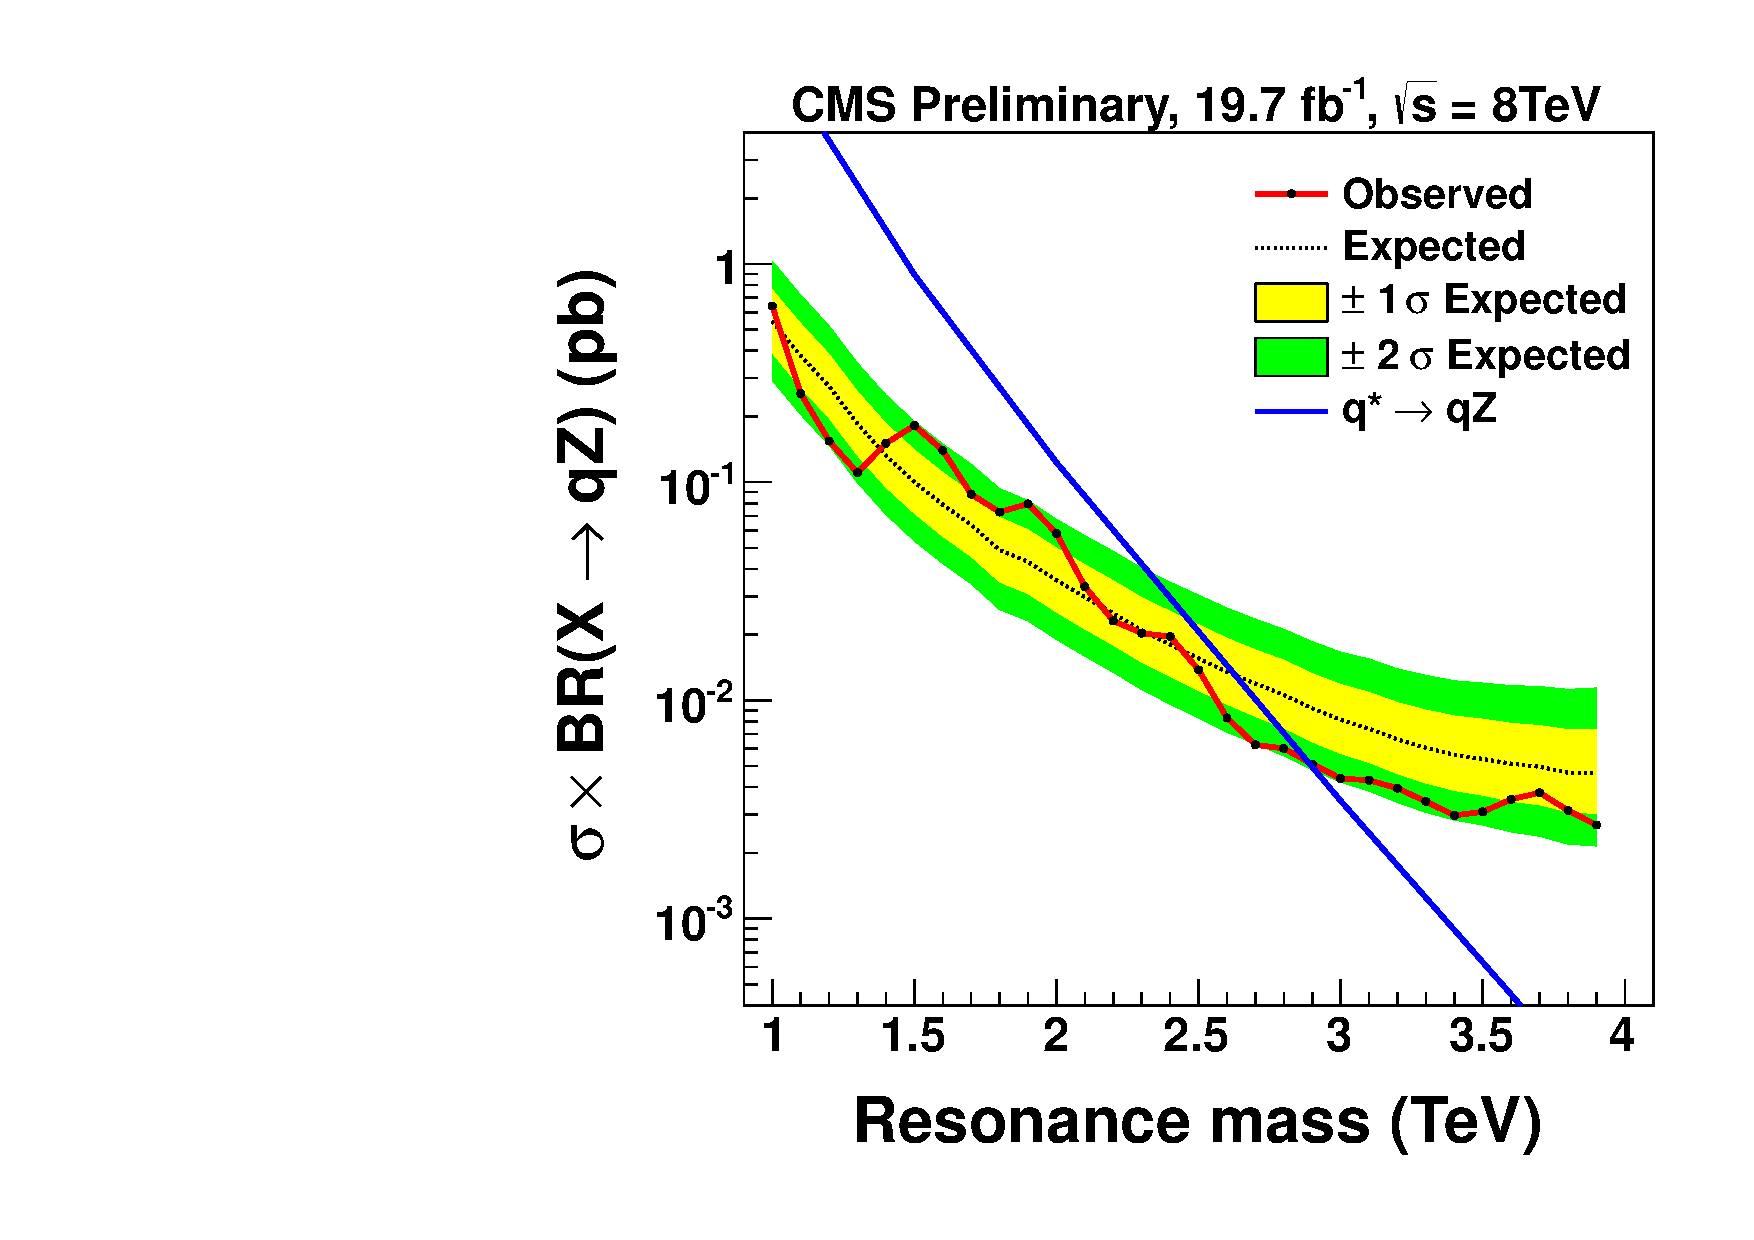
\includegraphics[width=0.35\textwidth]{figs/limits/brazilianFlag_qZ_combined.pdf}\\
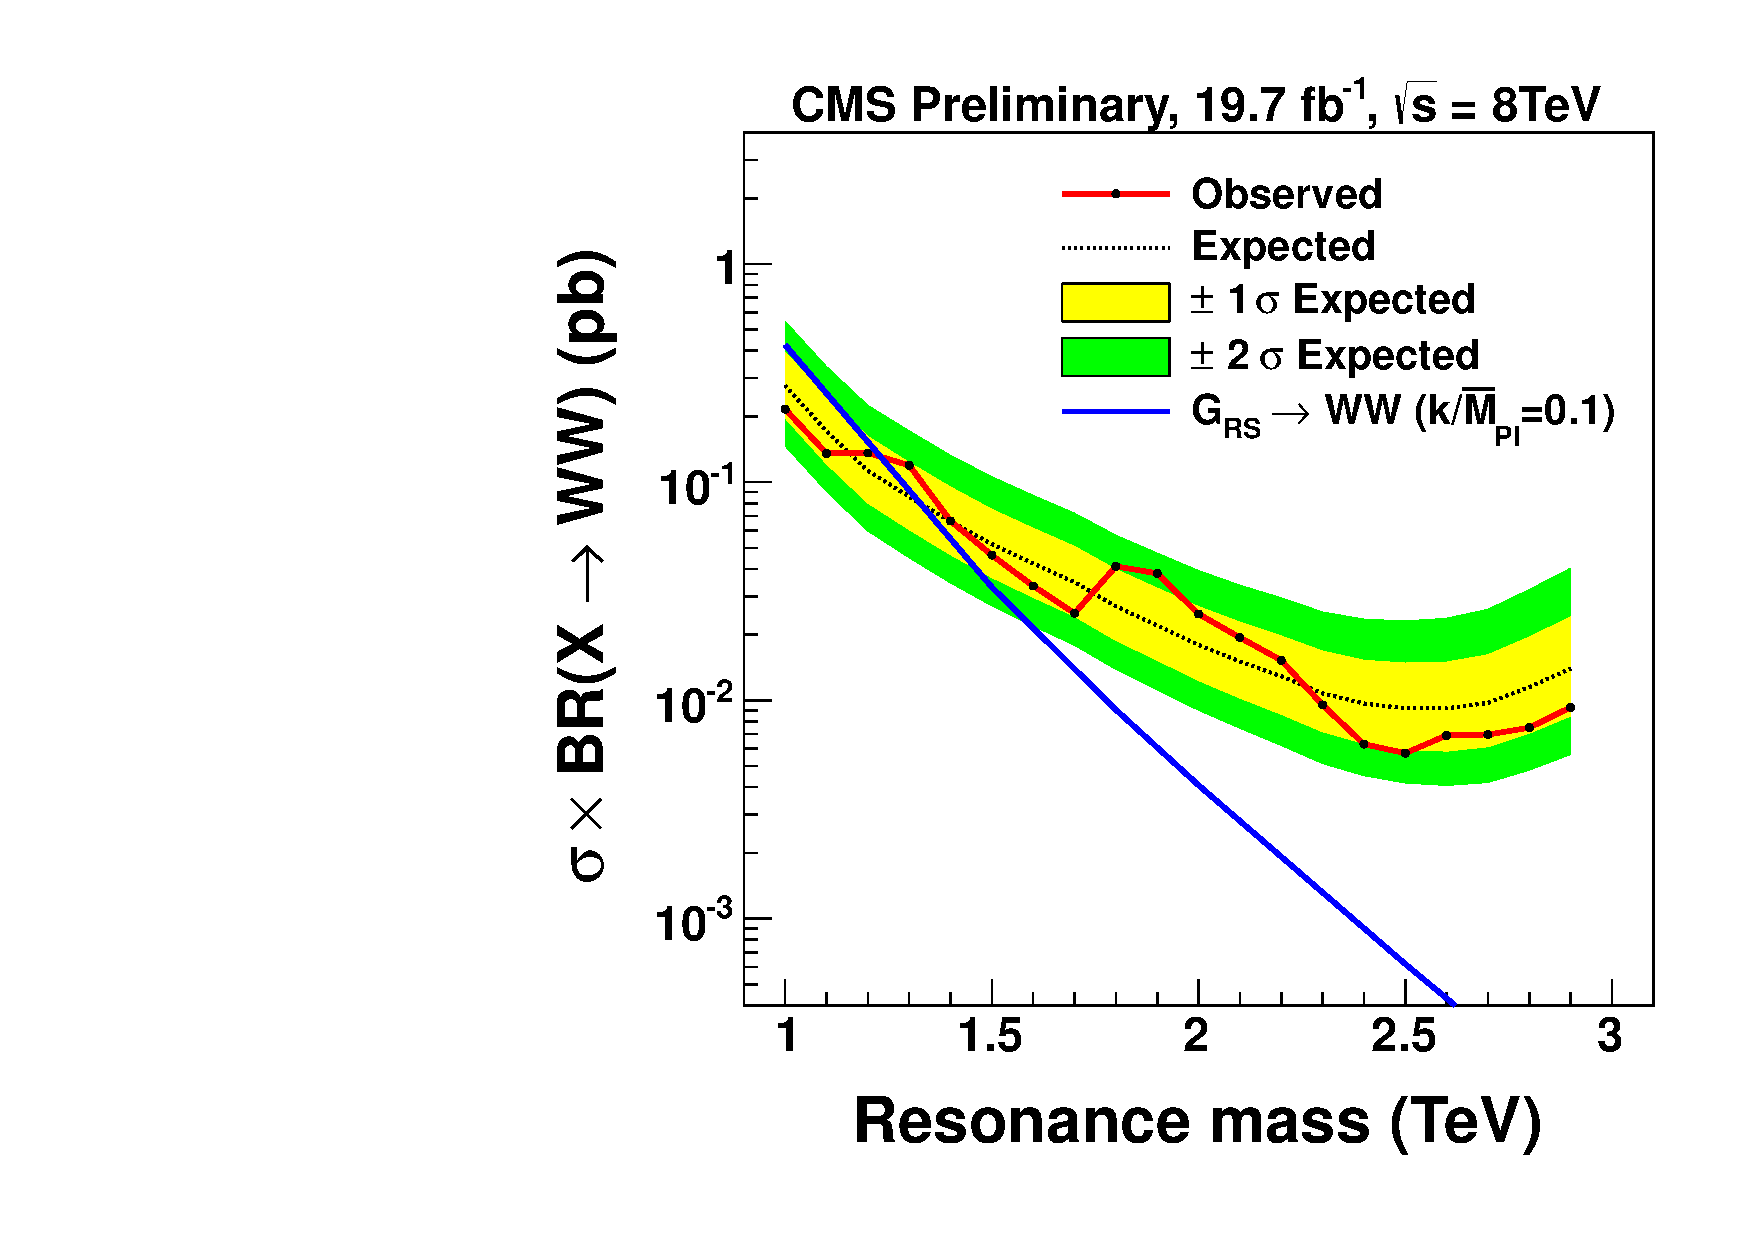
\includegraphics[width=0.35\textwidth]{figs/limits/brazilianFlag_RS1WW_combined.pdf}
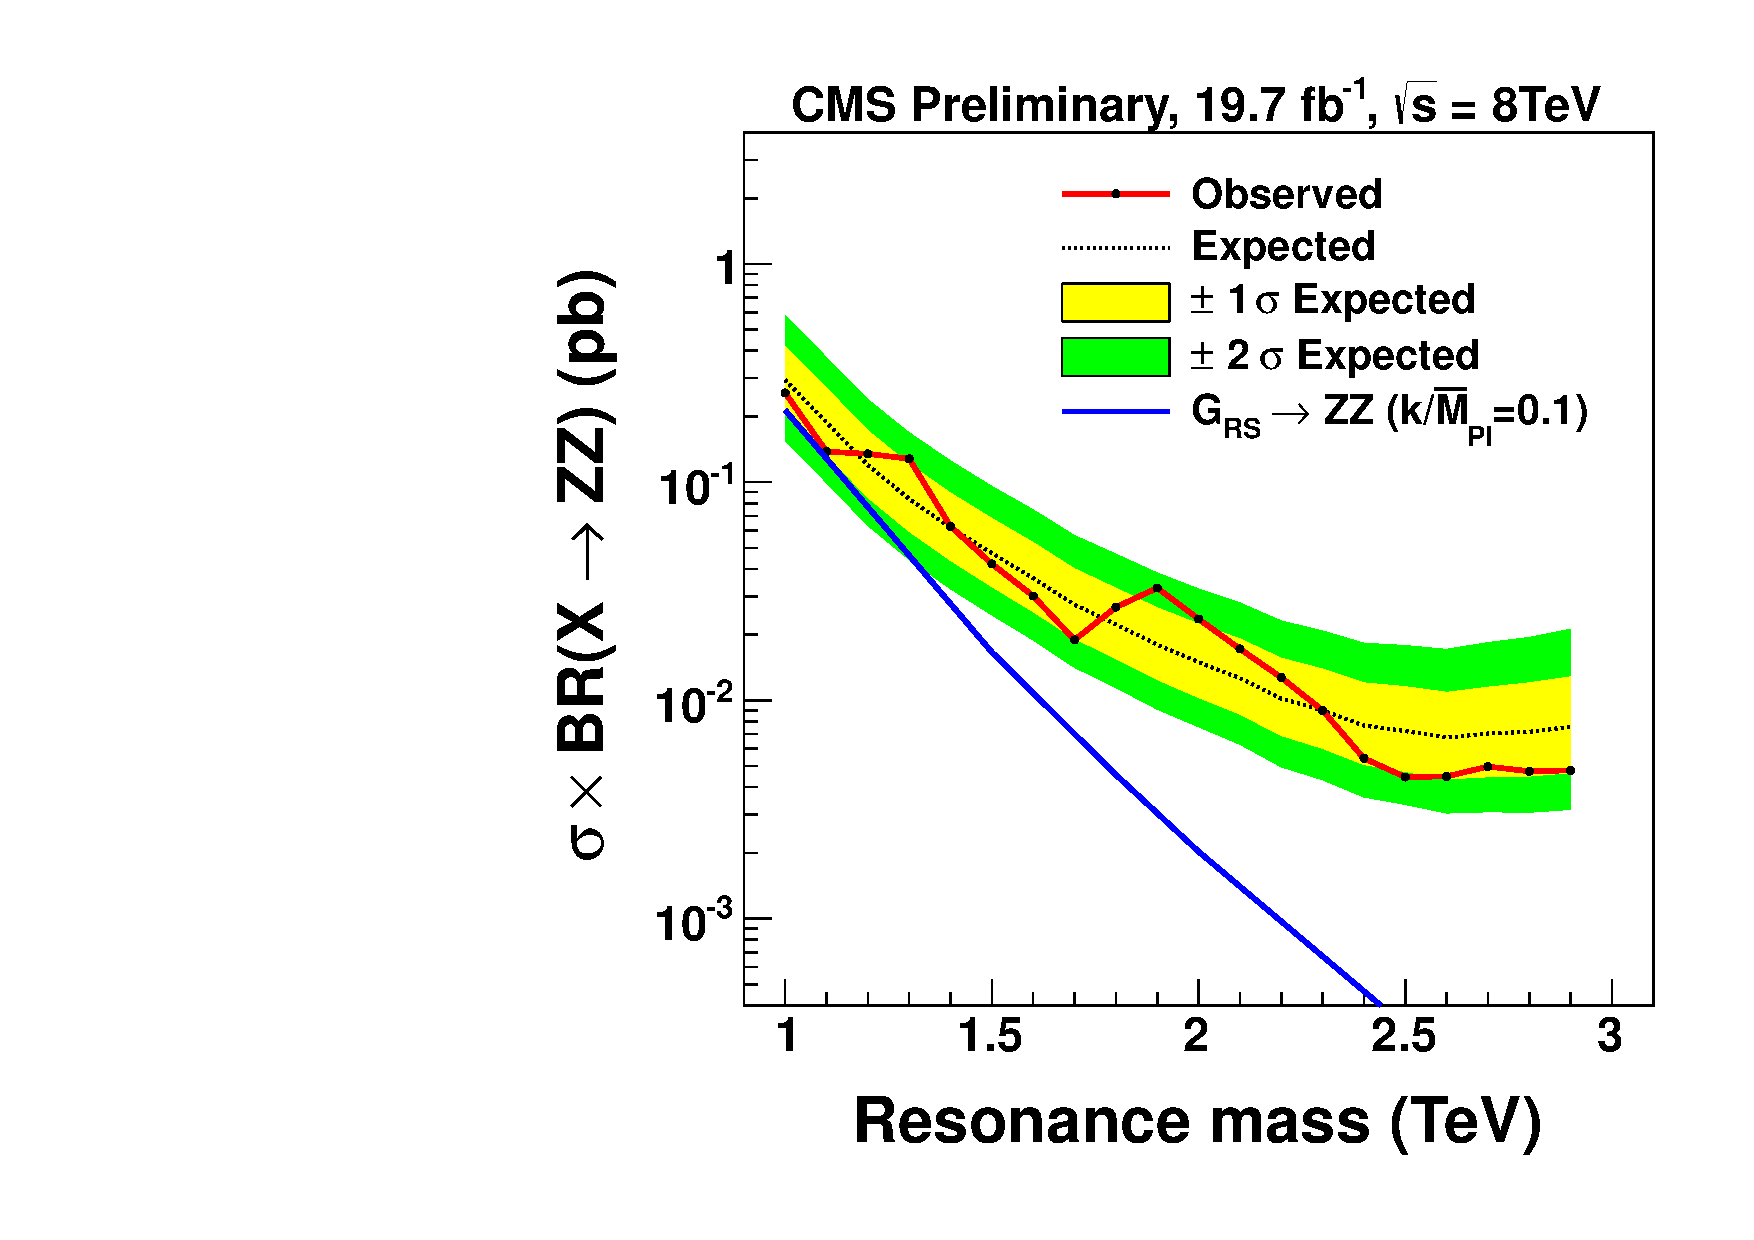
\includegraphics[width=0.35\textwidth]{figs/limits/brazilianFlag_RS1ZZ_combined.pdf}\\
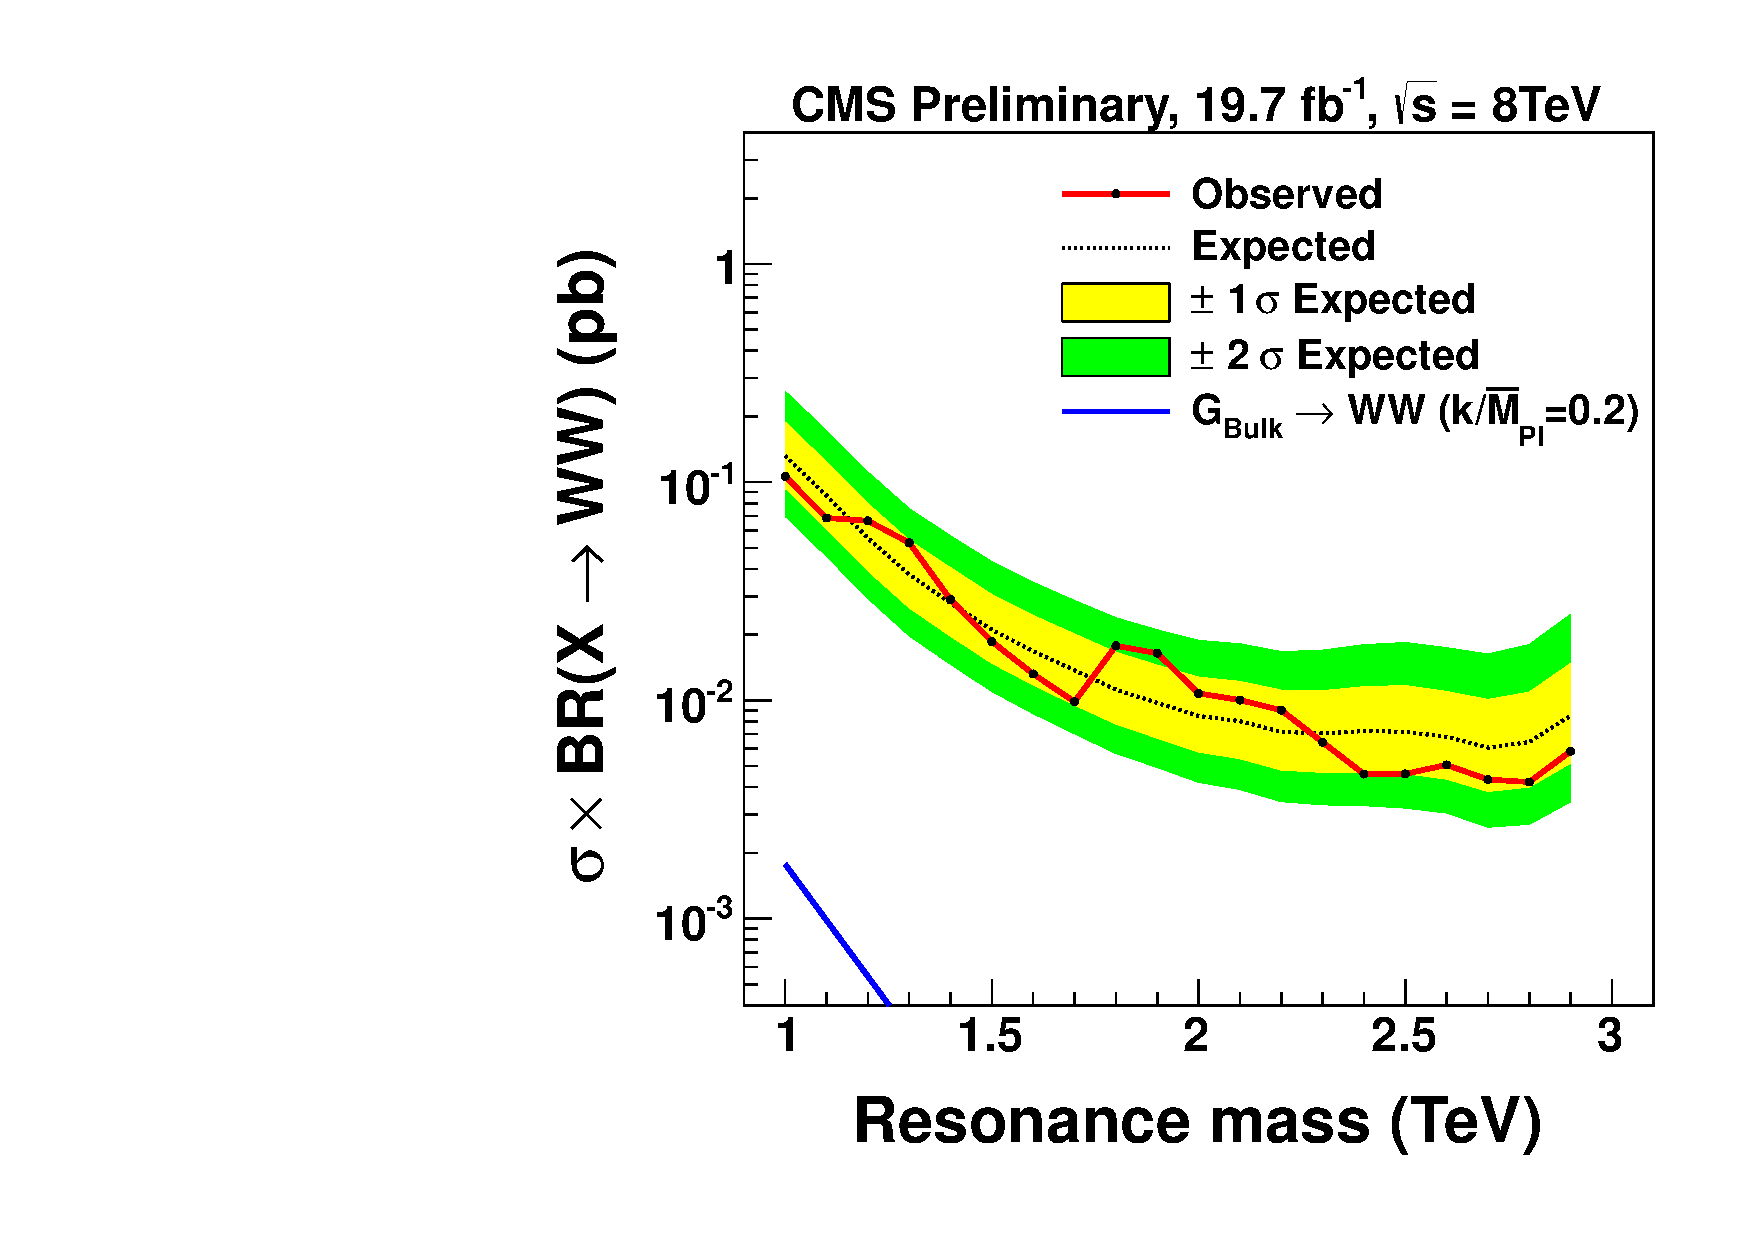
\includegraphics[width=0.35\textwidth]{figs/limits/brazilianFlag_BulkWW_combined.pdf}
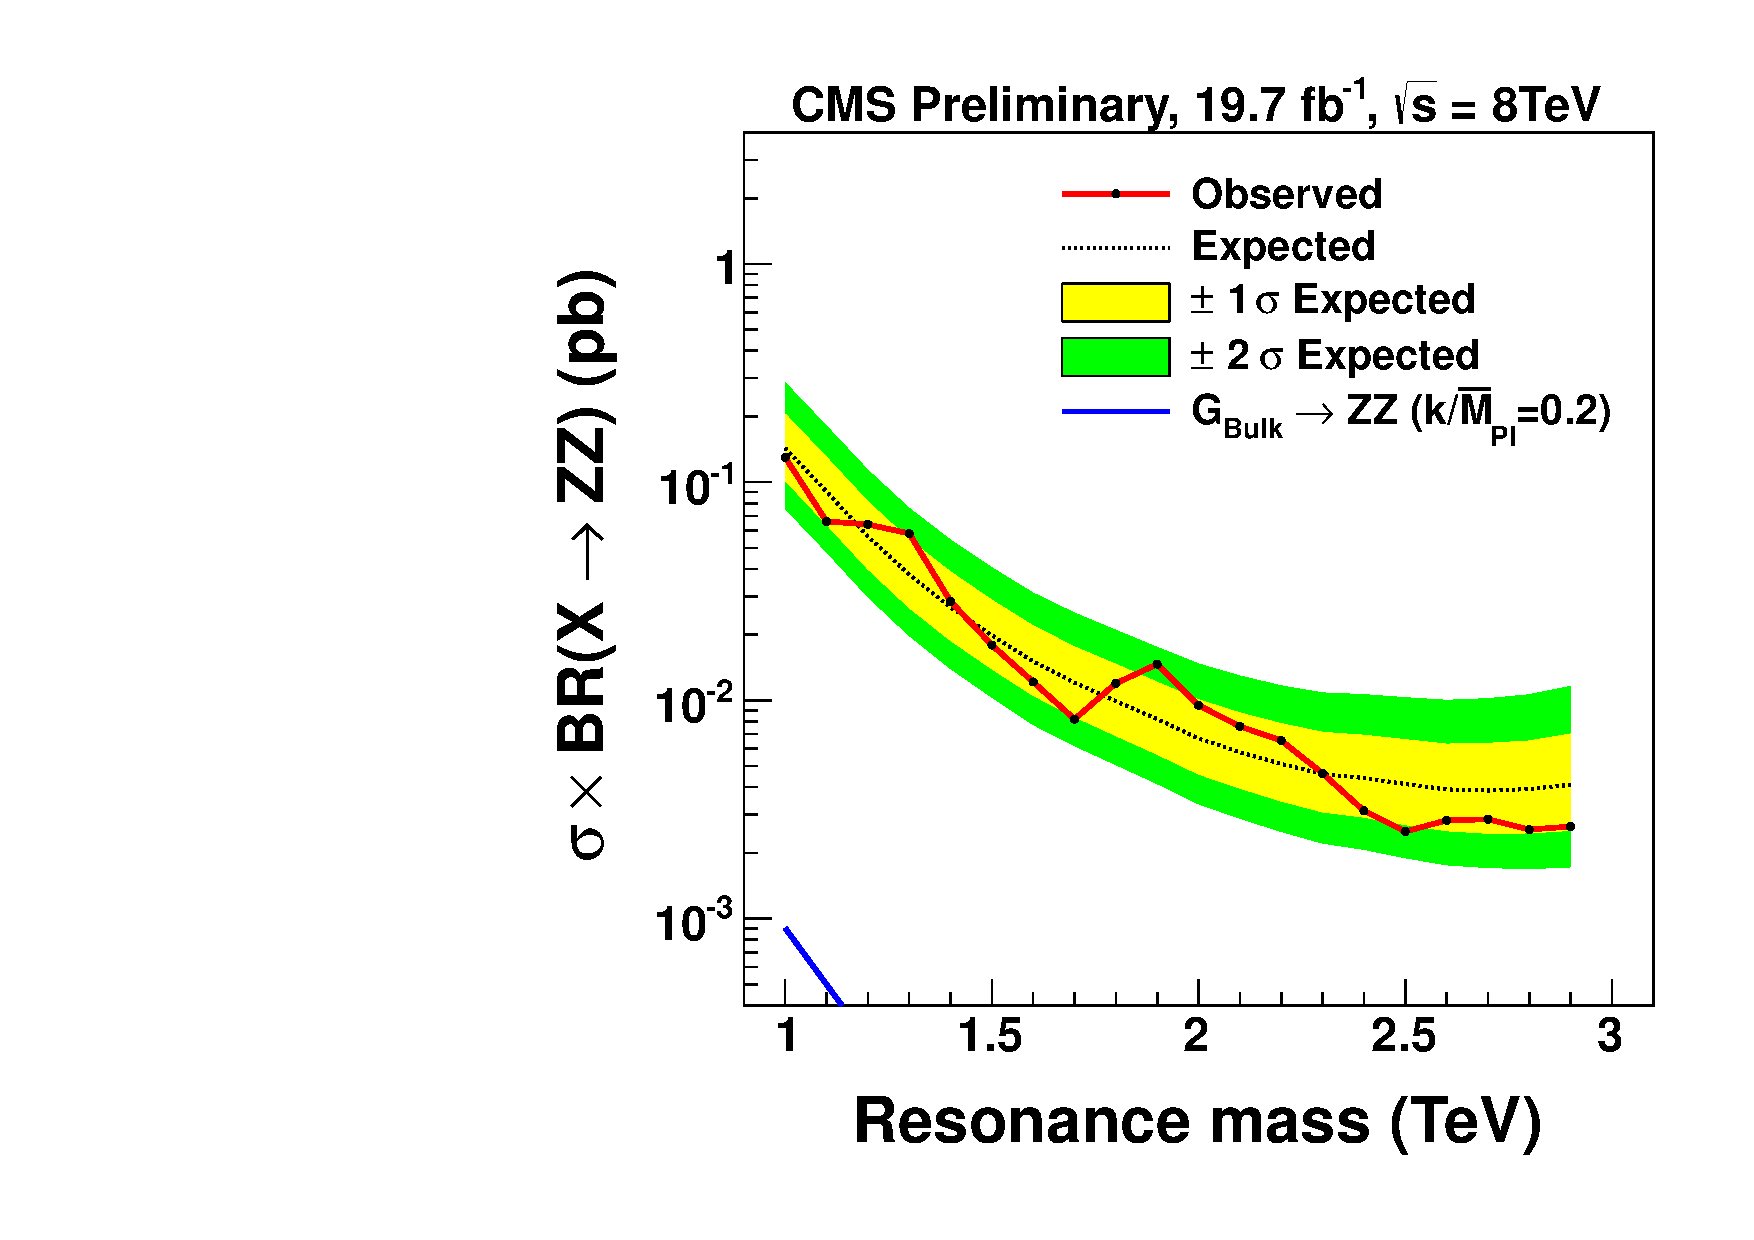
\includegraphics[width=0.35\textwidth]{figs/limits/brazilianFlag_BulkZZ_combined.pdf}\\
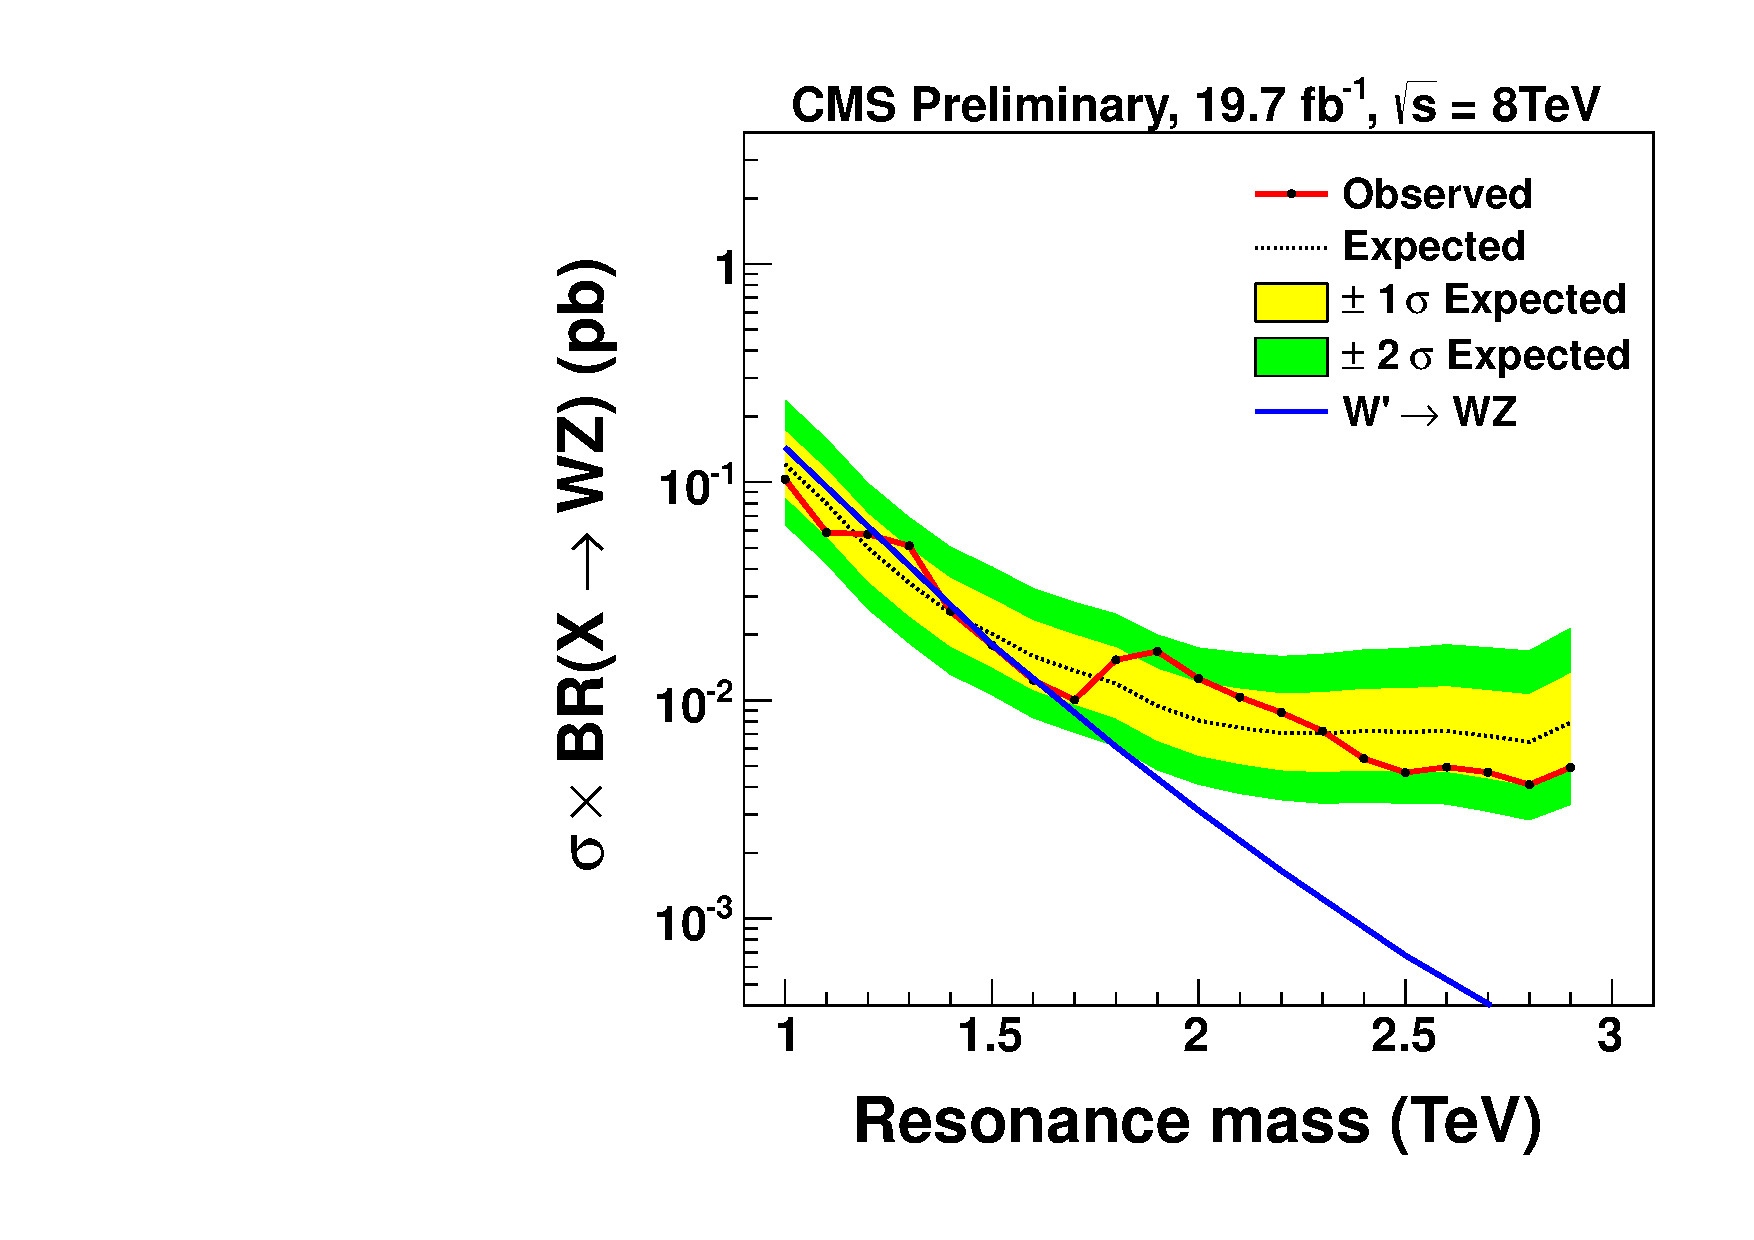
\includegraphics[width=0.35\textwidth]{figs/limits/brazilianFlag_WZ_combined.pdf}
\end{center}
\caption{Expected and observed limits for qW (top-left), qZ (top-right), \GRS WW (center-left), \GRS ZZ (center-right), \GBulk WW (center-left), \GBulk ZZ (center-right) and WZ (bottom) resonances
 combining the low-purity and high-purity categories.
  The predicted cross sections as a function of resonance mass for the considered benchmark models are overlaid.}
\label{fig:Vtagresults3}
\end{figure*}

\begin{figure*}[h!tpb]
\begin{center}
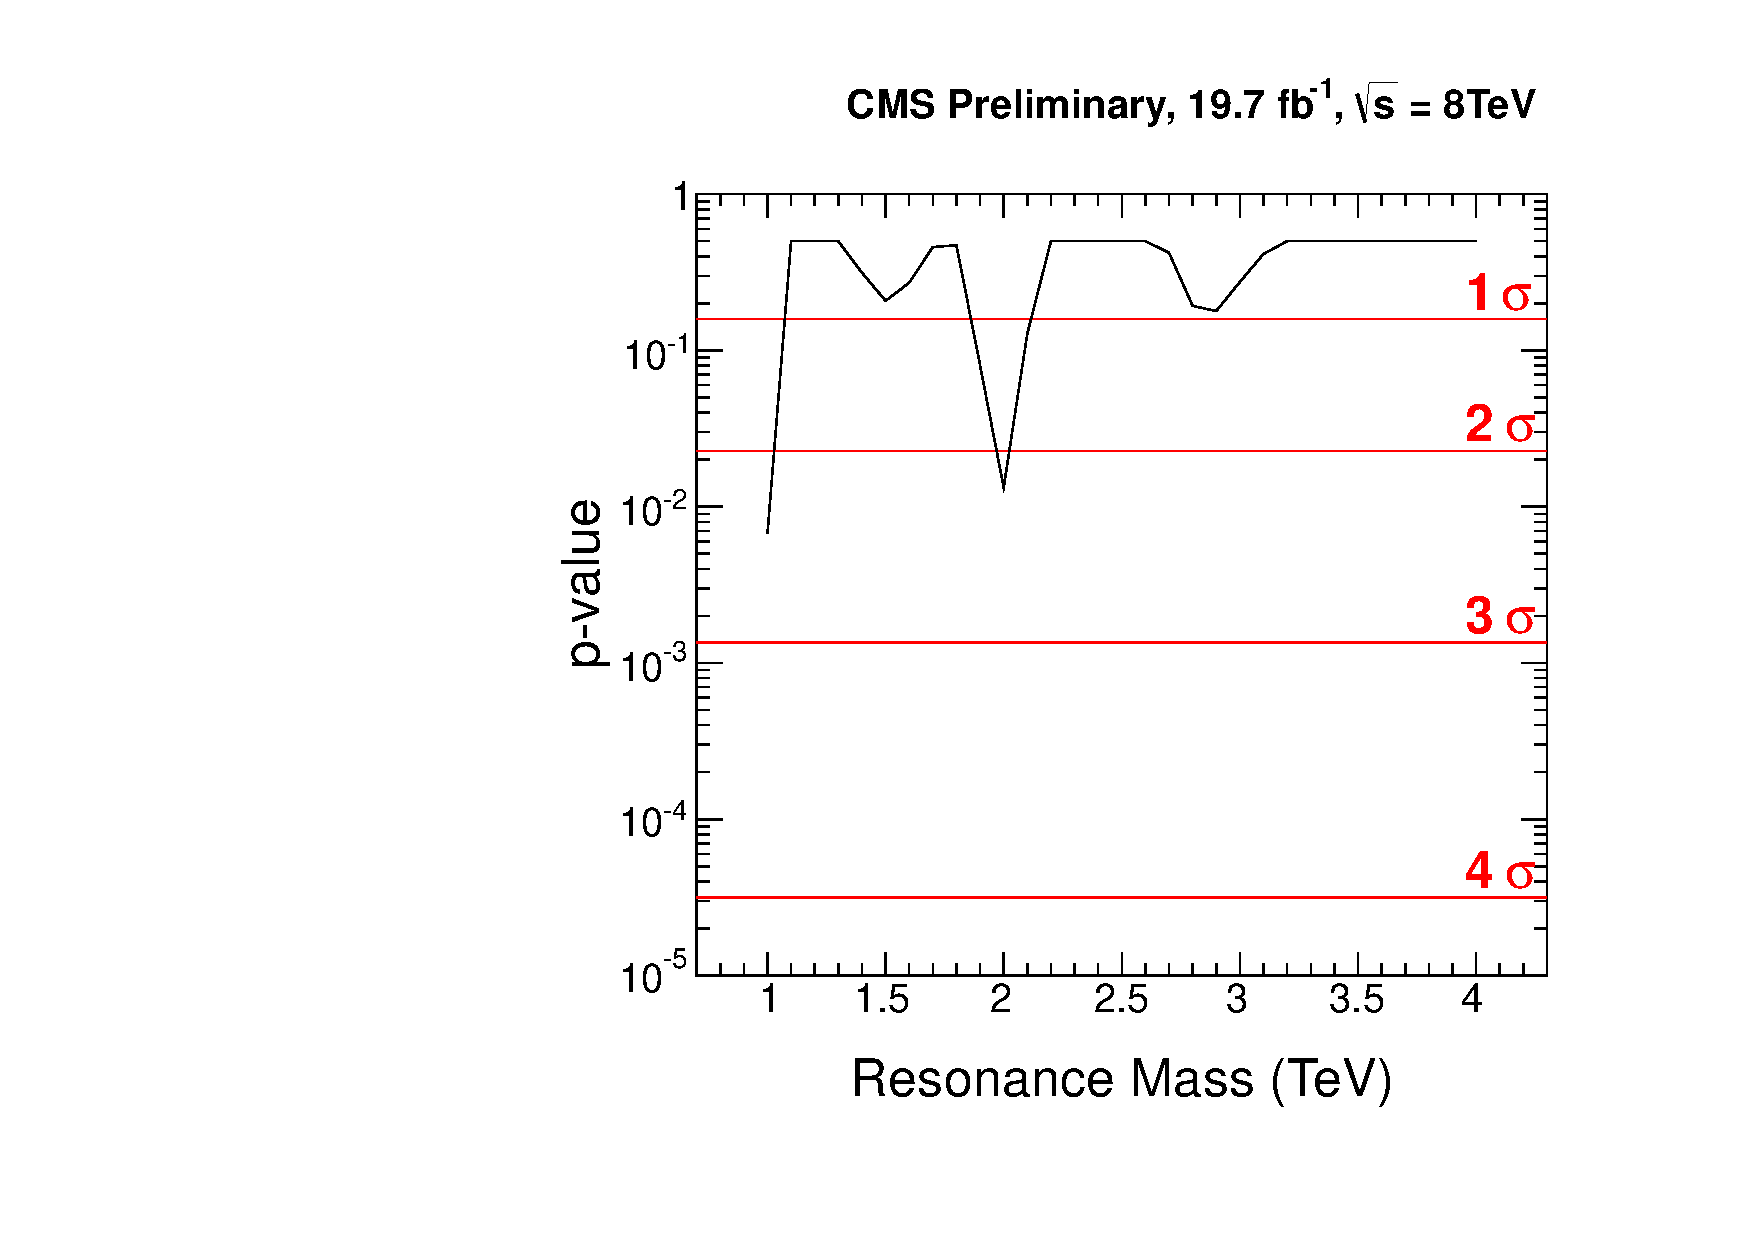
\includegraphics[width=0.35\textwidth]{figs/limits/pvalue_qW_low_purity.pdf}
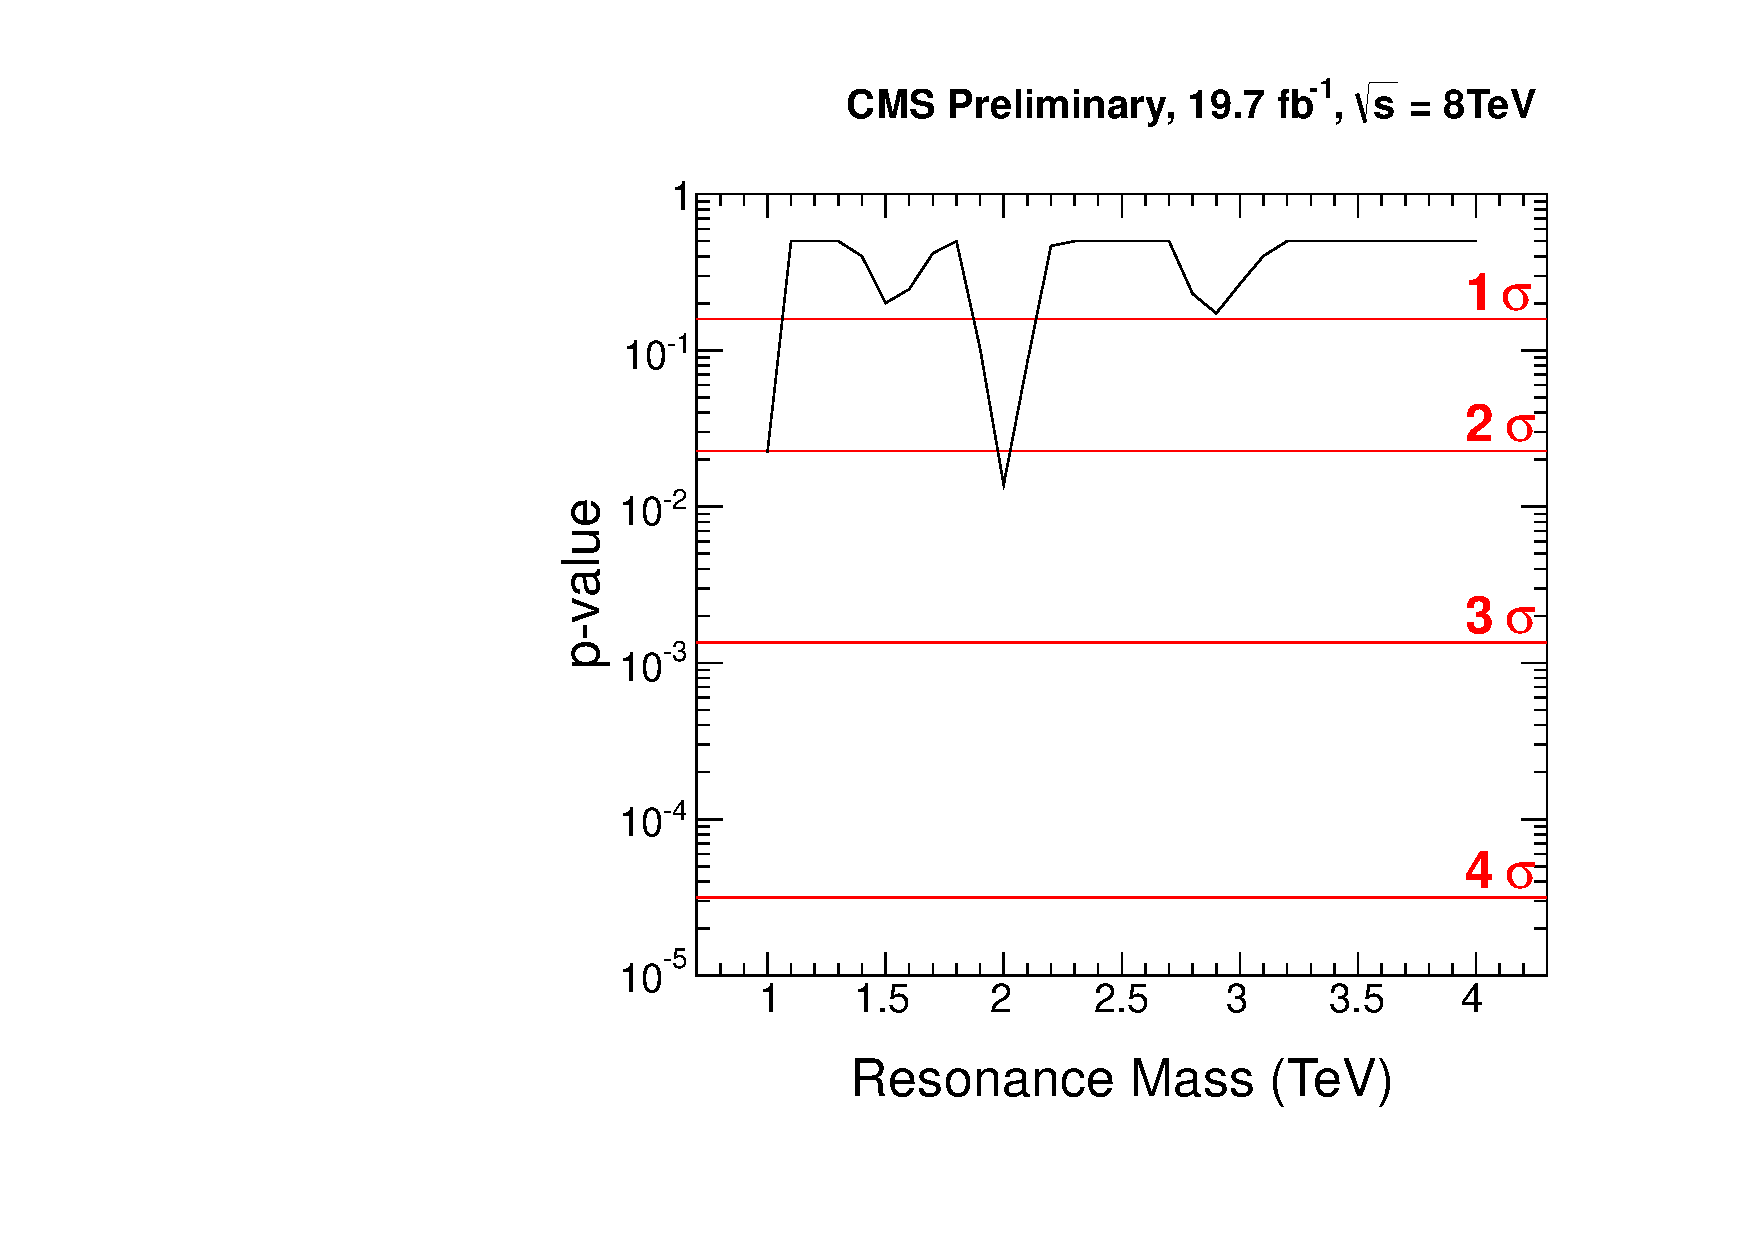
\includegraphics[width=0.35\textwidth]{figs/limits/pvalue_qZ_low_purity.pdf}\\
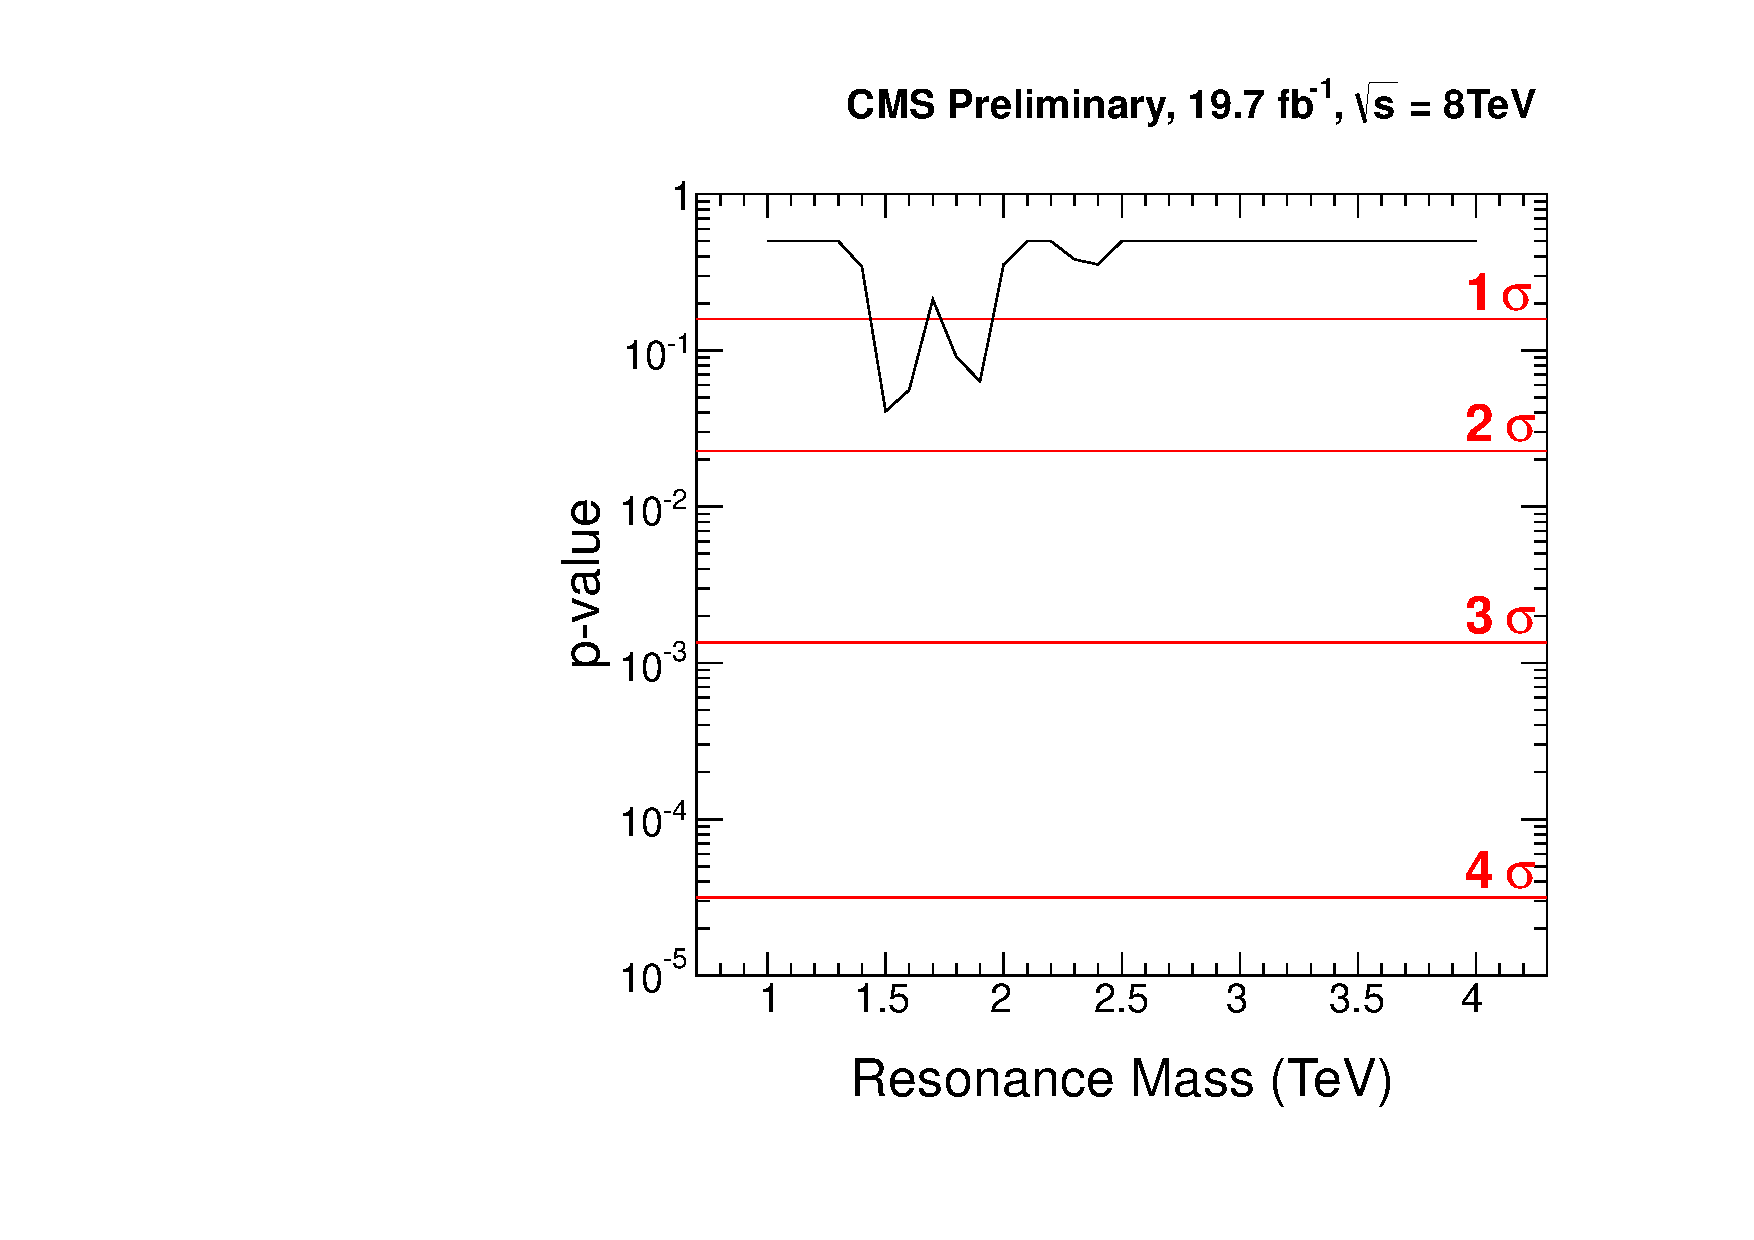
\includegraphics[width=0.35\textwidth]{figs/limits/pvalue_qW_high_purity.pdf}
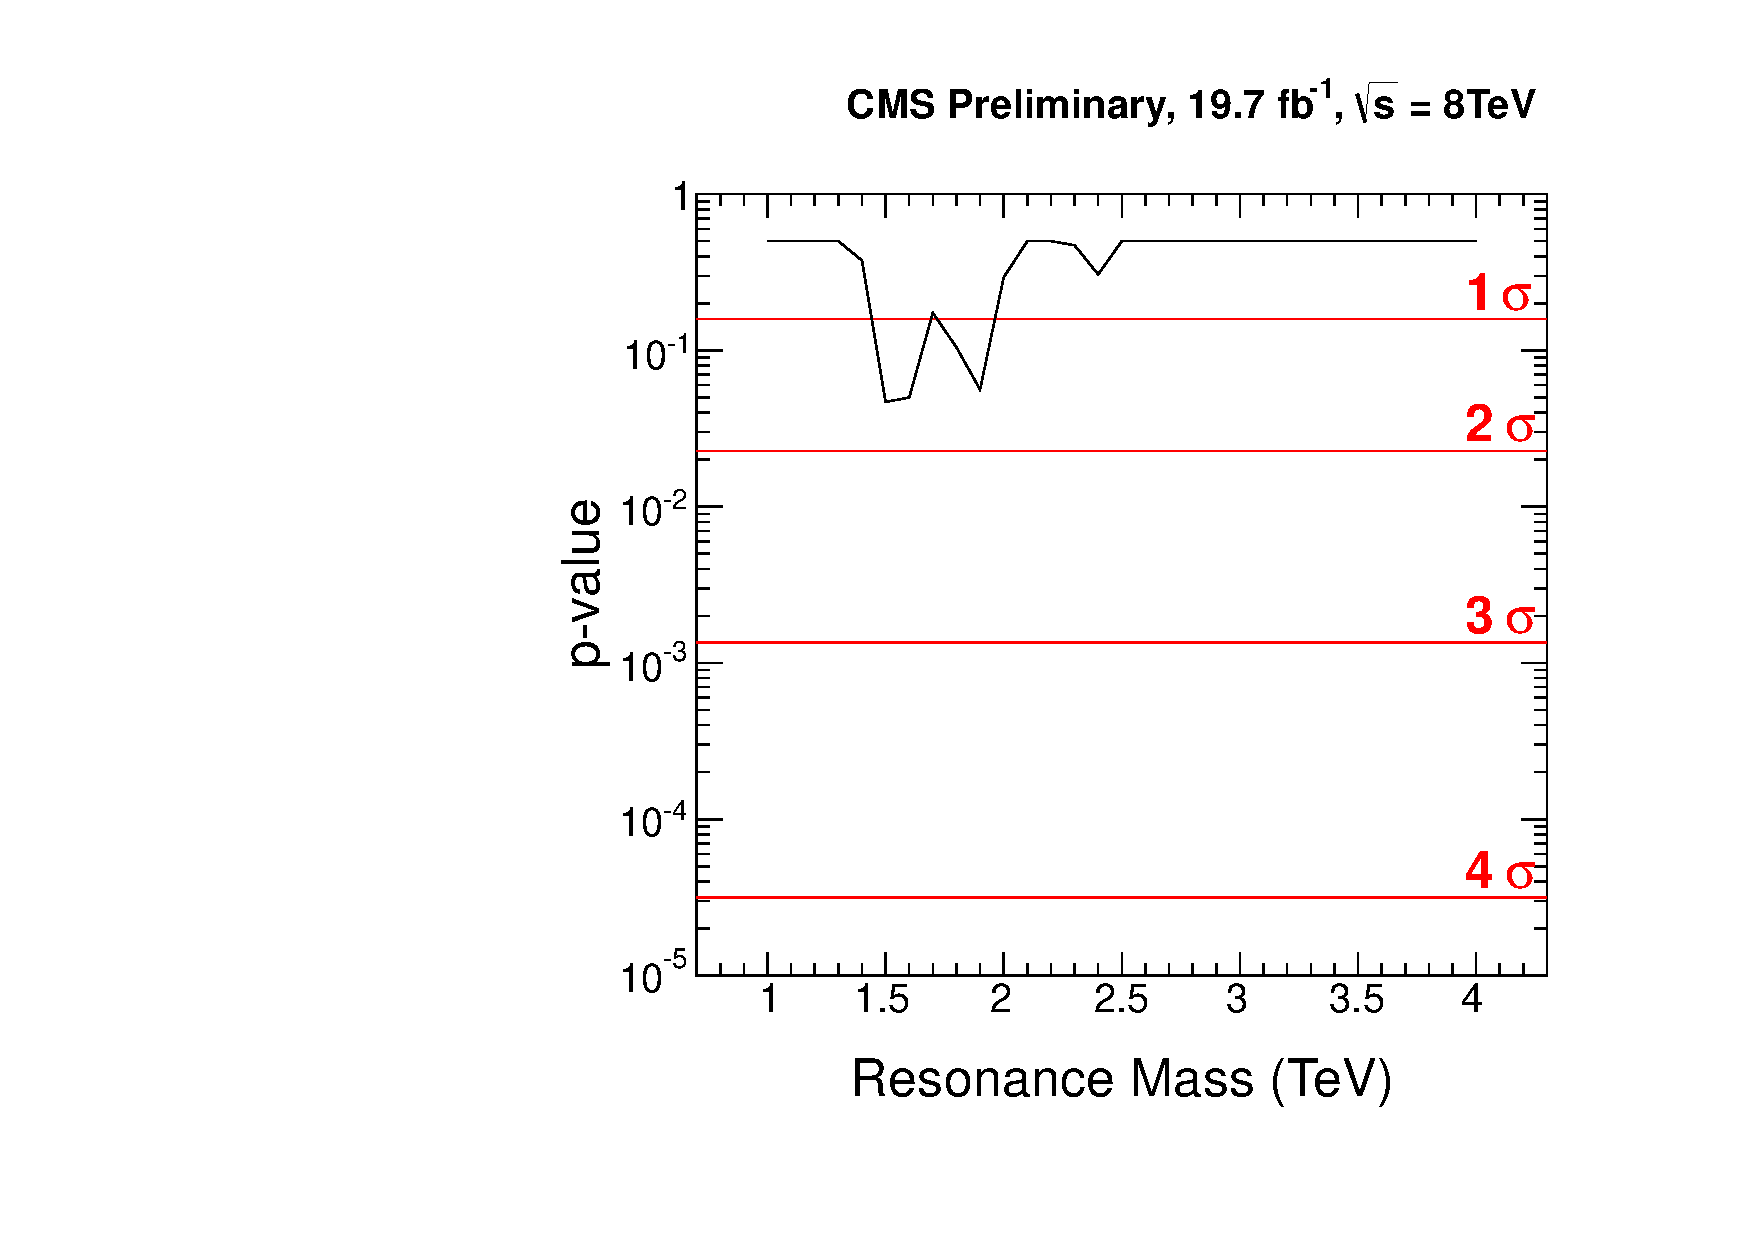
\includegraphics[width=0.35\textwidth]{figs/limits/pvalue_qZ_high_purity.pdf}\\
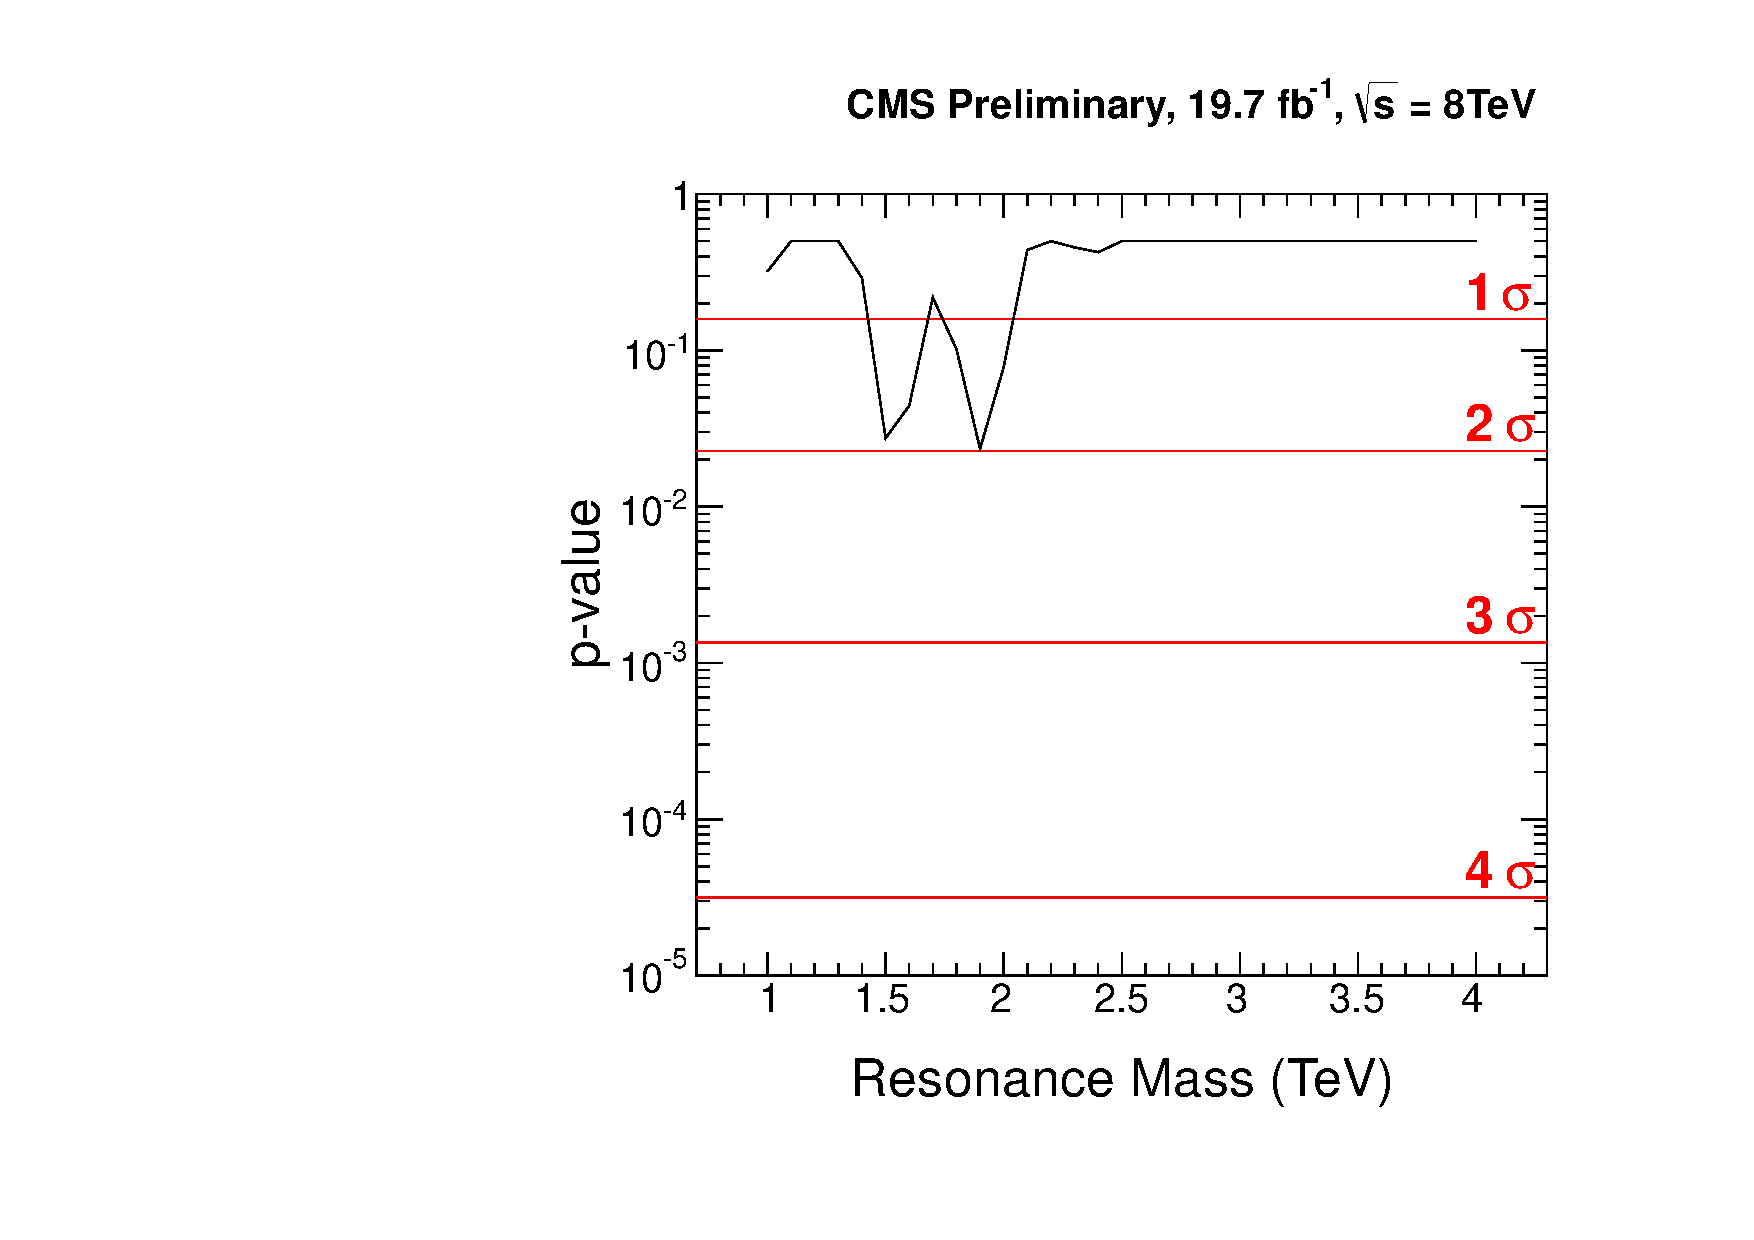
\includegraphics[width=0.35\textwidth]{figs/limits/pvalue_qW_combined.pdf}
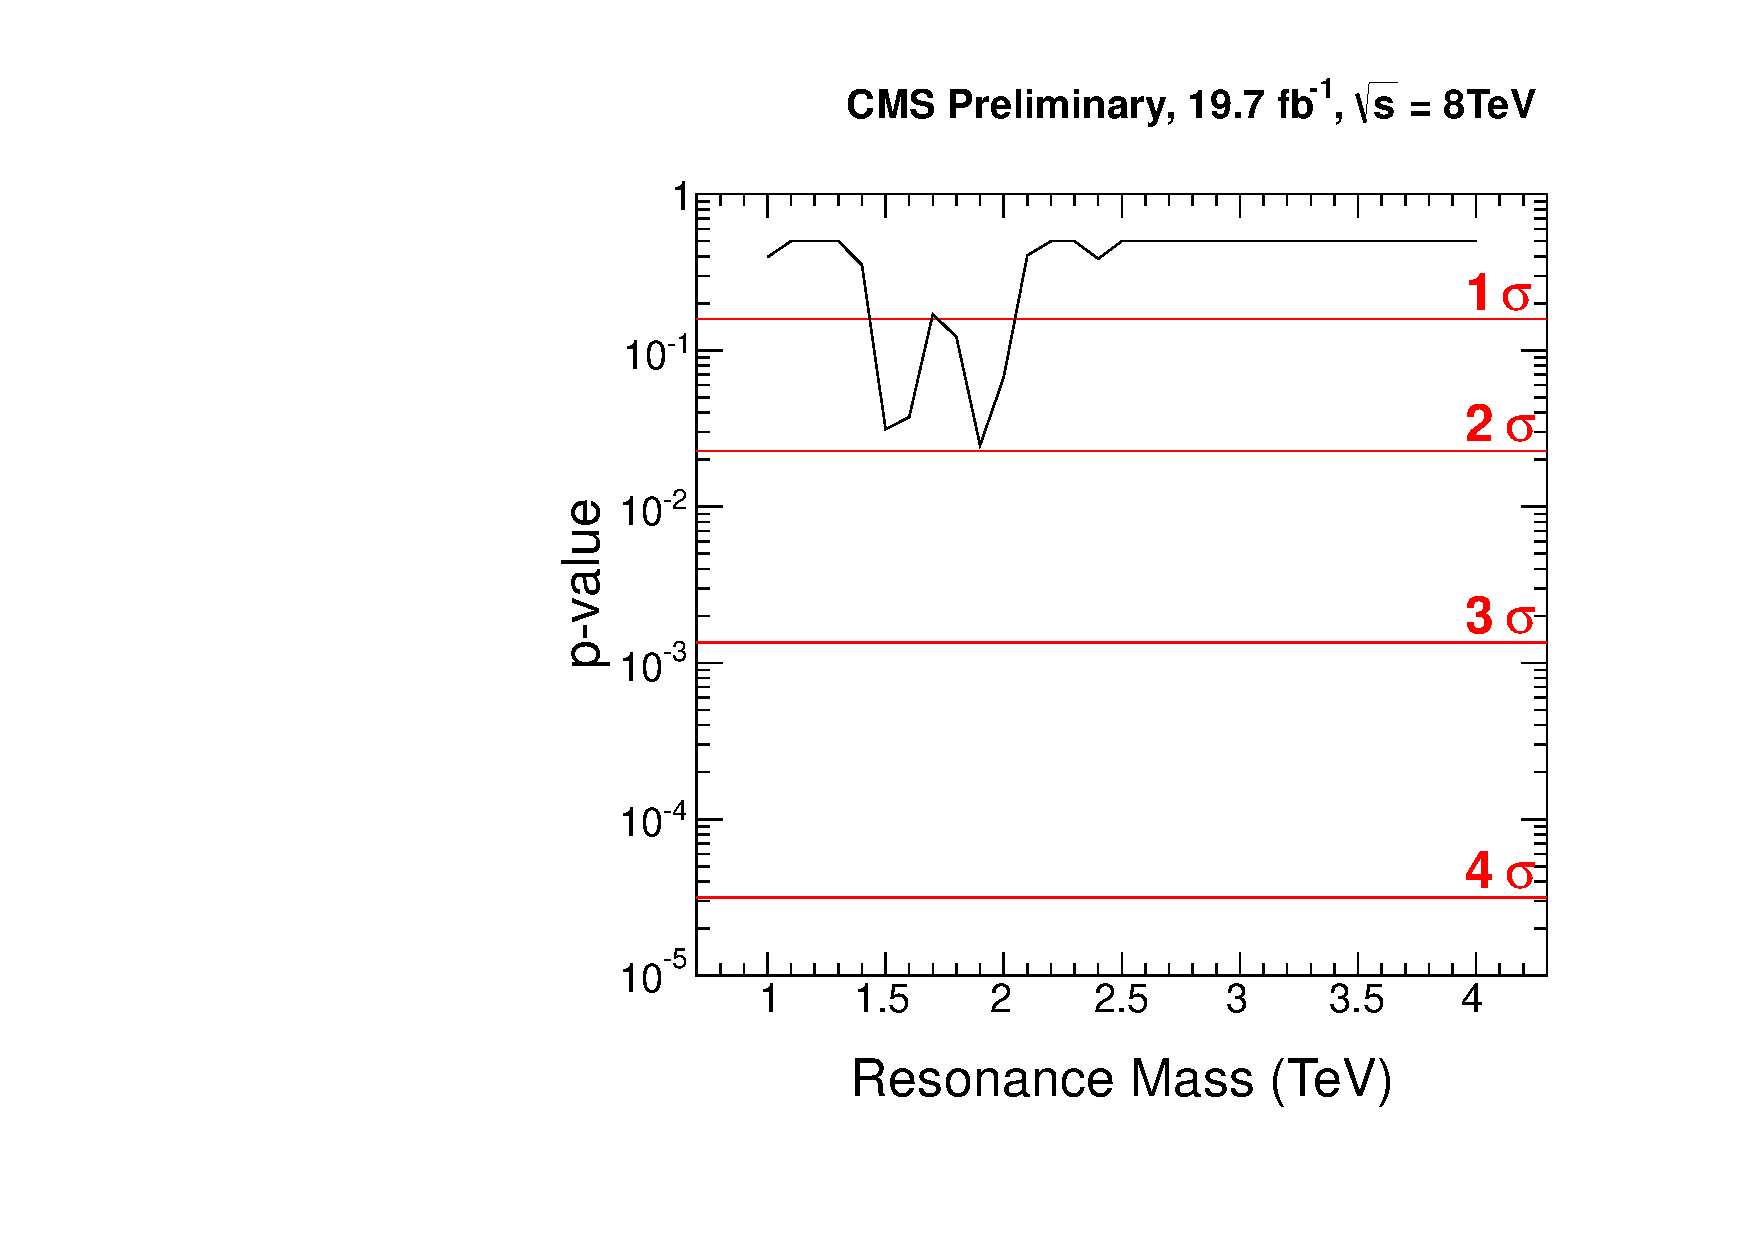
\includegraphics[width=0.35\textwidth]{figs/limits/pvalue_qZ_combined.pdf}
\end{center}
\caption{Observed local p-values assuming a qW (left) and qZ (right) signal model in the singly-tagged dijet mass spectrum in the low-purity (top), high-purity (middle) and combination (botton).}
\label{fig:Vtagresults4}
\end{figure*}

\begin{figure*}[h!tpb]
\begin{center}
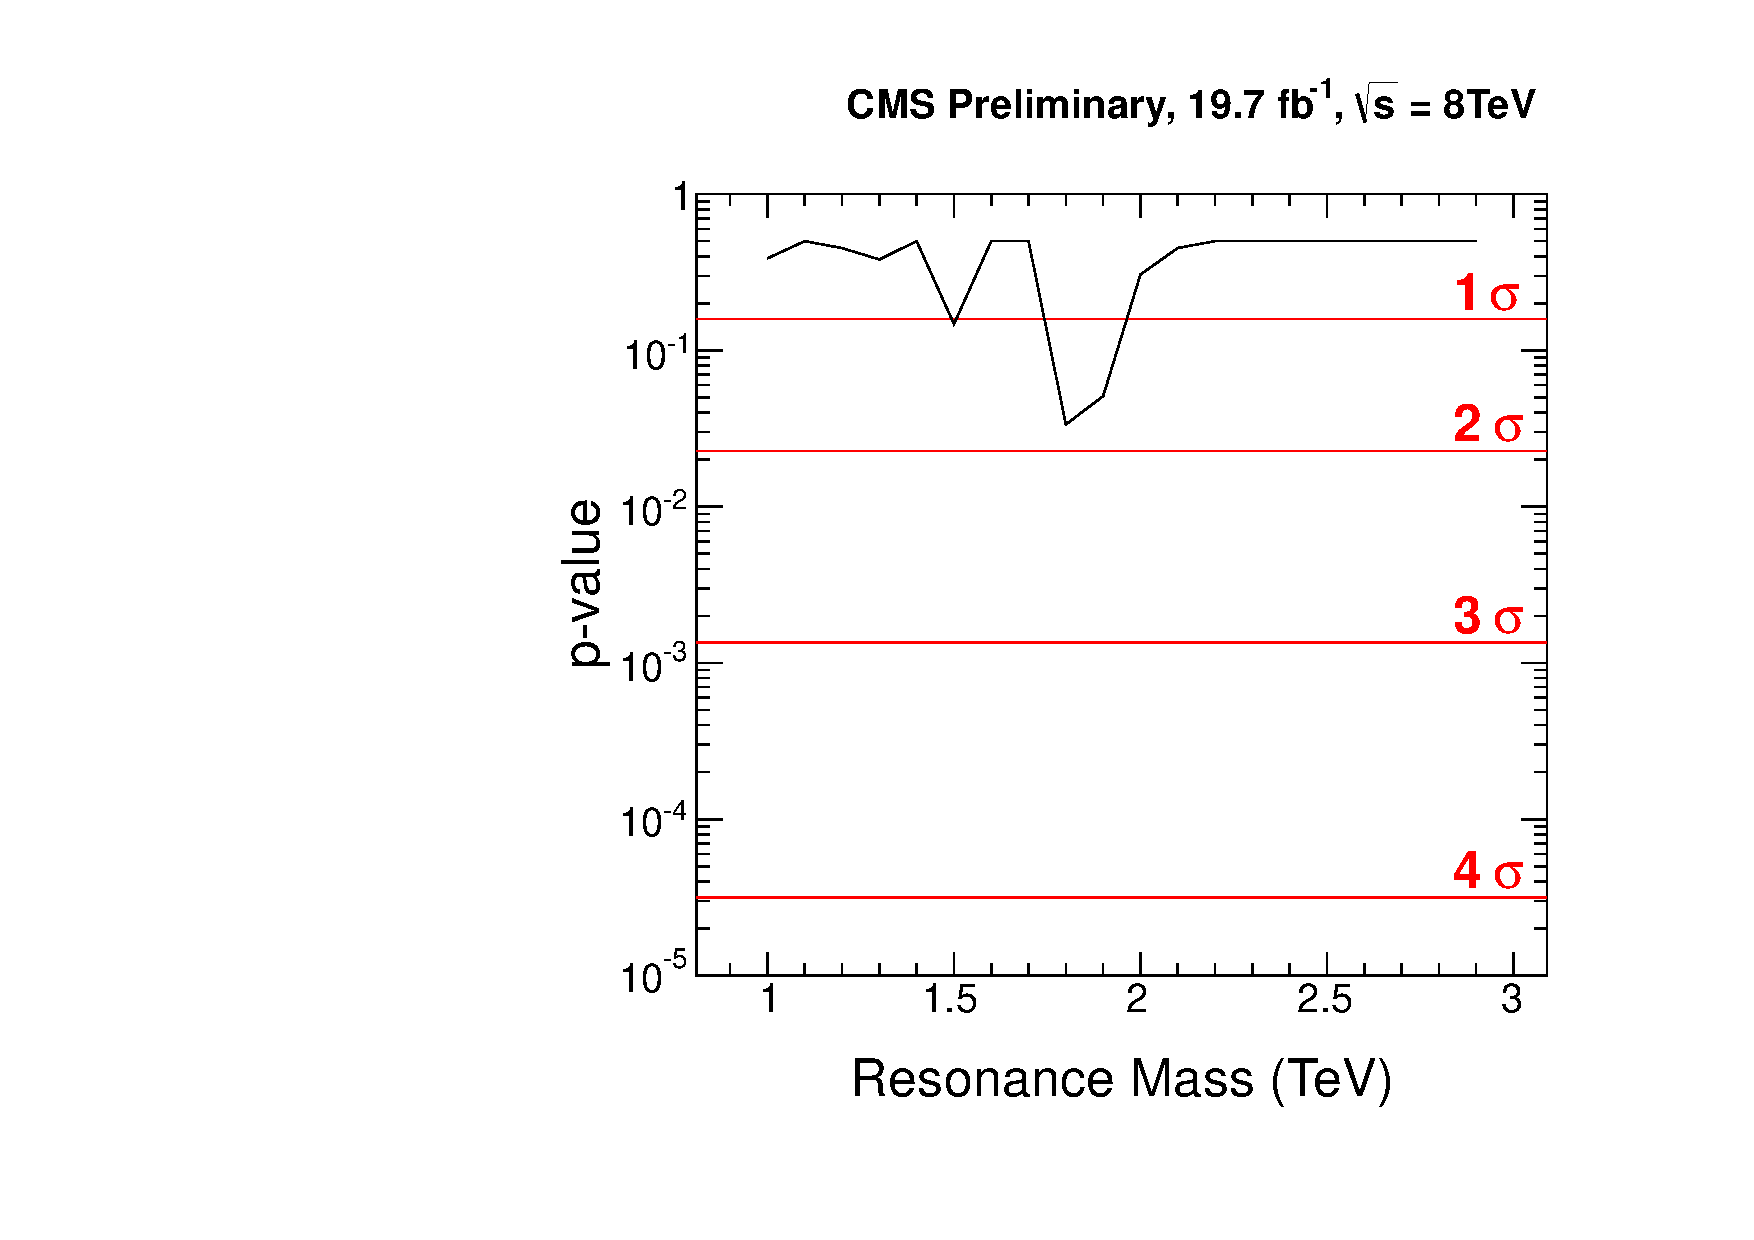
\includegraphics[width=0.35\textwidth]{figs/limits/pvalue_RS1WW_low_purity.pdf}
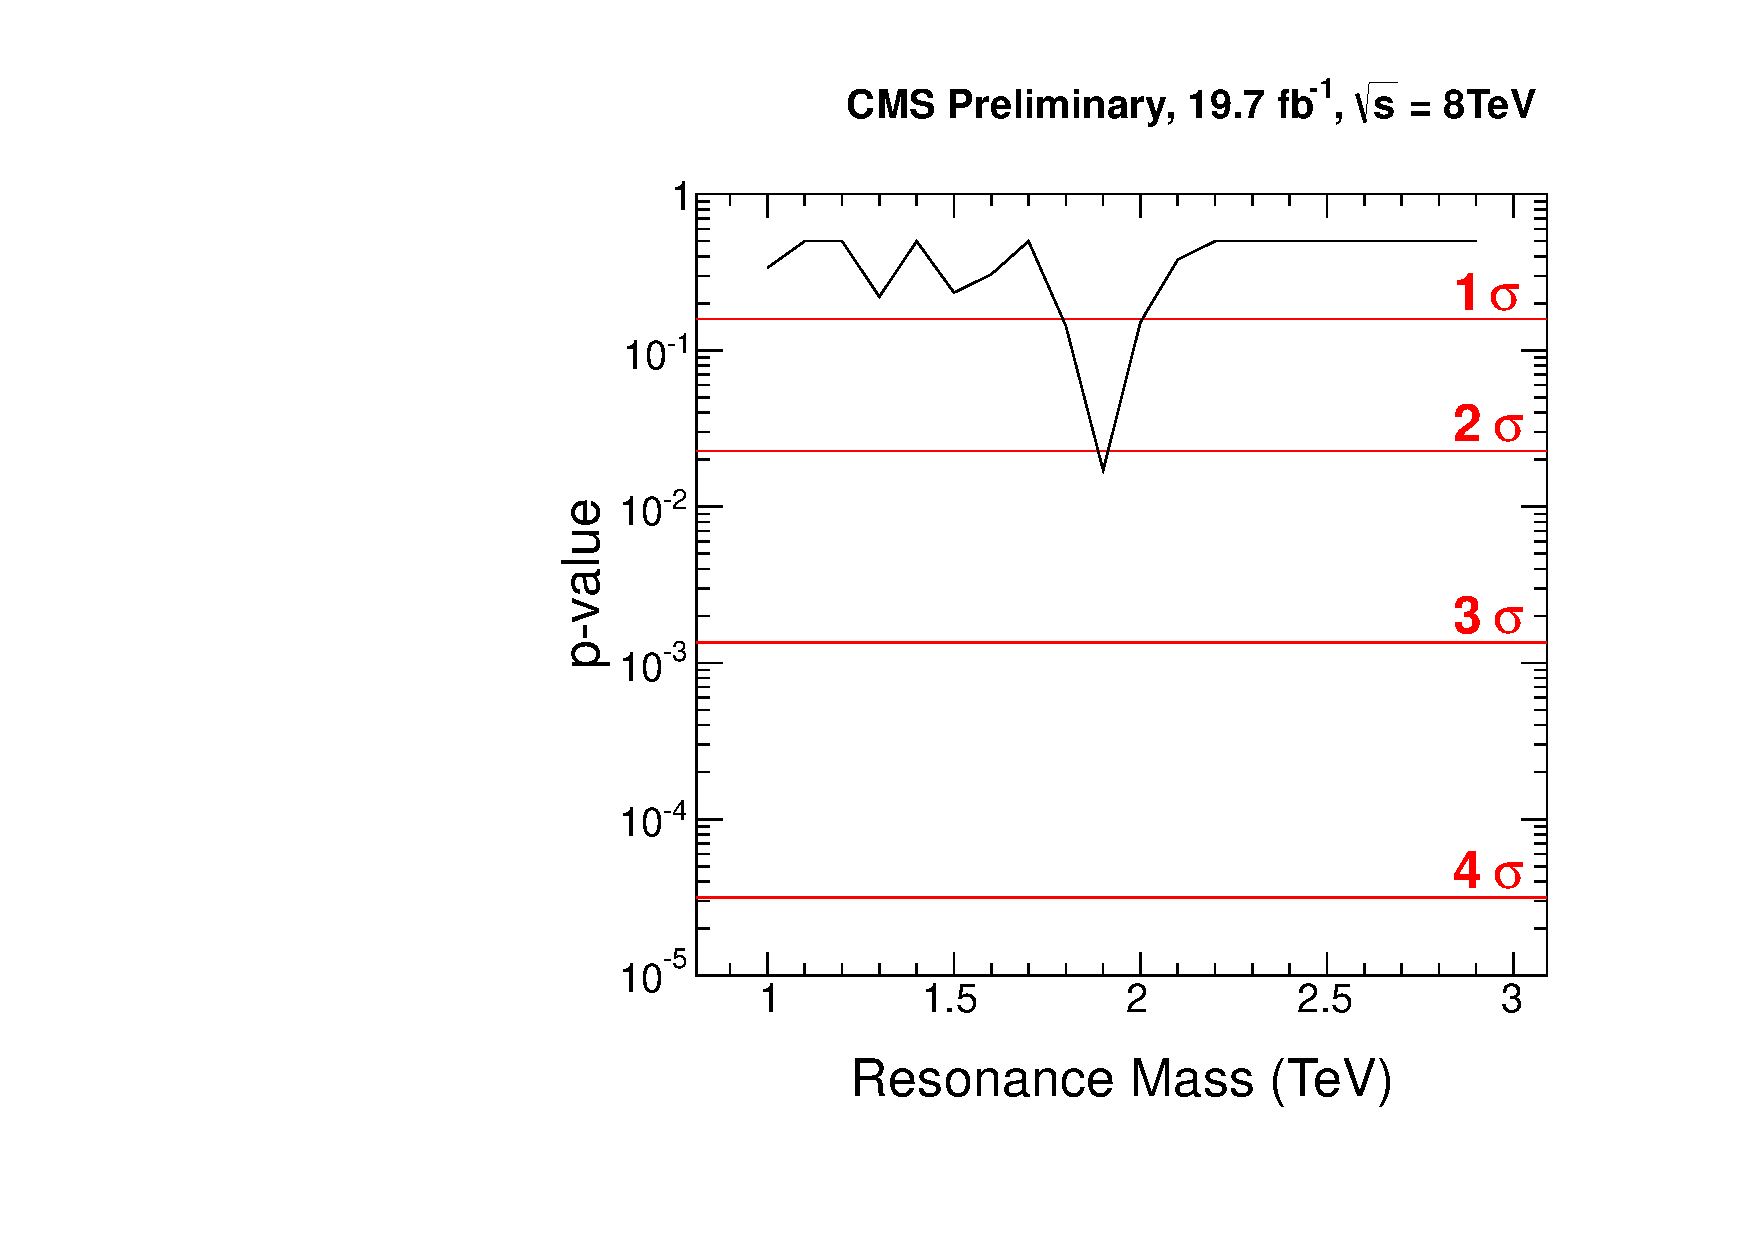
\includegraphics[width=0.35\textwidth]{figs/limits/pvalue_RS1ZZ_low_purity.pdf}\\
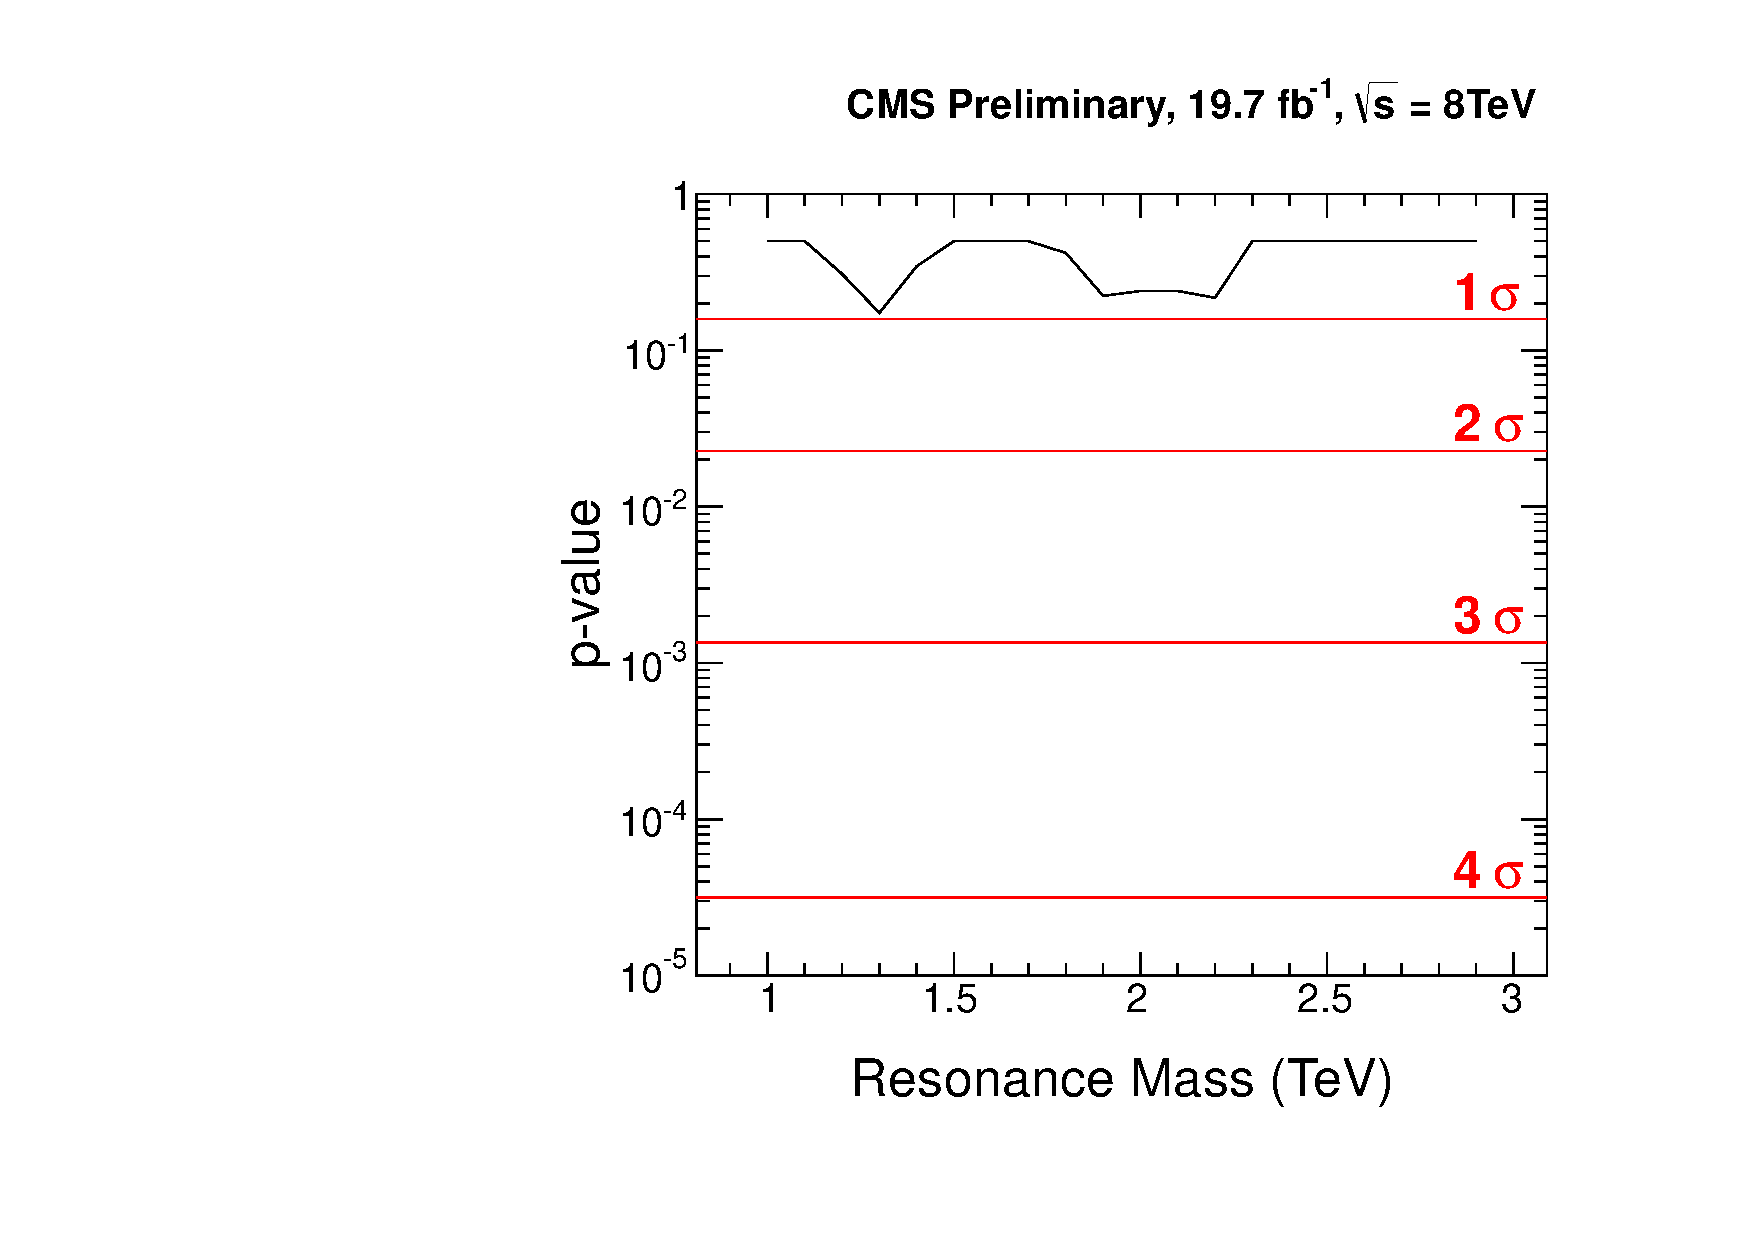
\includegraphics[width=0.35\textwidth]{figs/limits/pvalue_RS1WW_high_purity.pdf}
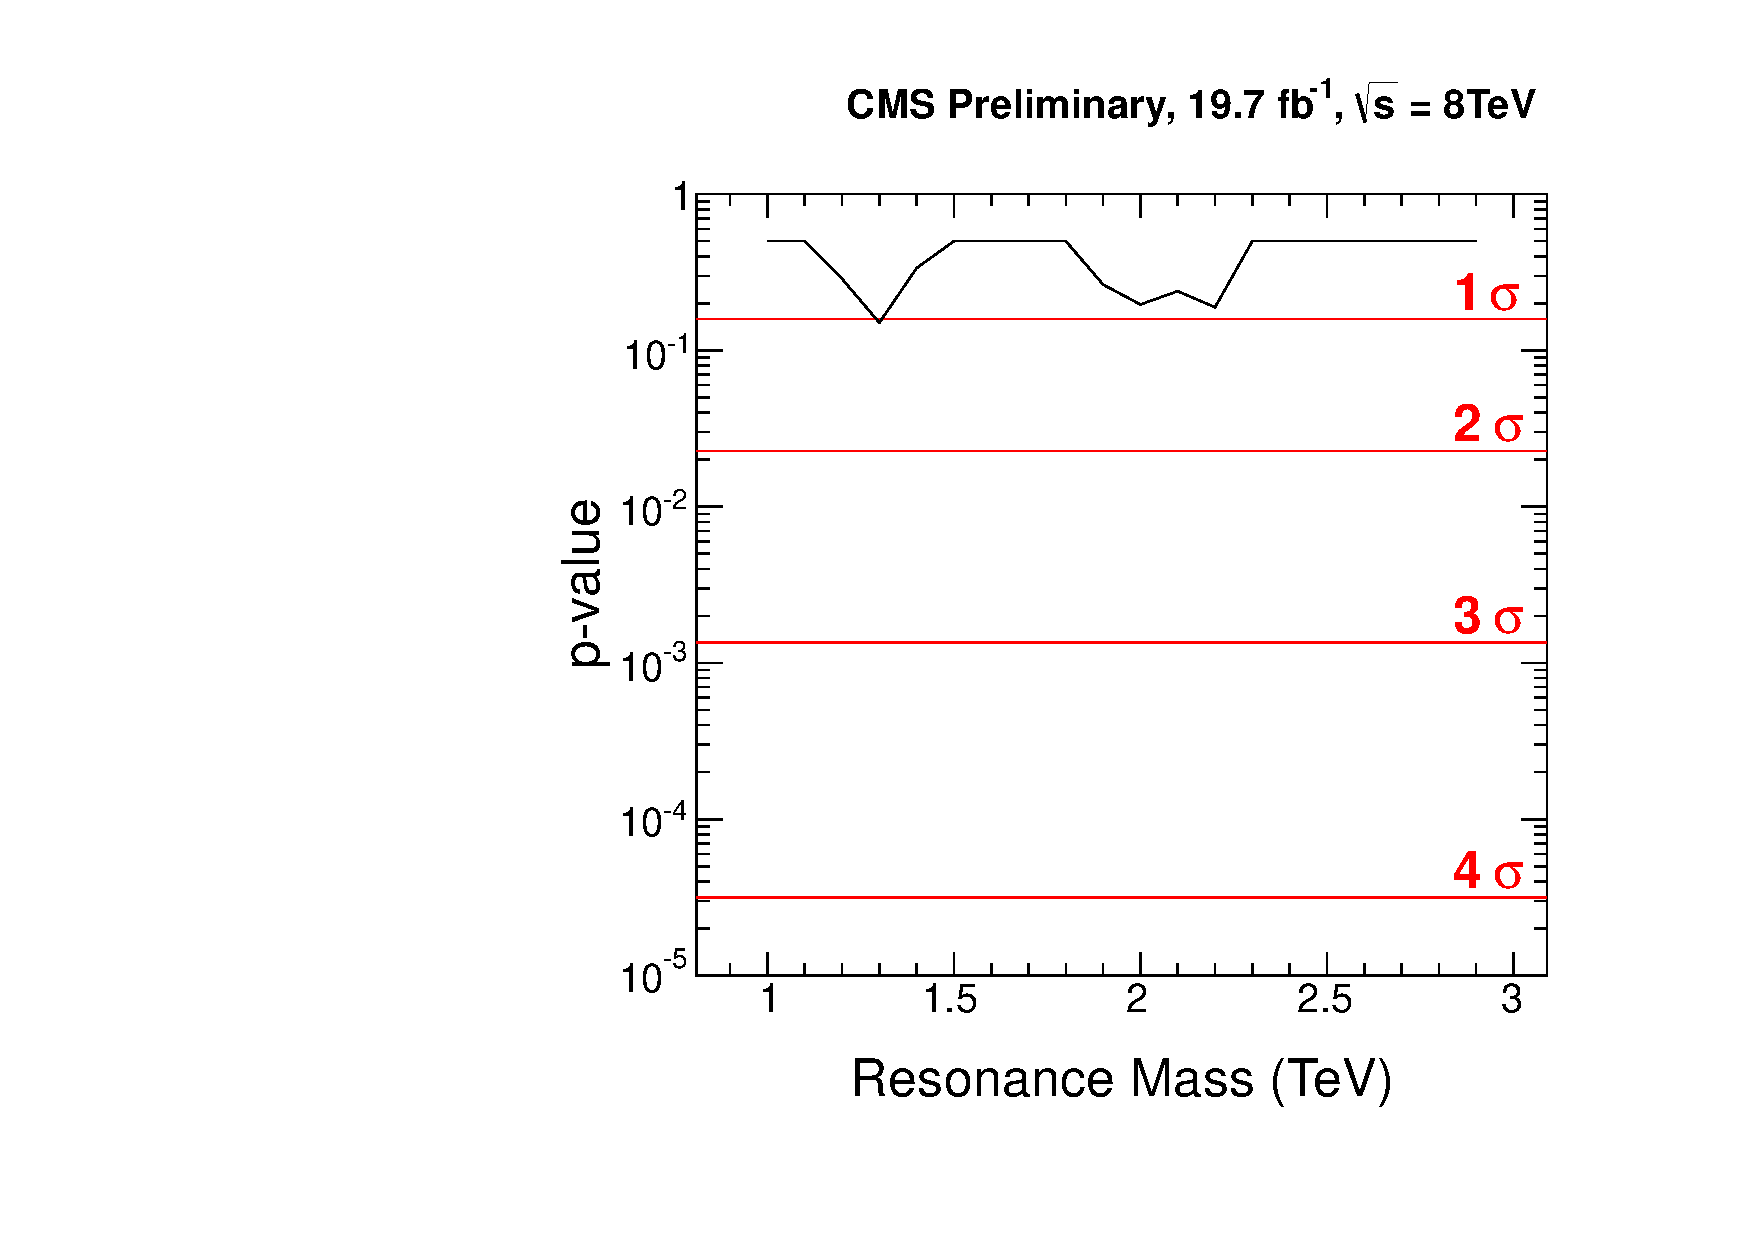
\includegraphics[width=0.35\textwidth]{figs/limits/pvalue_RS1ZZ_high_purity.pdf}\\
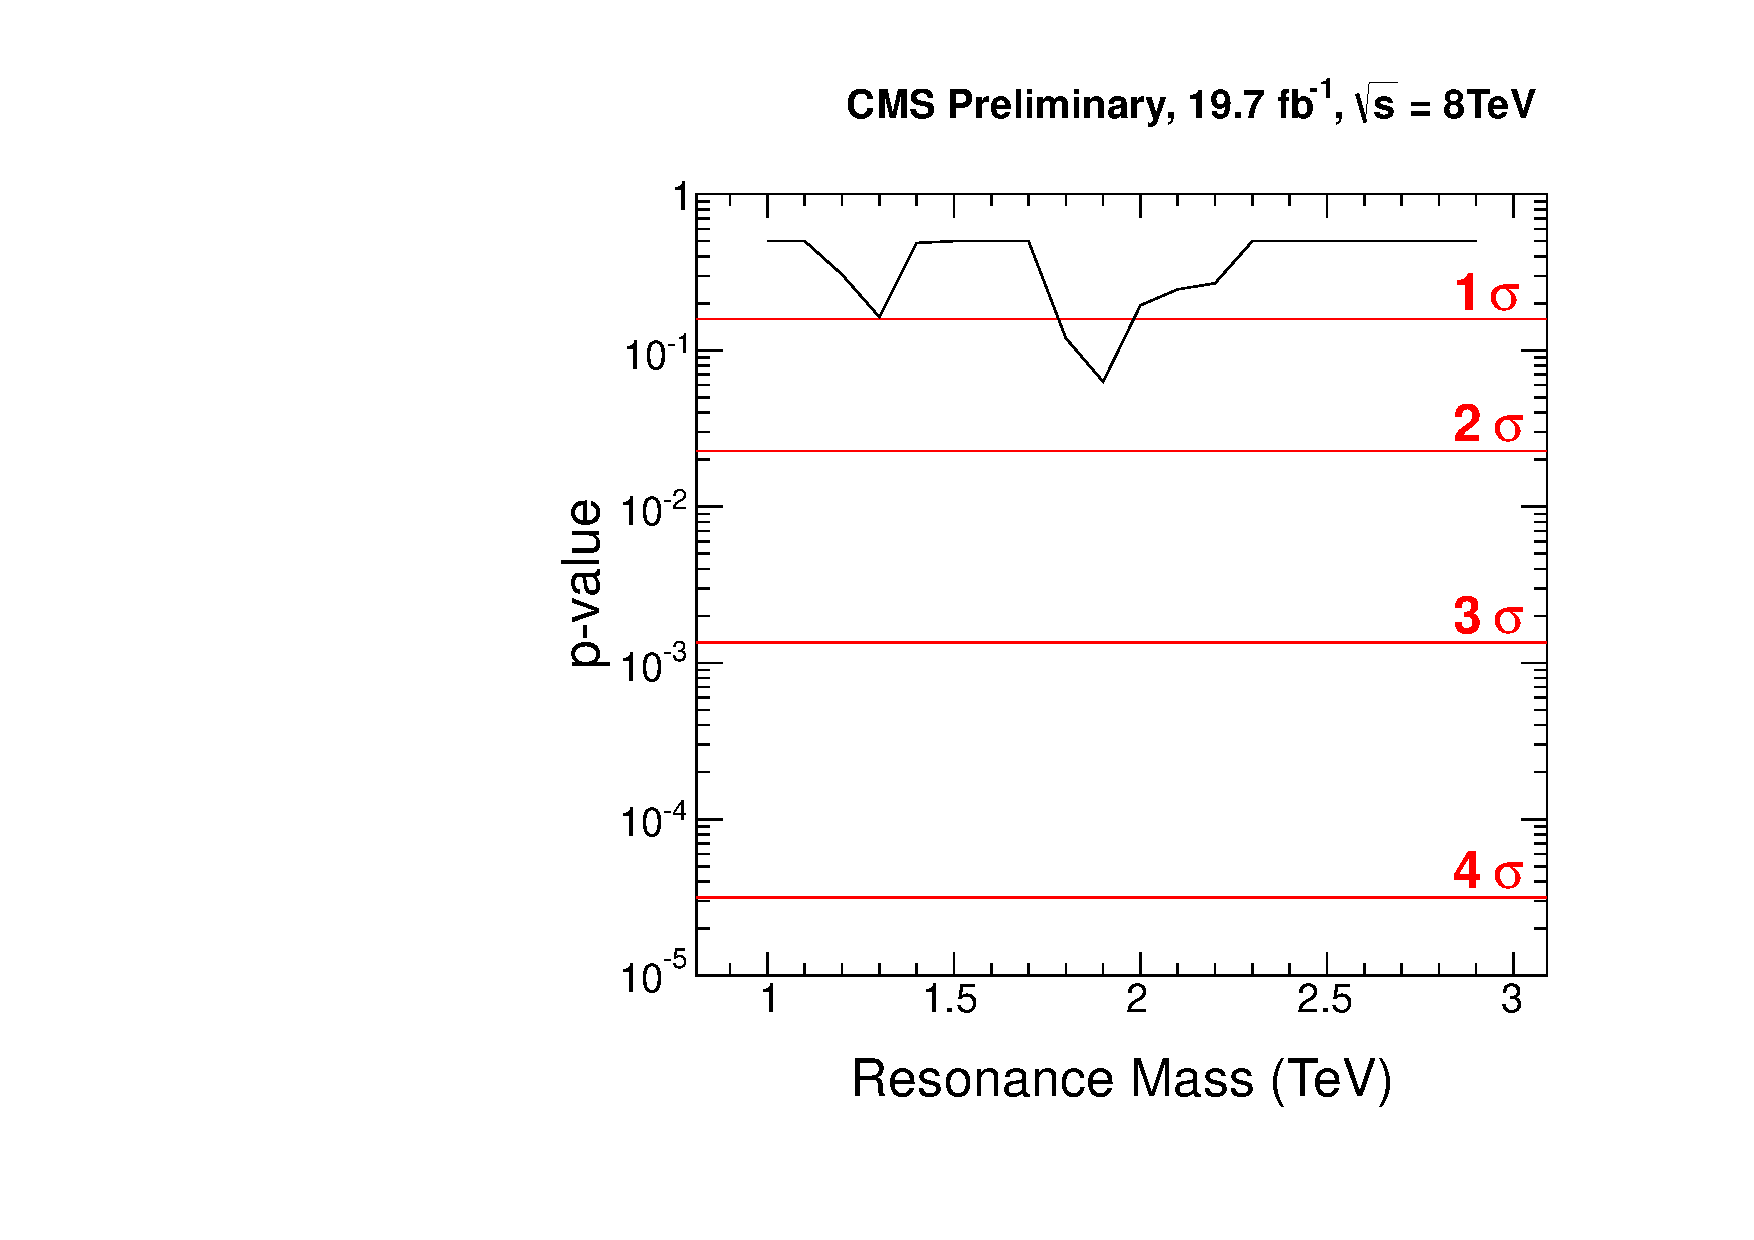
\includegraphics[width=0.35\textwidth]{figs/limits/pvalue_RS1WW_combined.pdf}
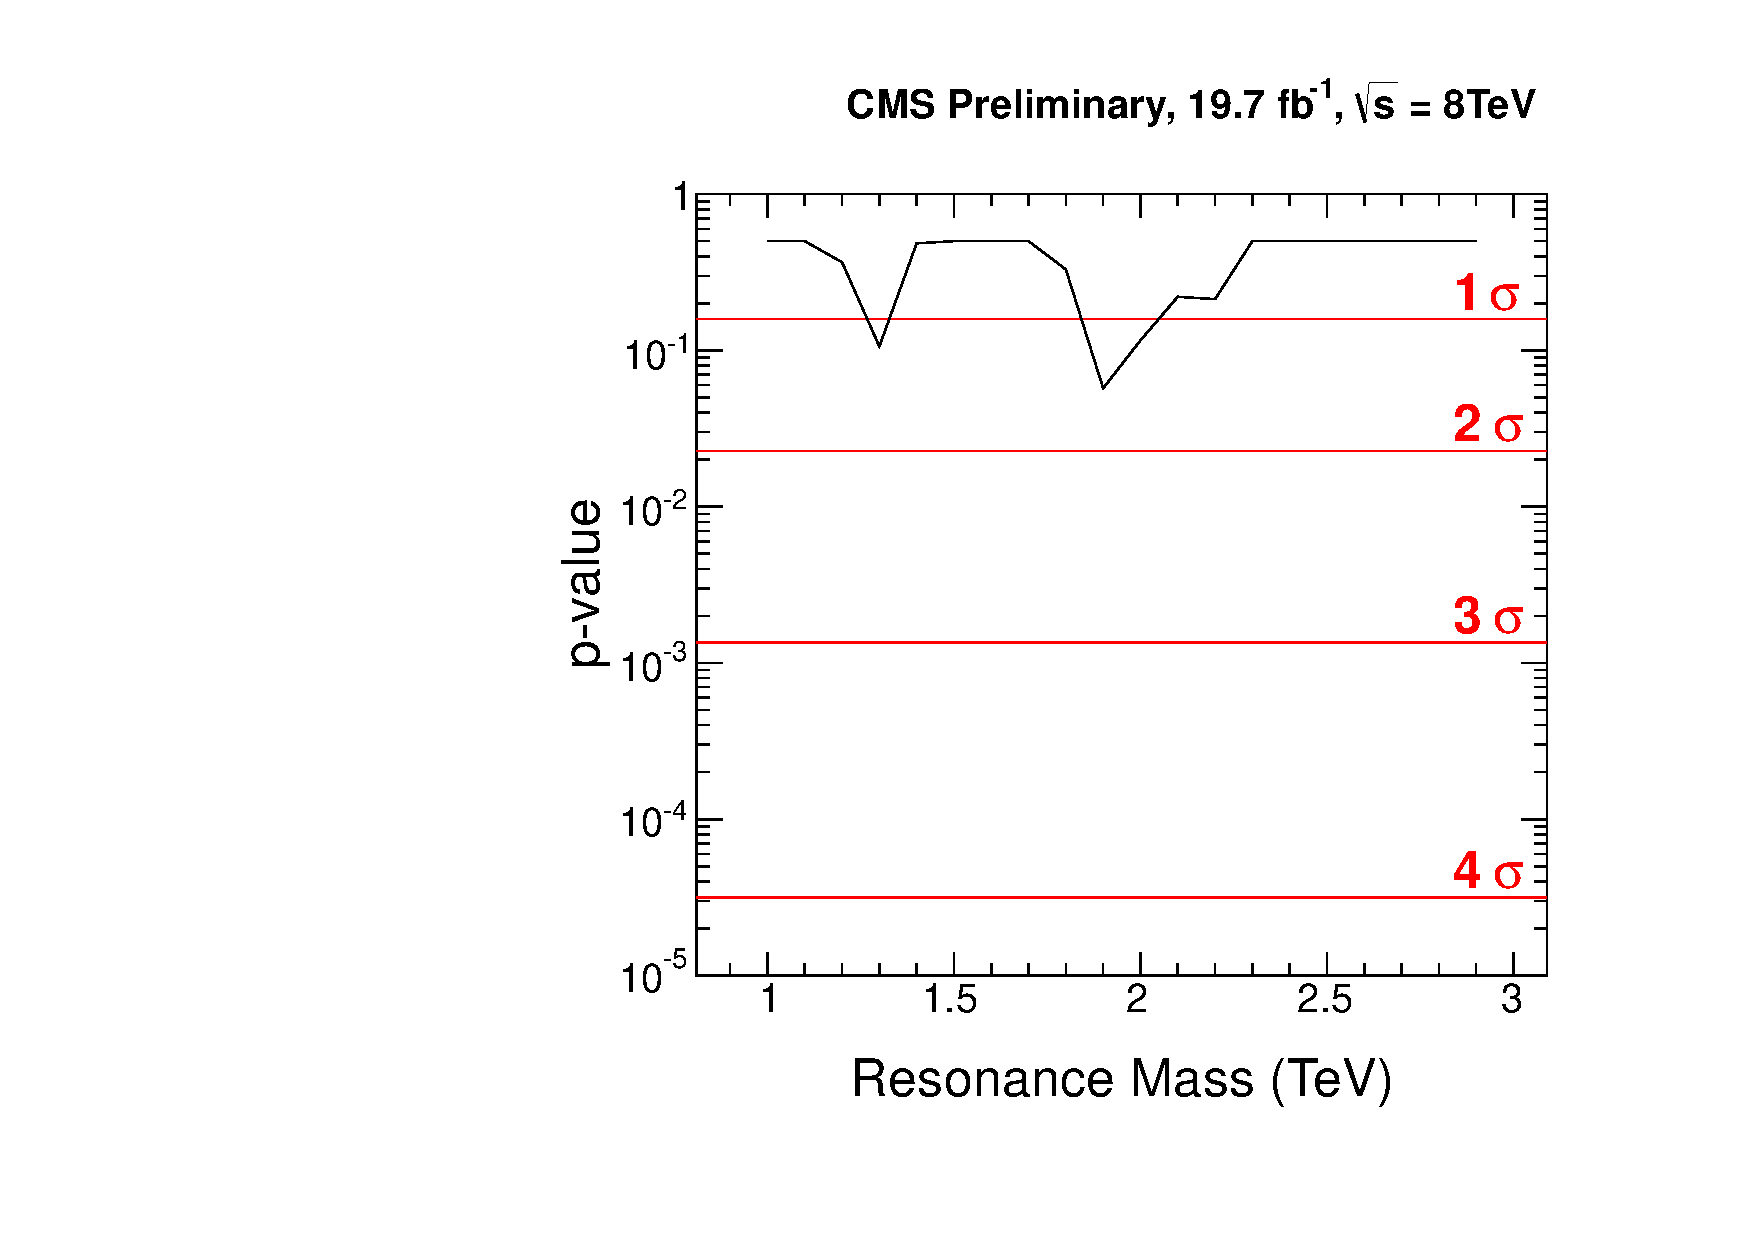
\includegraphics[width=0.35\textwidth]{figs/limits/pvalue_RS1ZZ_combined.pdf}
\end{center}
\caption{Observed local p-values assuming a \GRS WW (left) and \GRS ZZ (right) signal model in the doubly-tagged dijet mass spectrum in the low-purity (top), high-purity (middle) and combination (botton).}
\label{fig:Vtagresults5}
\end{figure*}

\begin{figure*}[h!tpb]
\begin{center}
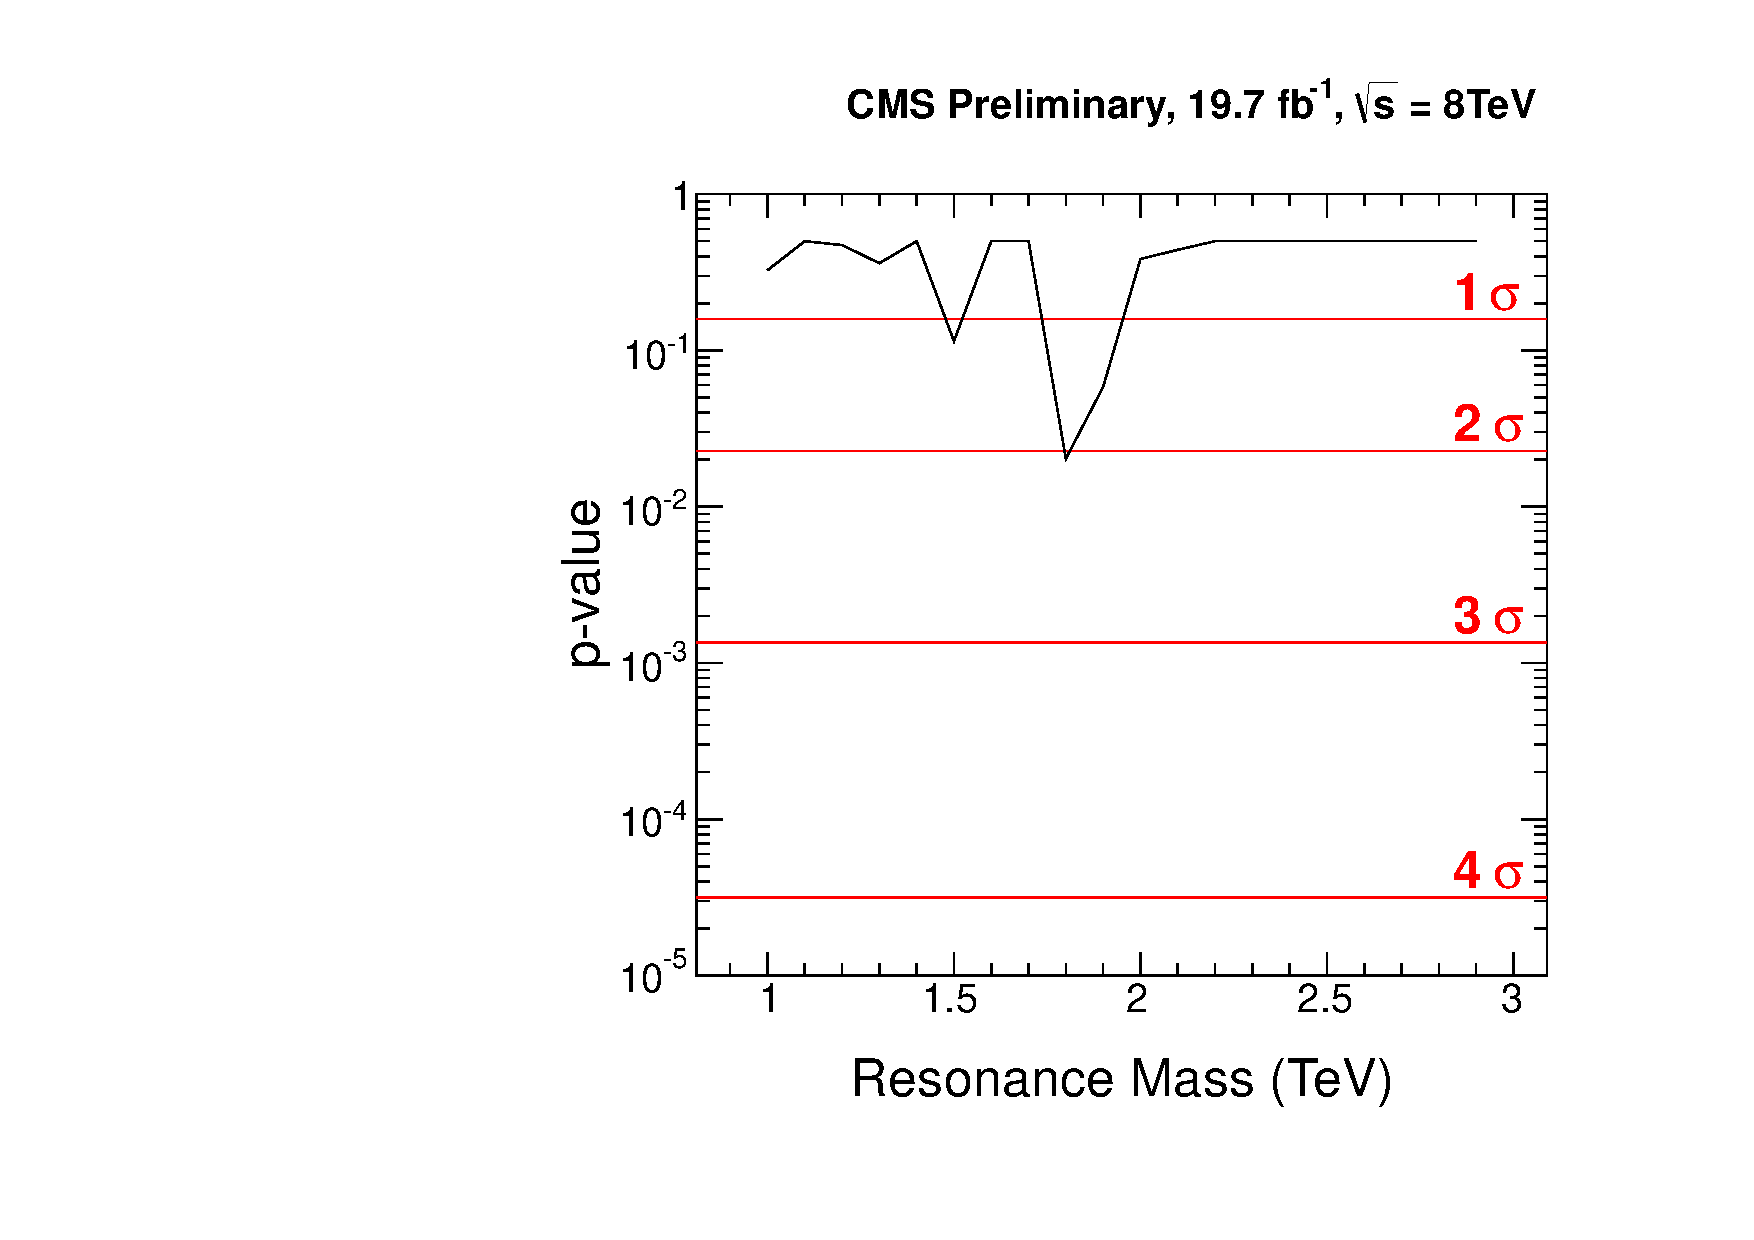
\includegraphics[width=0.35\textwidth]{figs/limits/pvalue_BulkWW_low_purity.pdf}
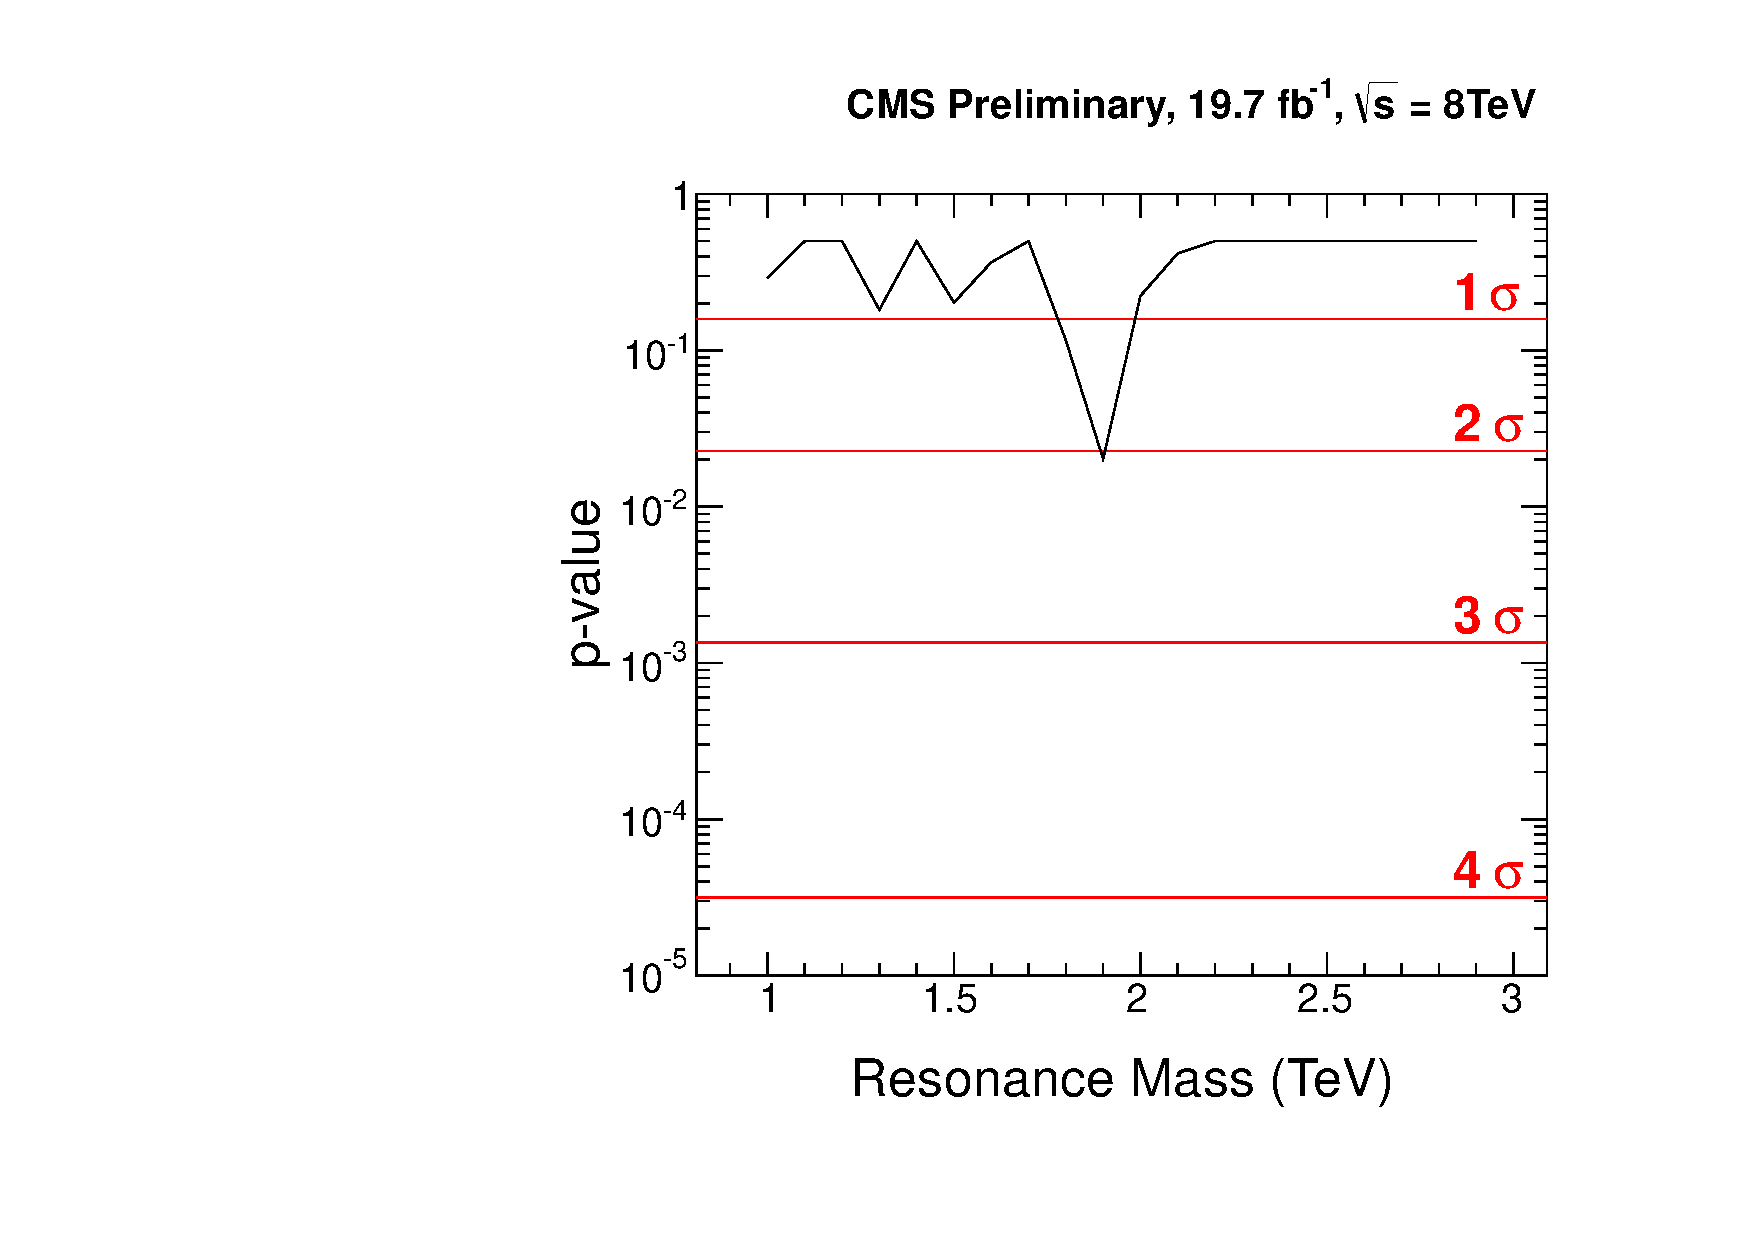
\includegraphics[width=0.35\textwidth]{figs/limits/pvalue_BulkZZ_low_purity.pdf}\\
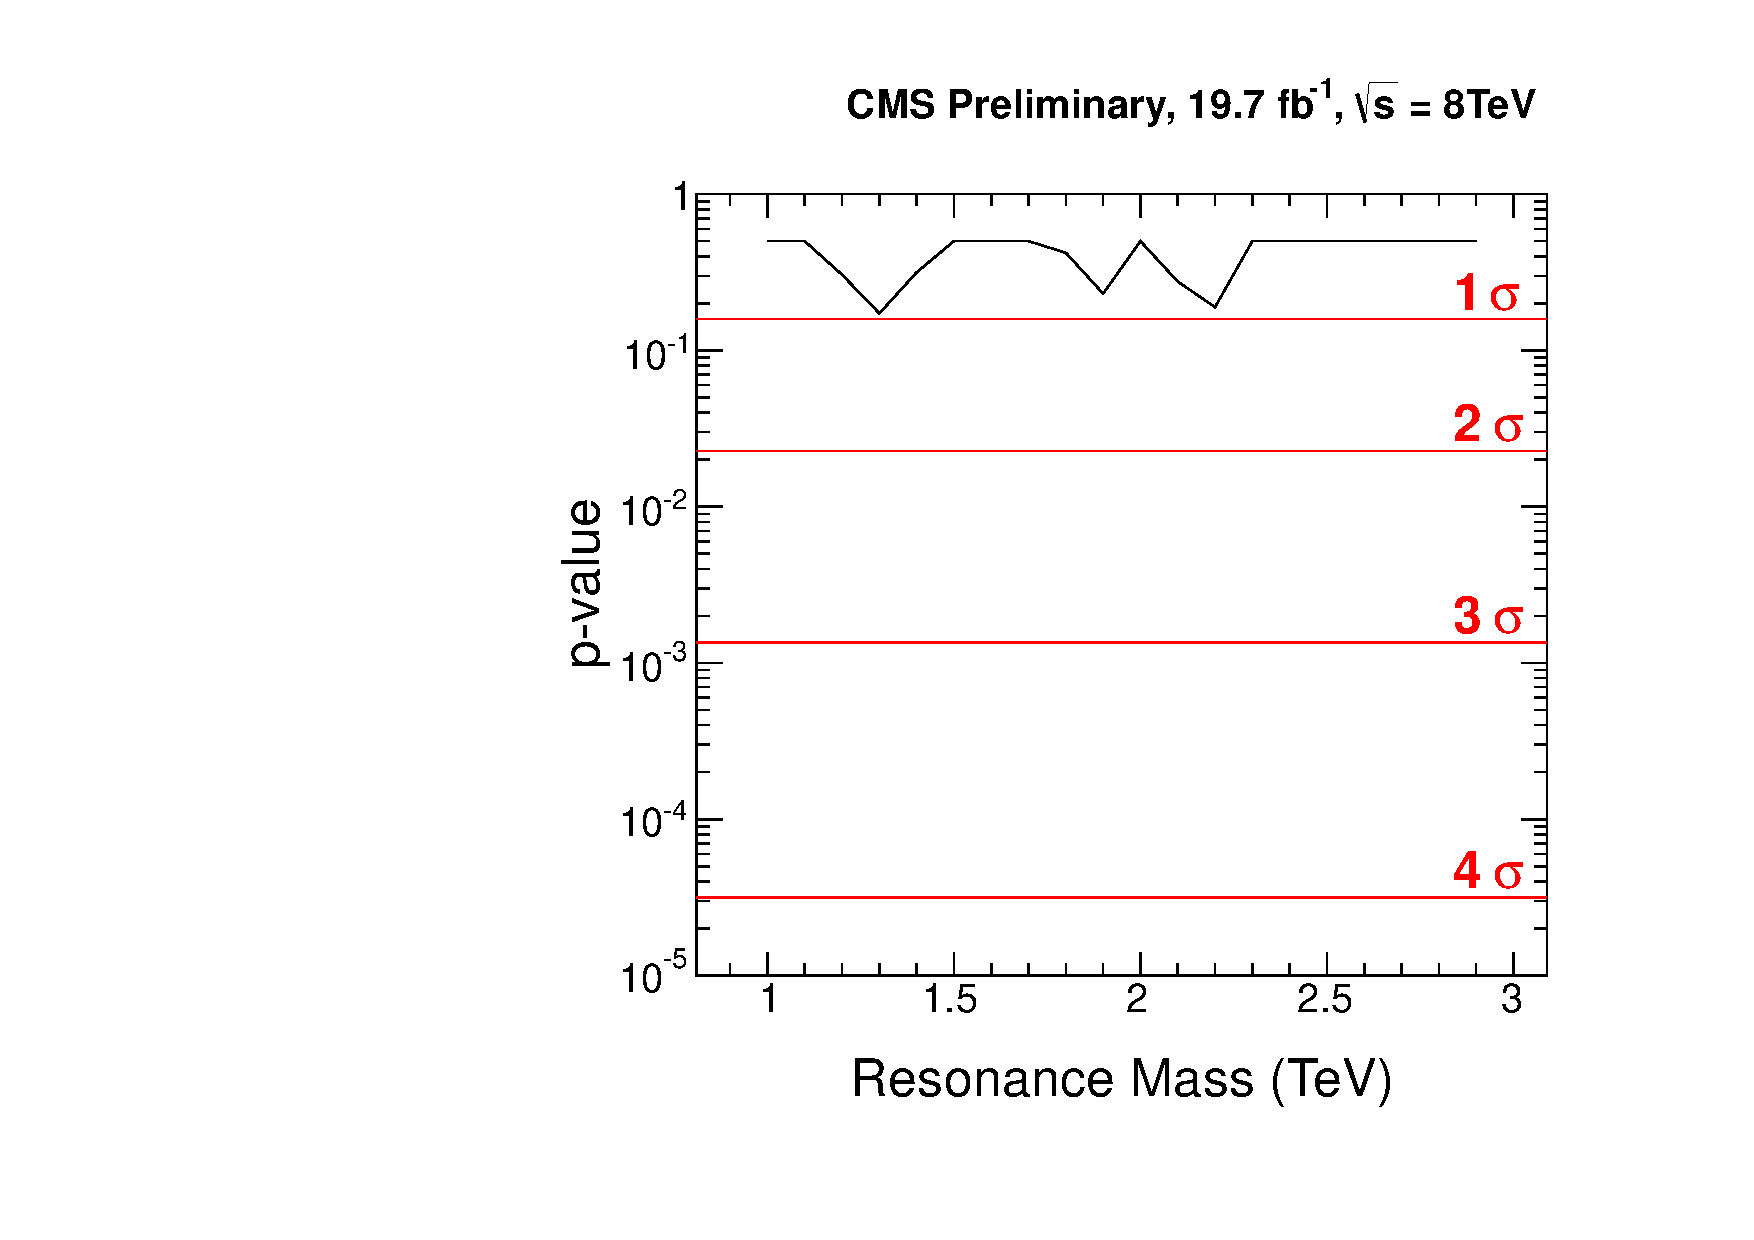
\includegraphics[width=0.35\textwidth]{figs/limits/pvalue_BulkWW_high_purity.pdf}
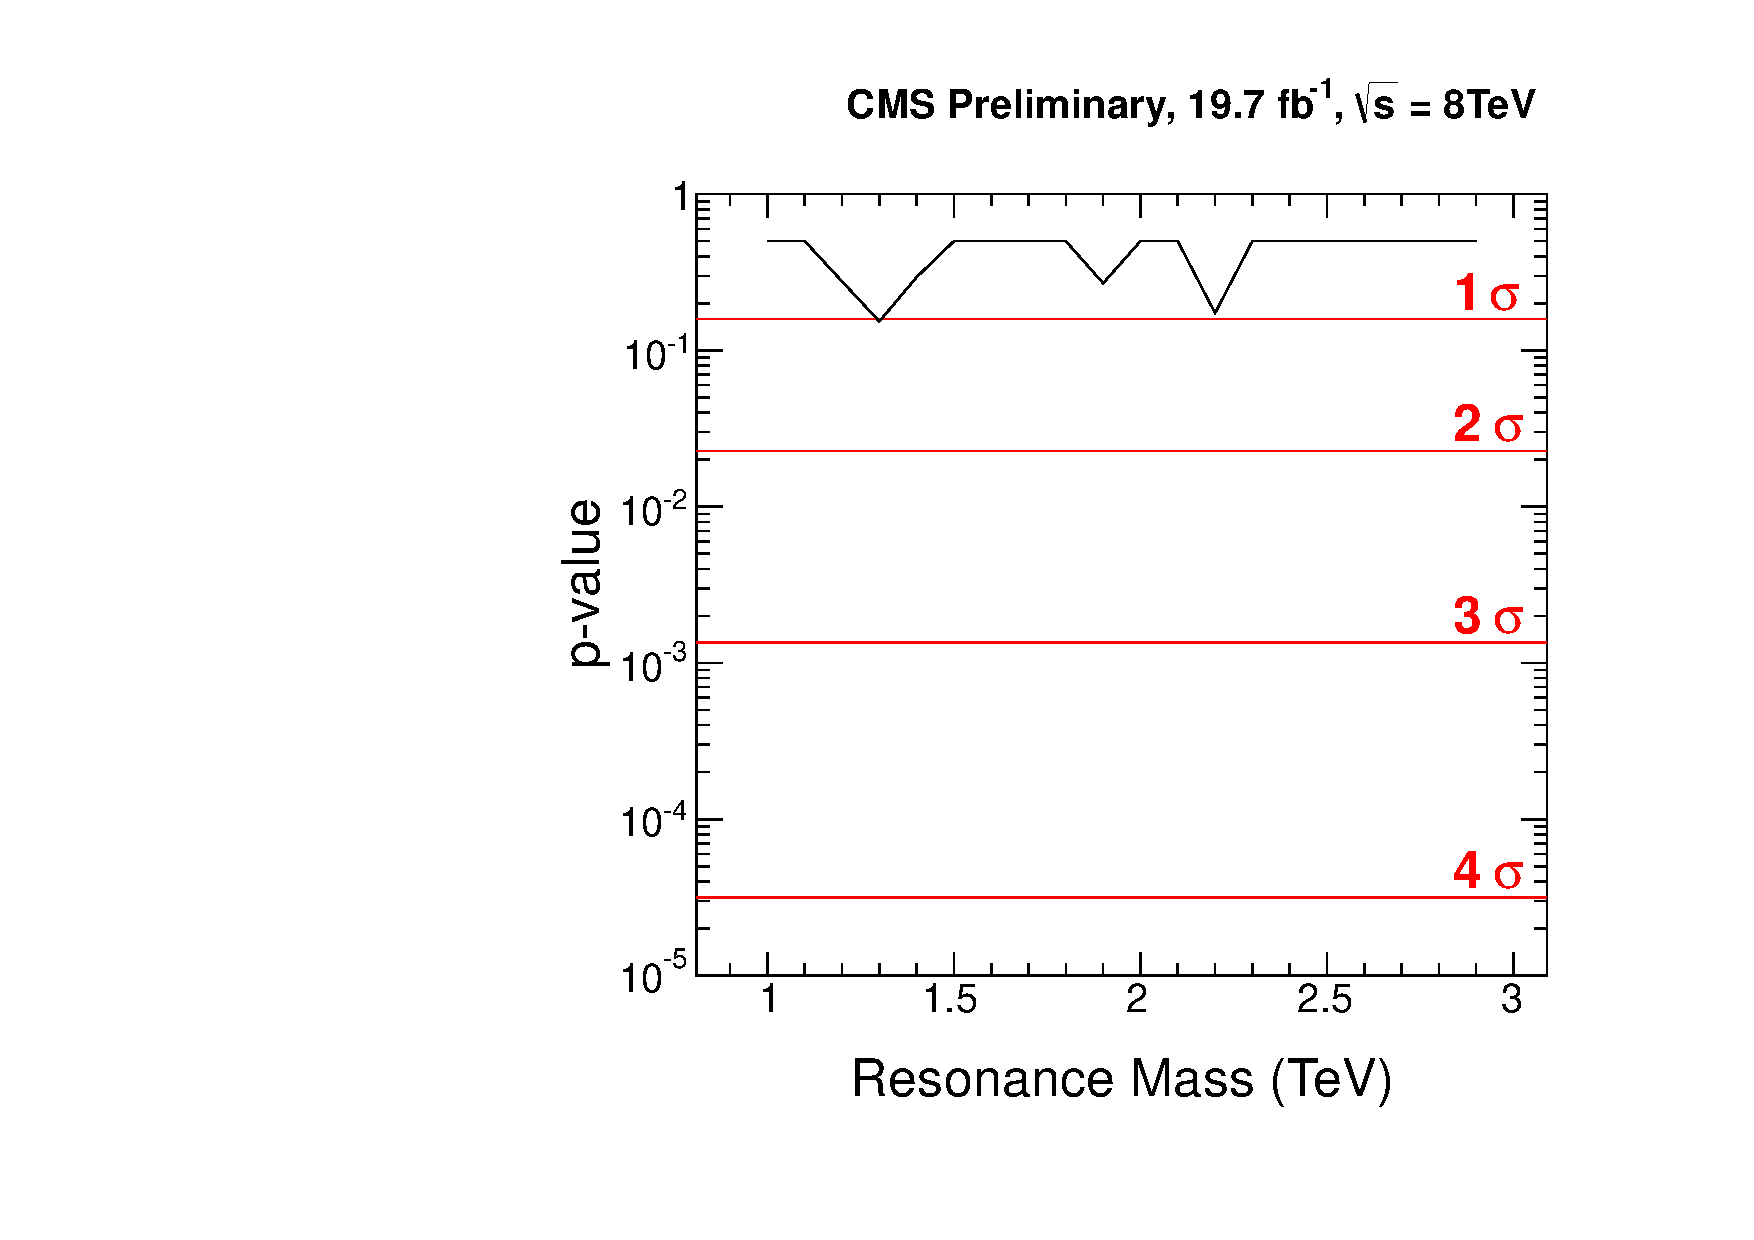
\includegraphics[width=0.35\textwidth]{figs/limits/pvalue_BulkZZ_high_purity.pdf}\\
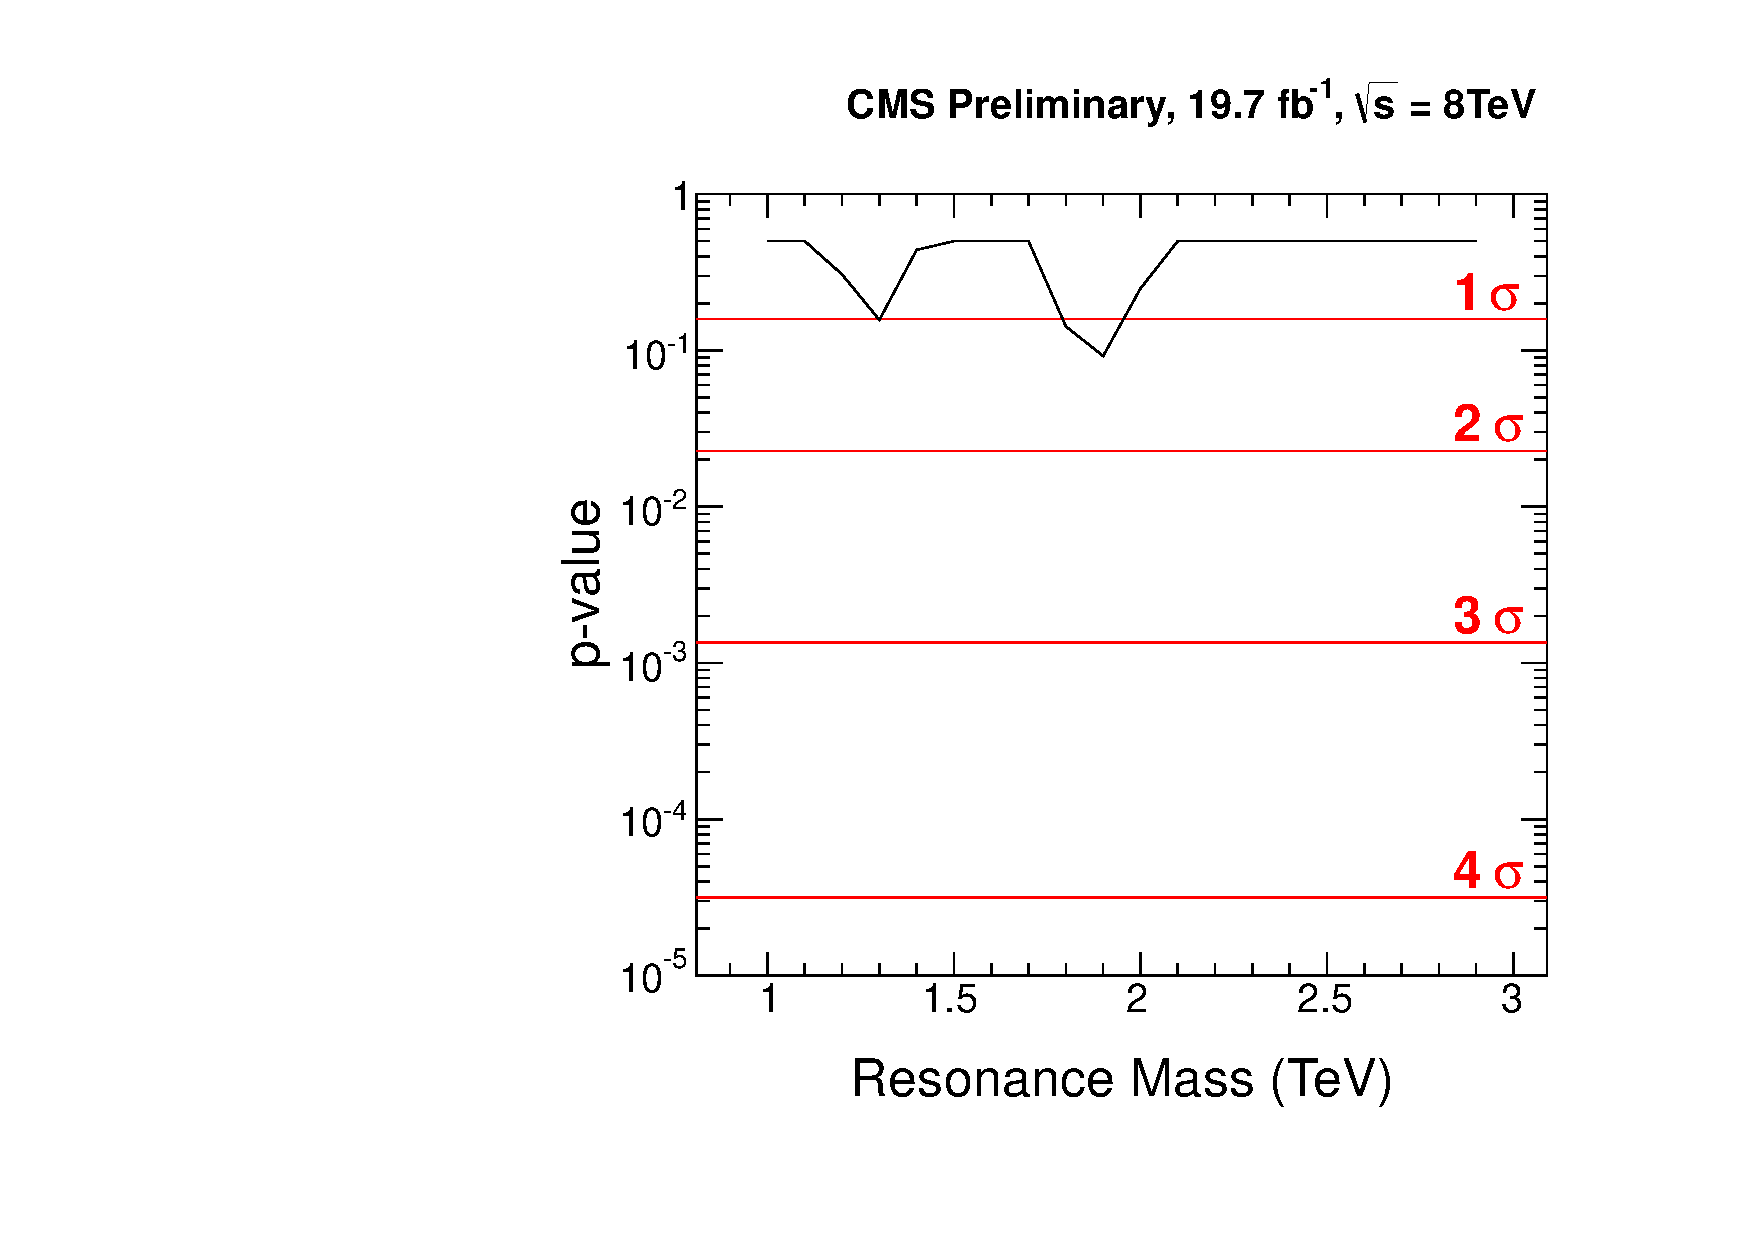
\includegraphics[width=0.35\textwidth]{figs/limits/pvalue_BulkWW_combined.pdf}
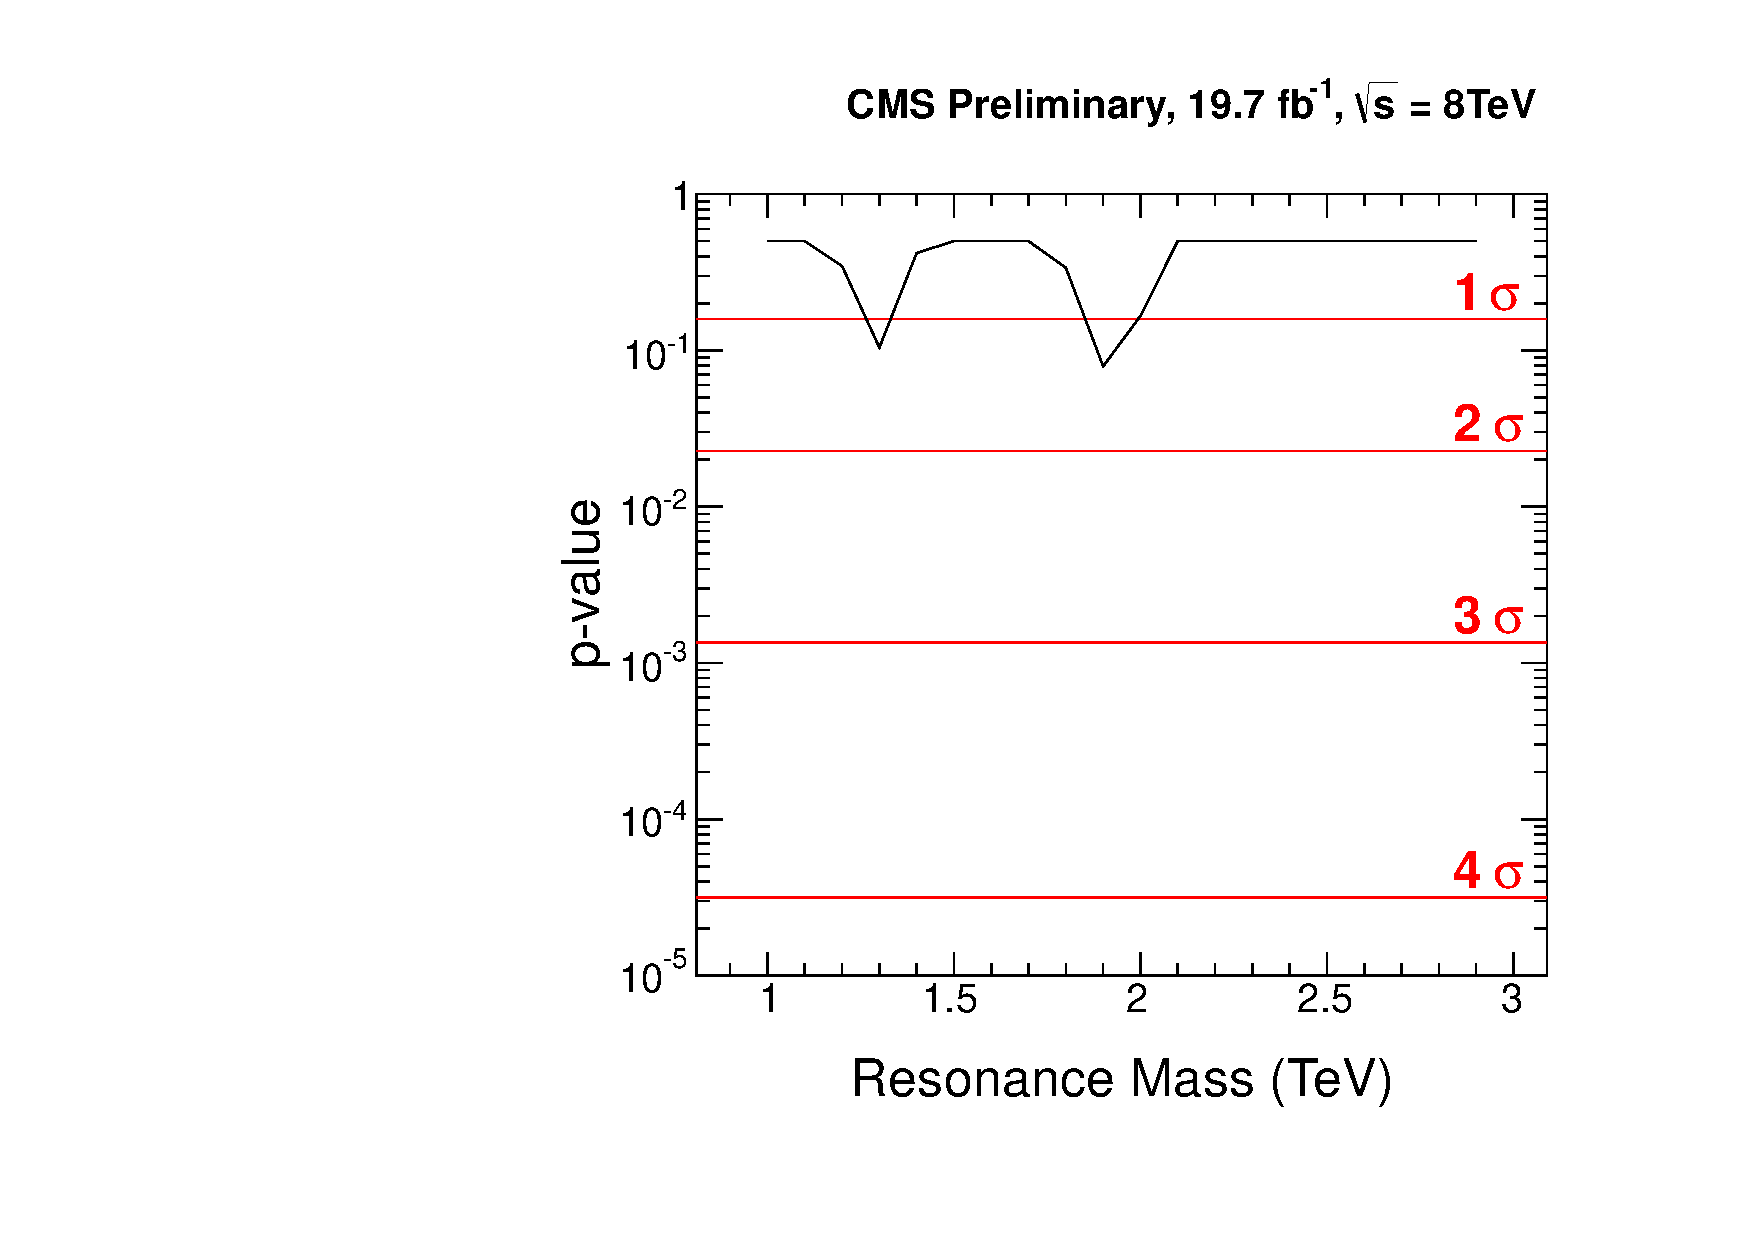
\includegraphics[width=0.35\textwidth]{figs/limits/pvalue_BulkZZ_combined.pdf}
\end{center}
\caption{Observed local p-values assuming a \GBulk WW (left) and \GBulk ZZ (right) signal model in the doubly-tagged dijet mass spectrum in the low-purity (top), high-purity (middle) and combination (botton).}
\label{fig:Vtagresults52}
\end{figure*}

\begin{figure*}[h!tpb]
\begin{center}
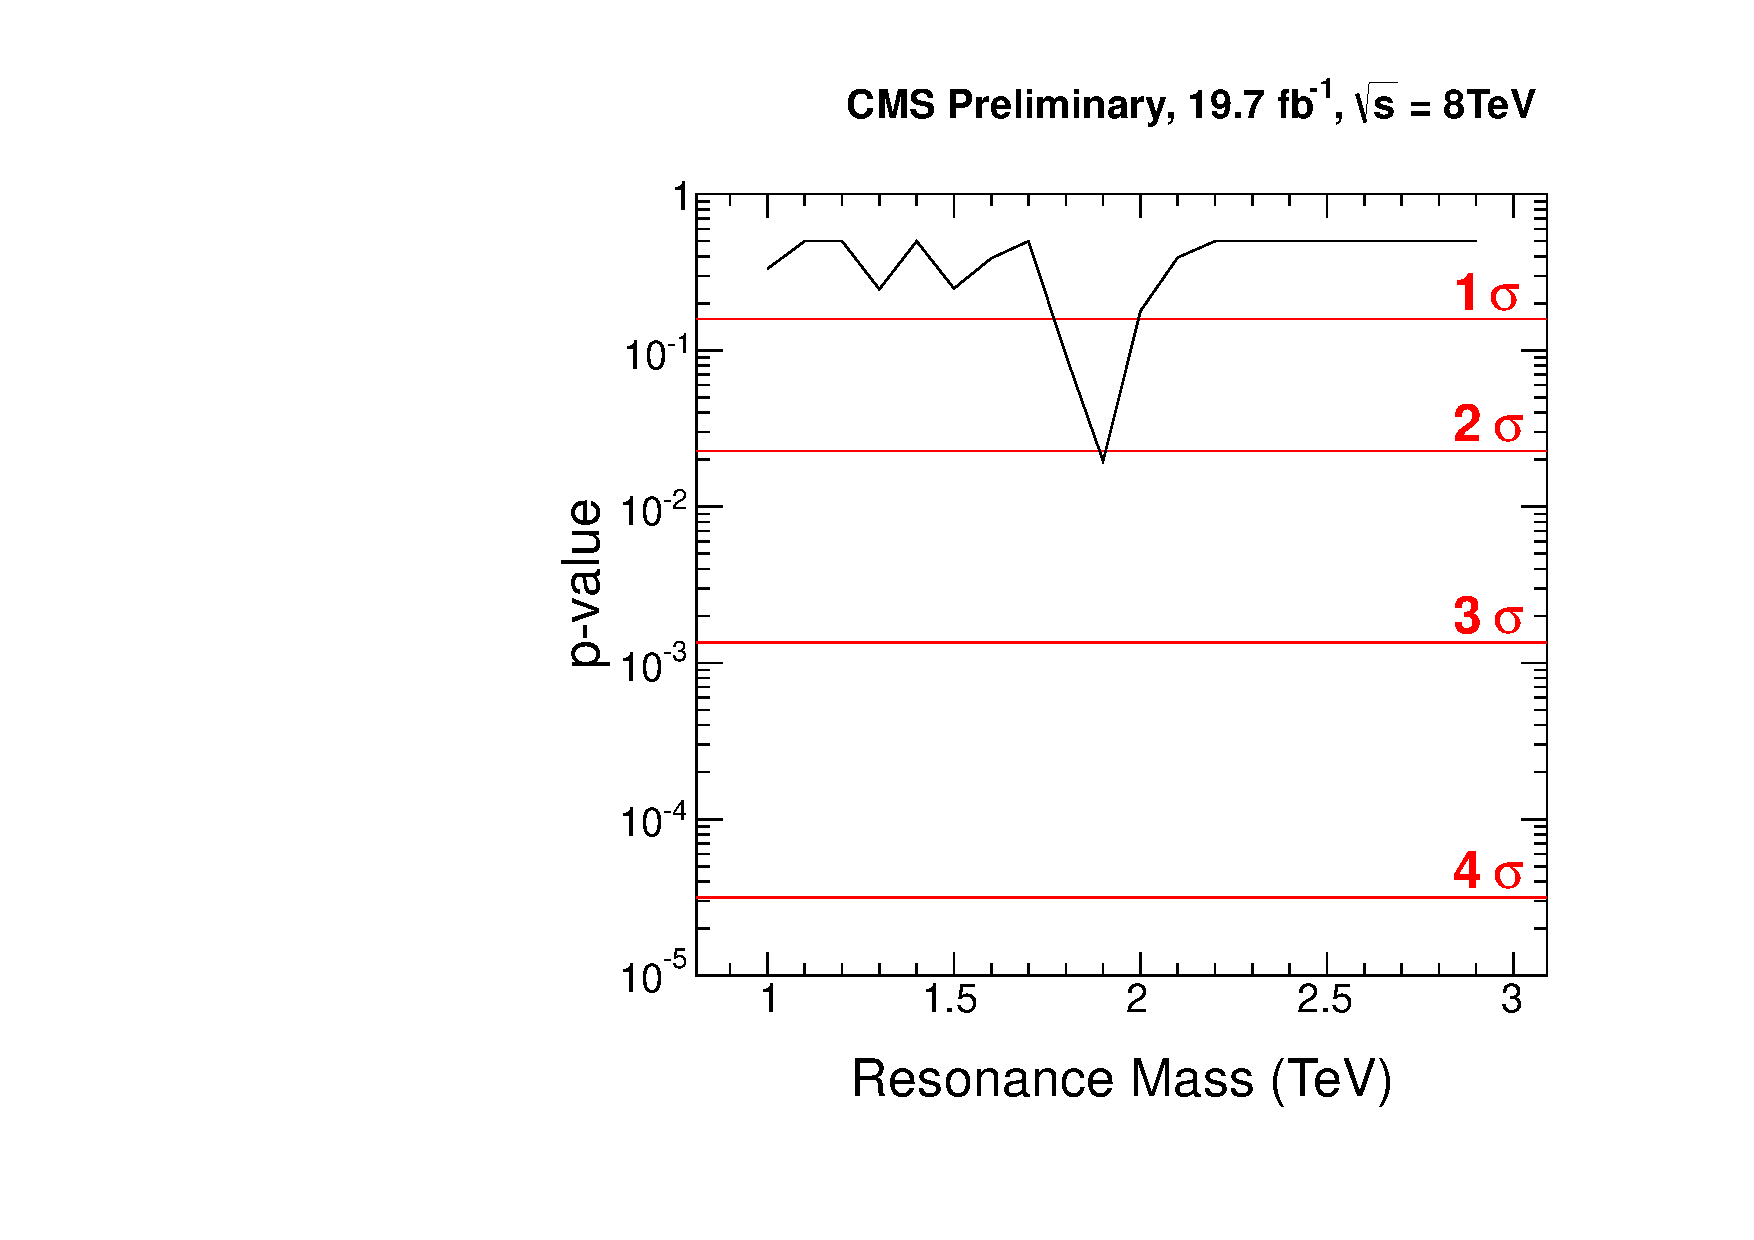
\includegraphics[width=0.35\textwidth]{figs/limits/pvalue_WZ_low_purity.pdf}\\
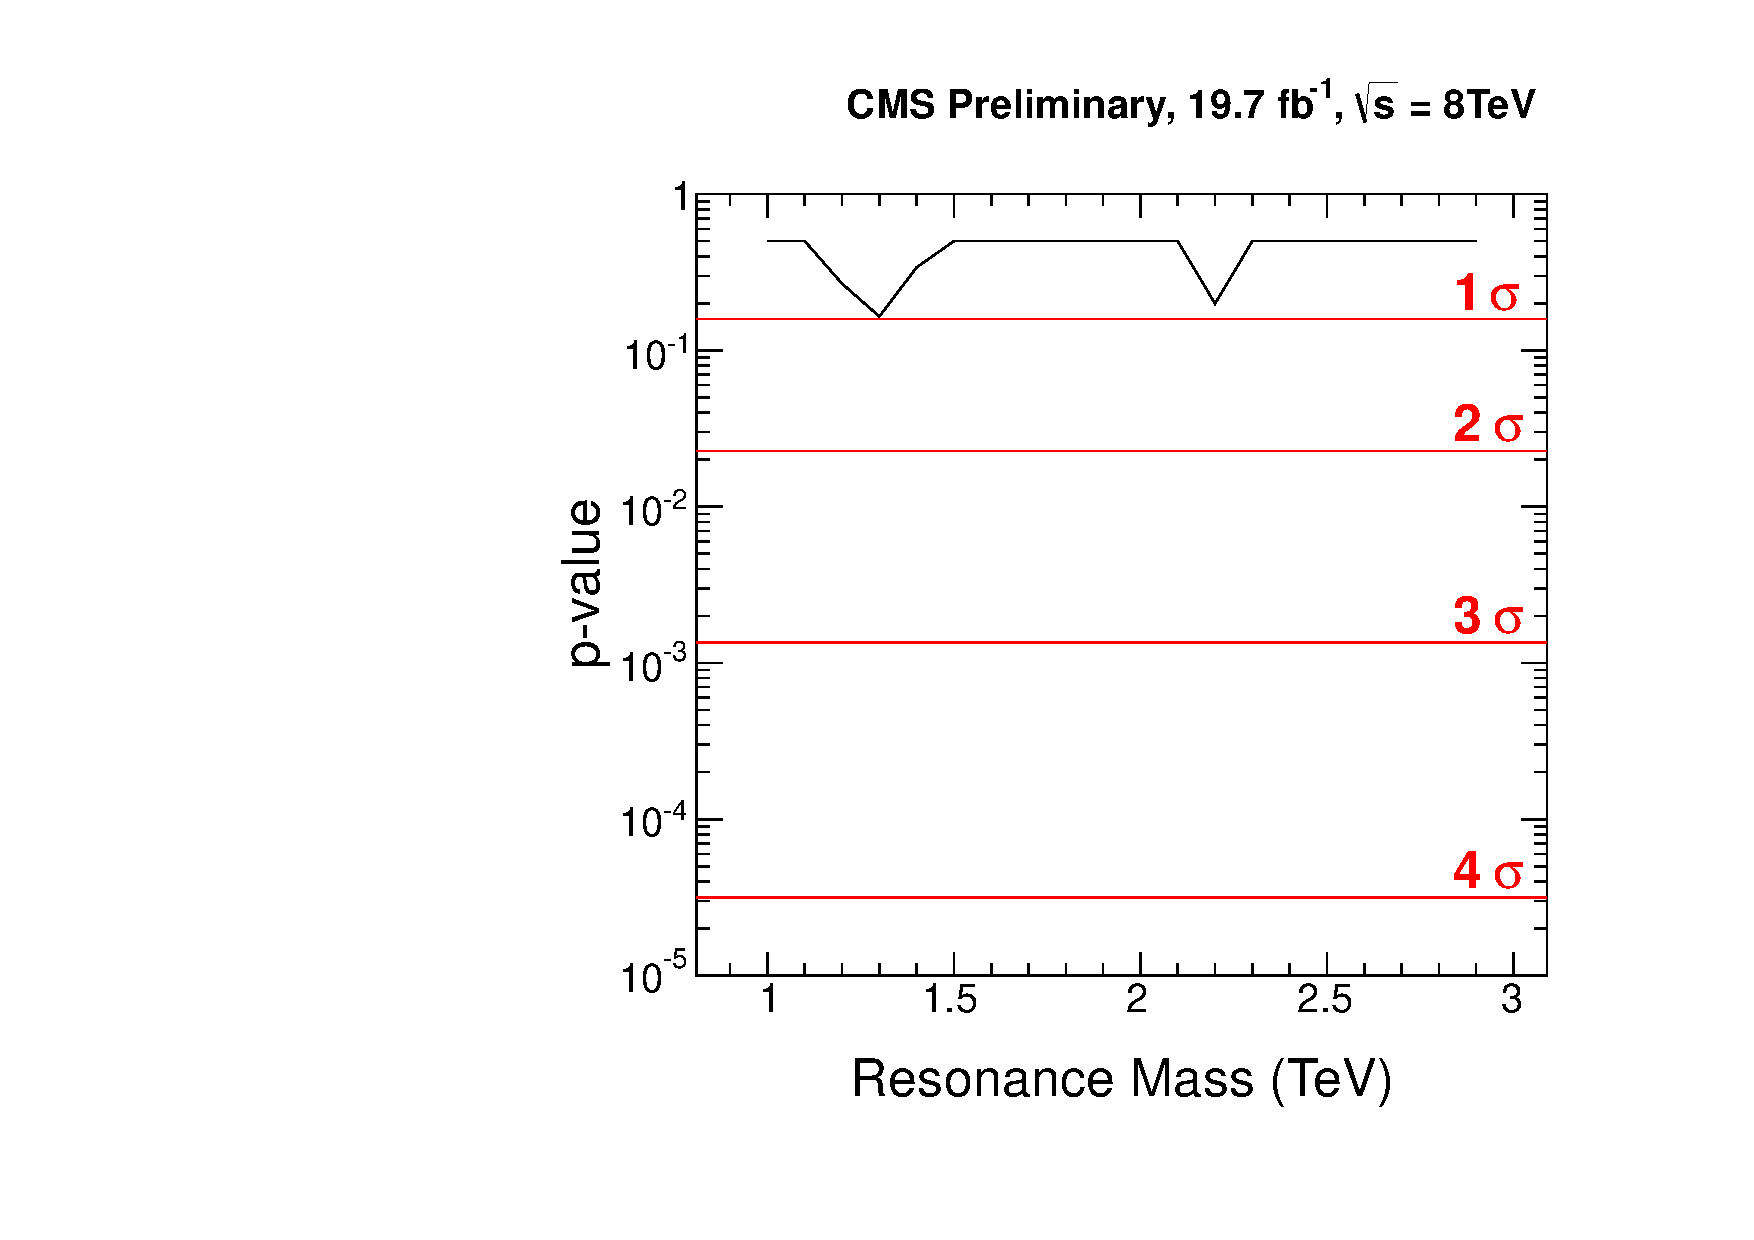
\includegraphics[width=0.35\textwidth]{figs/limits/pvalue_WZ_high_purity.pdf}\\
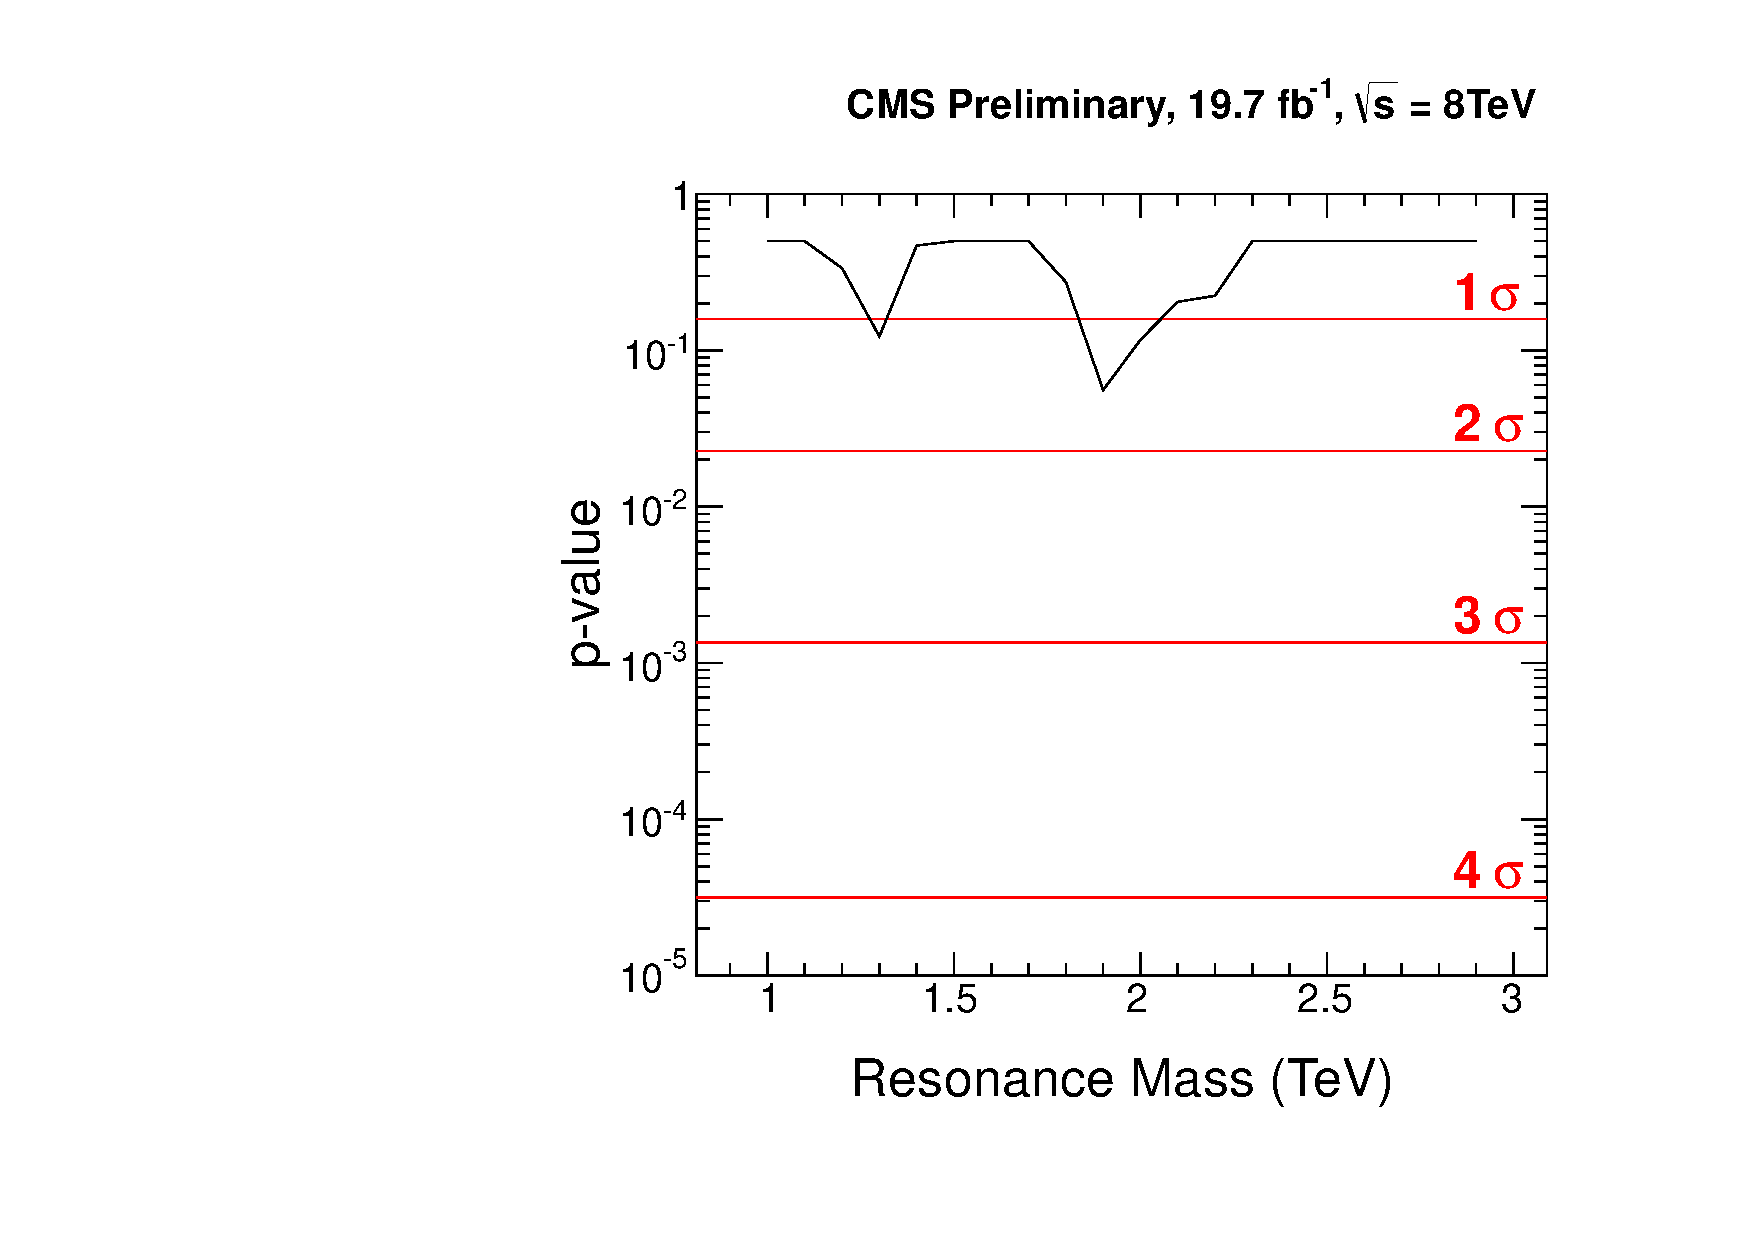
\includegraphics[width=0.35\textwidth]{figs/limits/pvalue_WZ_combined.pdf}
\end{center}
\caption{Observed local p-values assuming a WZ signal model in the doubly-tagged dijet mass spectrum in the low-purity (top), high-purity (middle) and combination (botton).}
\label{fig:Vtagresults6}
\end{figure*}

\begin{figure}[htb]
\begin{center}
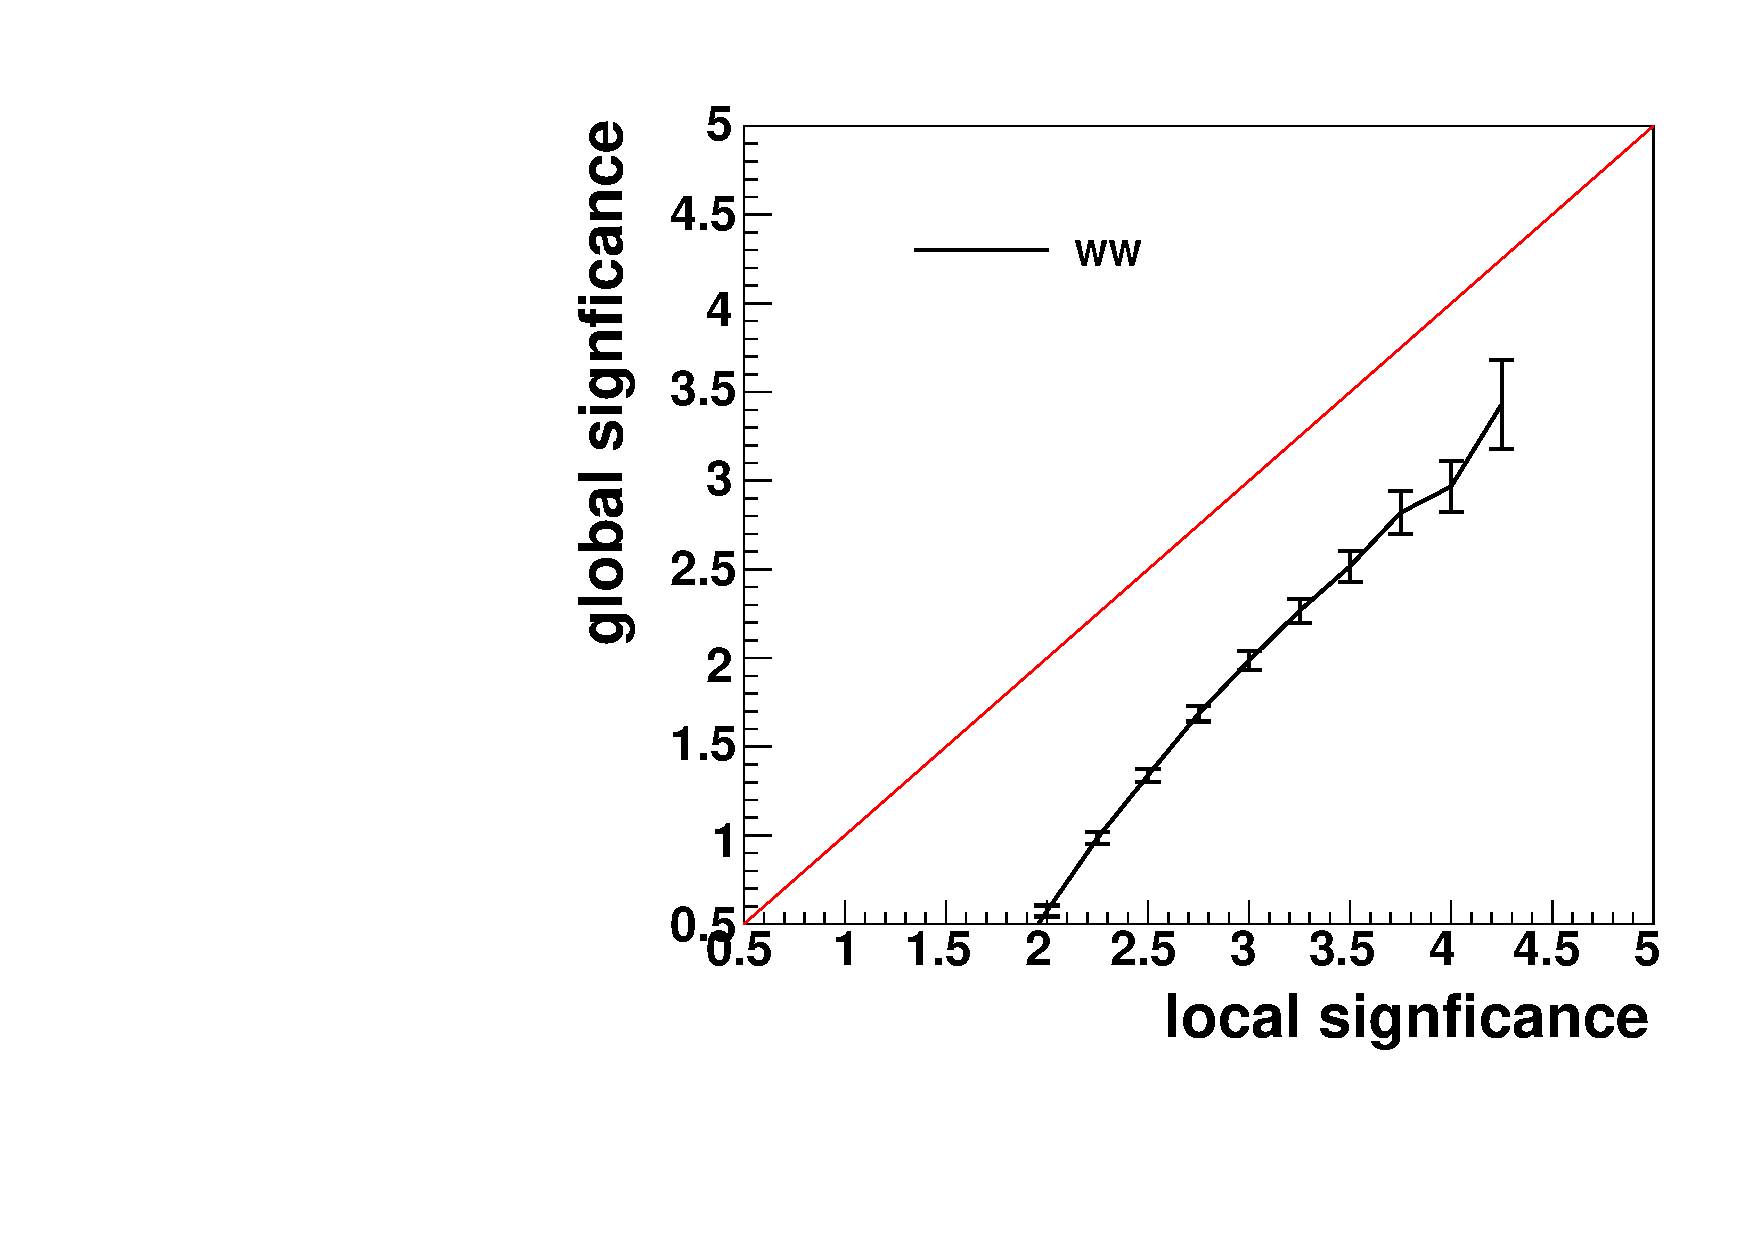
\includegraphics[width=0.48\textwidth,angle=0]{figs/appendix/Xvv_WW_8TeV_Sig_channel2_toys_1000_2300.pdf}
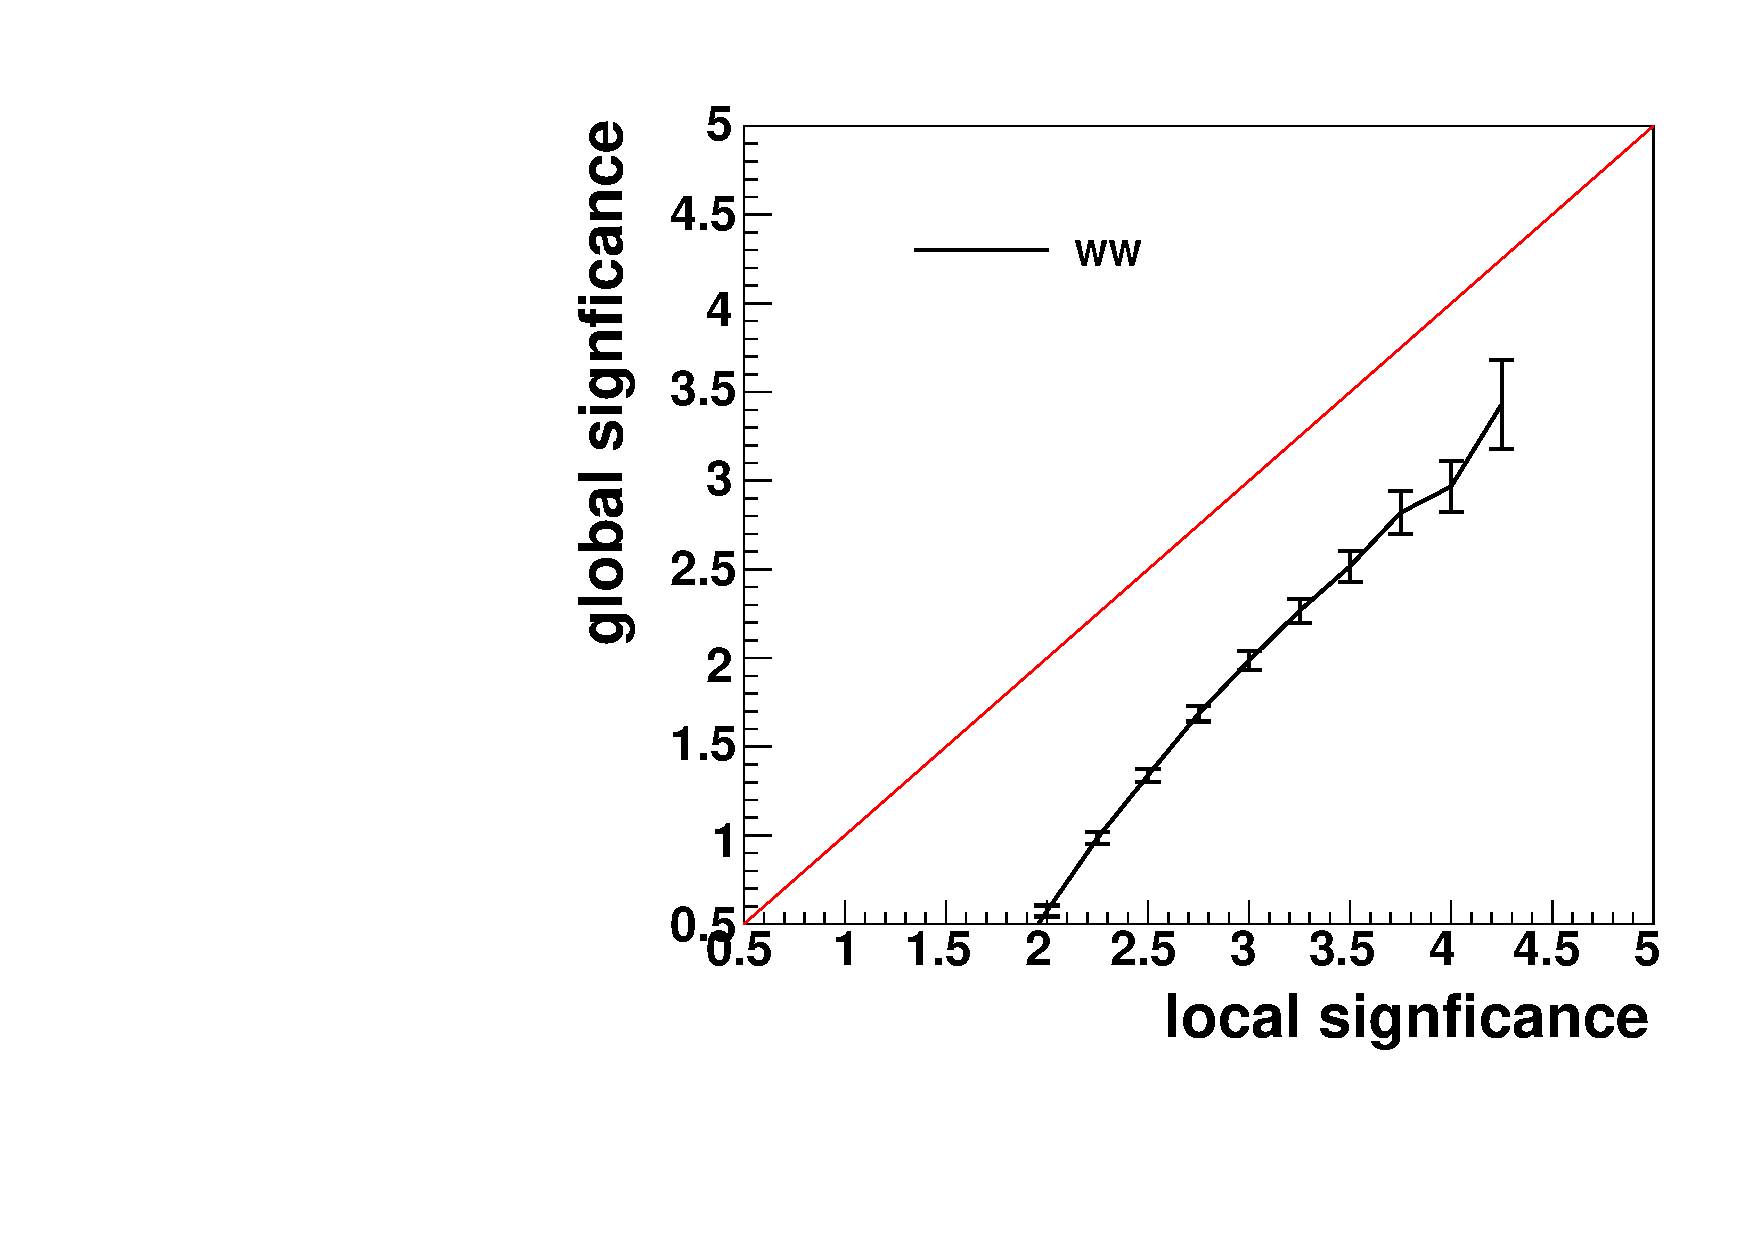
\includegraphics[width=0.48\textwidth,angle=0]{figs/appendix/Xvv_WW_8TeV_Sig_channel2_toys_1200_2300.pdf}
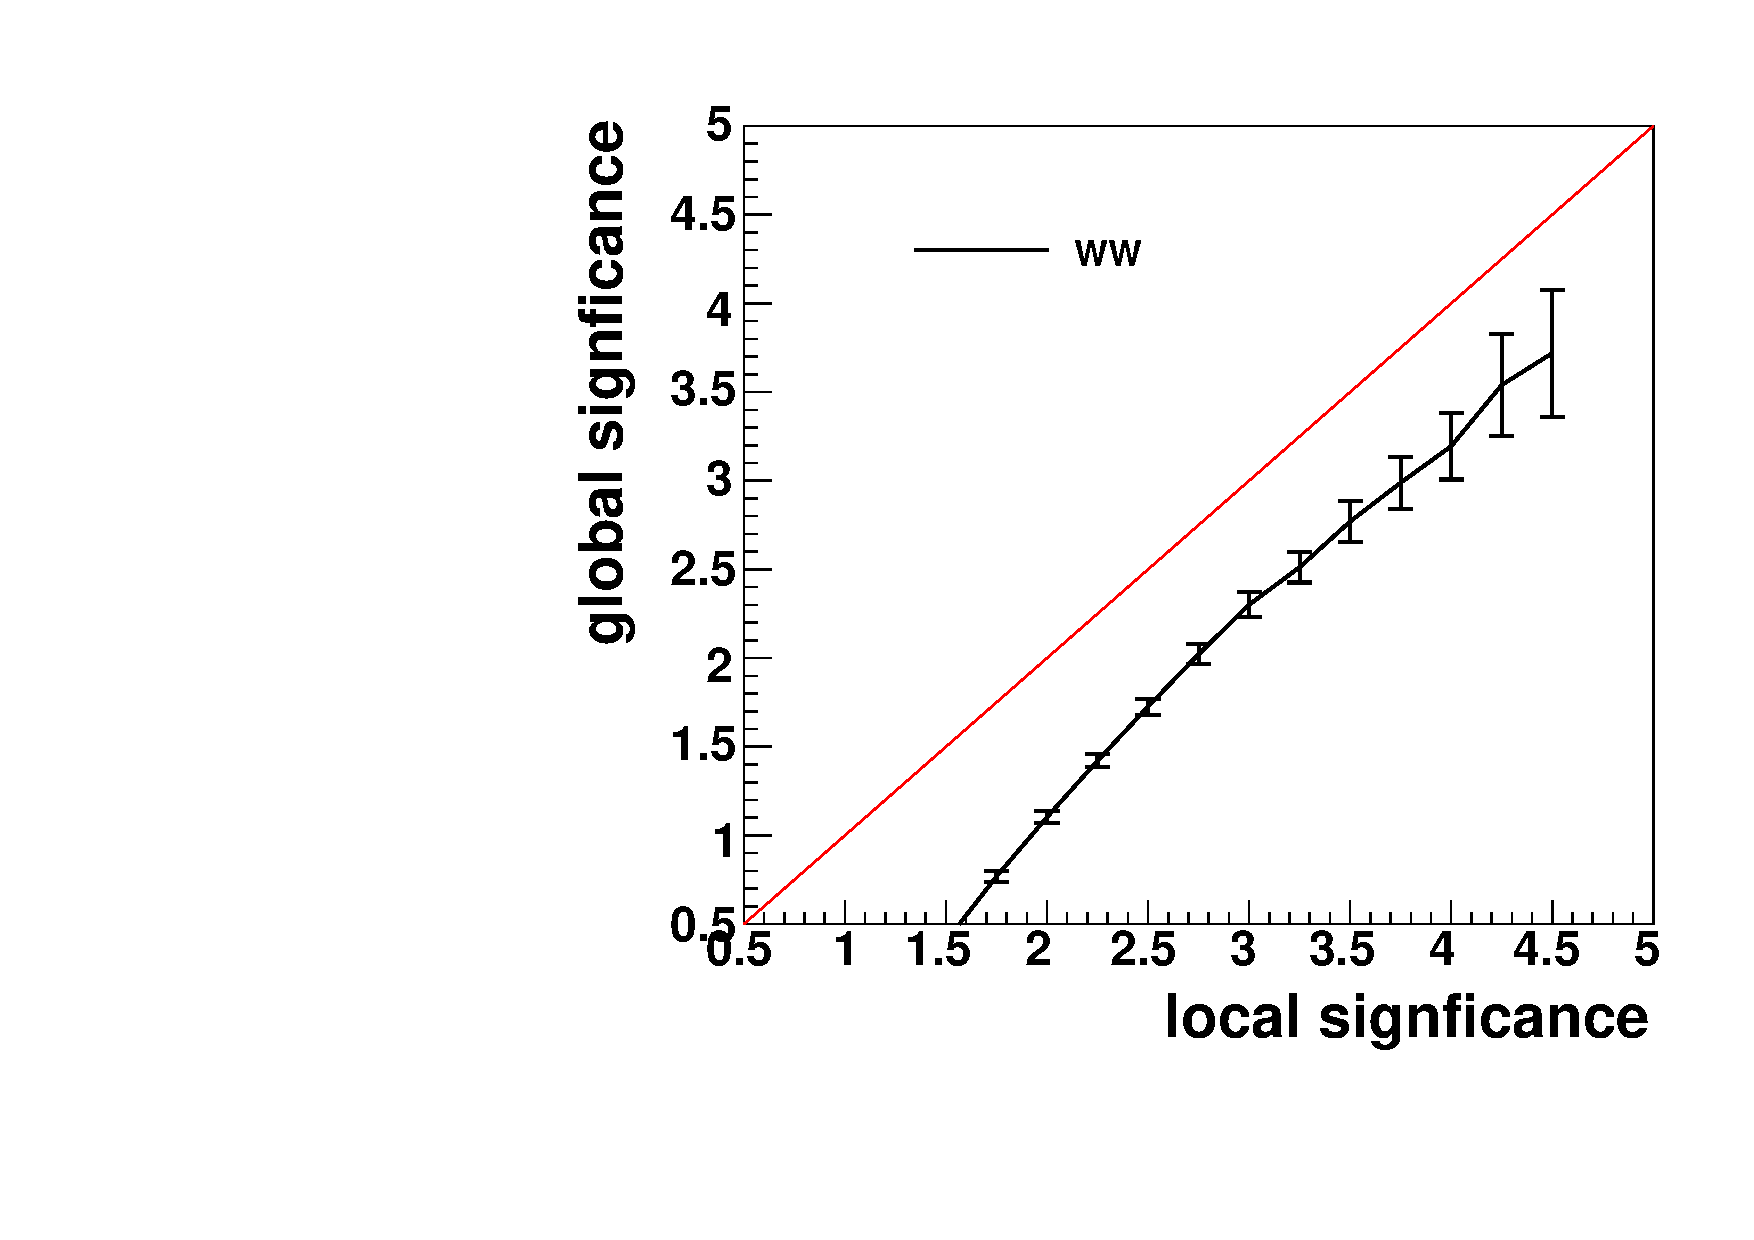
\includegraphics[width=0.48\textwidth,angle=0]{figs/appendix/Xvv_WW_8TeV_Sig_channel2_toys_1500_2000.pdf}
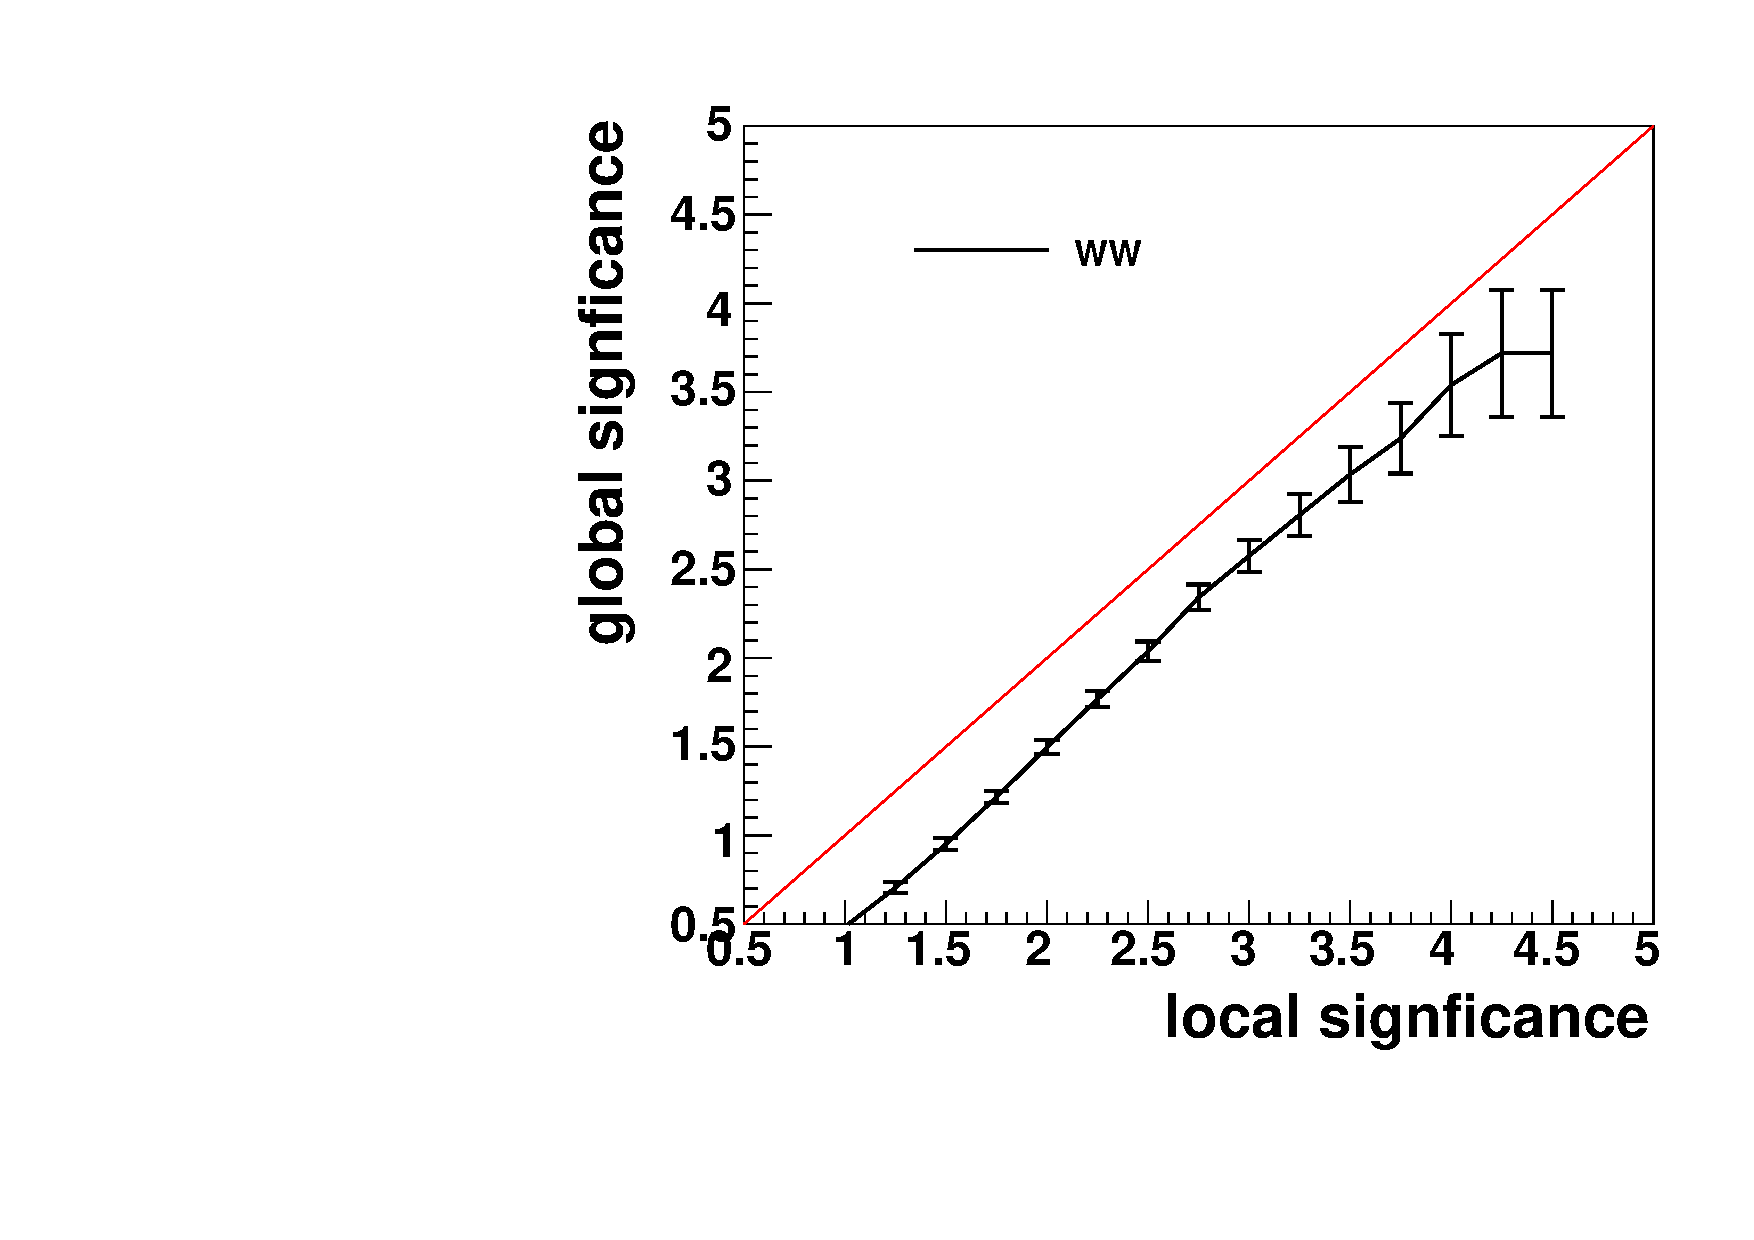
\includegraphics[width=0.48\textwidth,angle=0]{figs/appendix/Xvv_WW_8TeV_Sig_channel2_toys_2000_2300.pdf}
\end{center}
\caption{Estimate of the look-else-where effect for this search.
Shown is the global significance as a function
of the local significance which corresponds to the maximal significance in the dijet mass distribution in the
mass ranges 1.0-2.3~TeV (top-left), 1.2-2.3~TeV (top-right), 1.5-2.0~TeV (bottom-left) and 2.0-2.3~TeV (bottom-right).
The global significance is estimated using background-only toys and corresponds to the fraction of toys
(translated from a p-value to significance) with at least a certain local signficance in the dijet mass distribution.}
\label{fig:lee}
\end{figure}

%\begin{figure}[htb]
%\begin{center}
%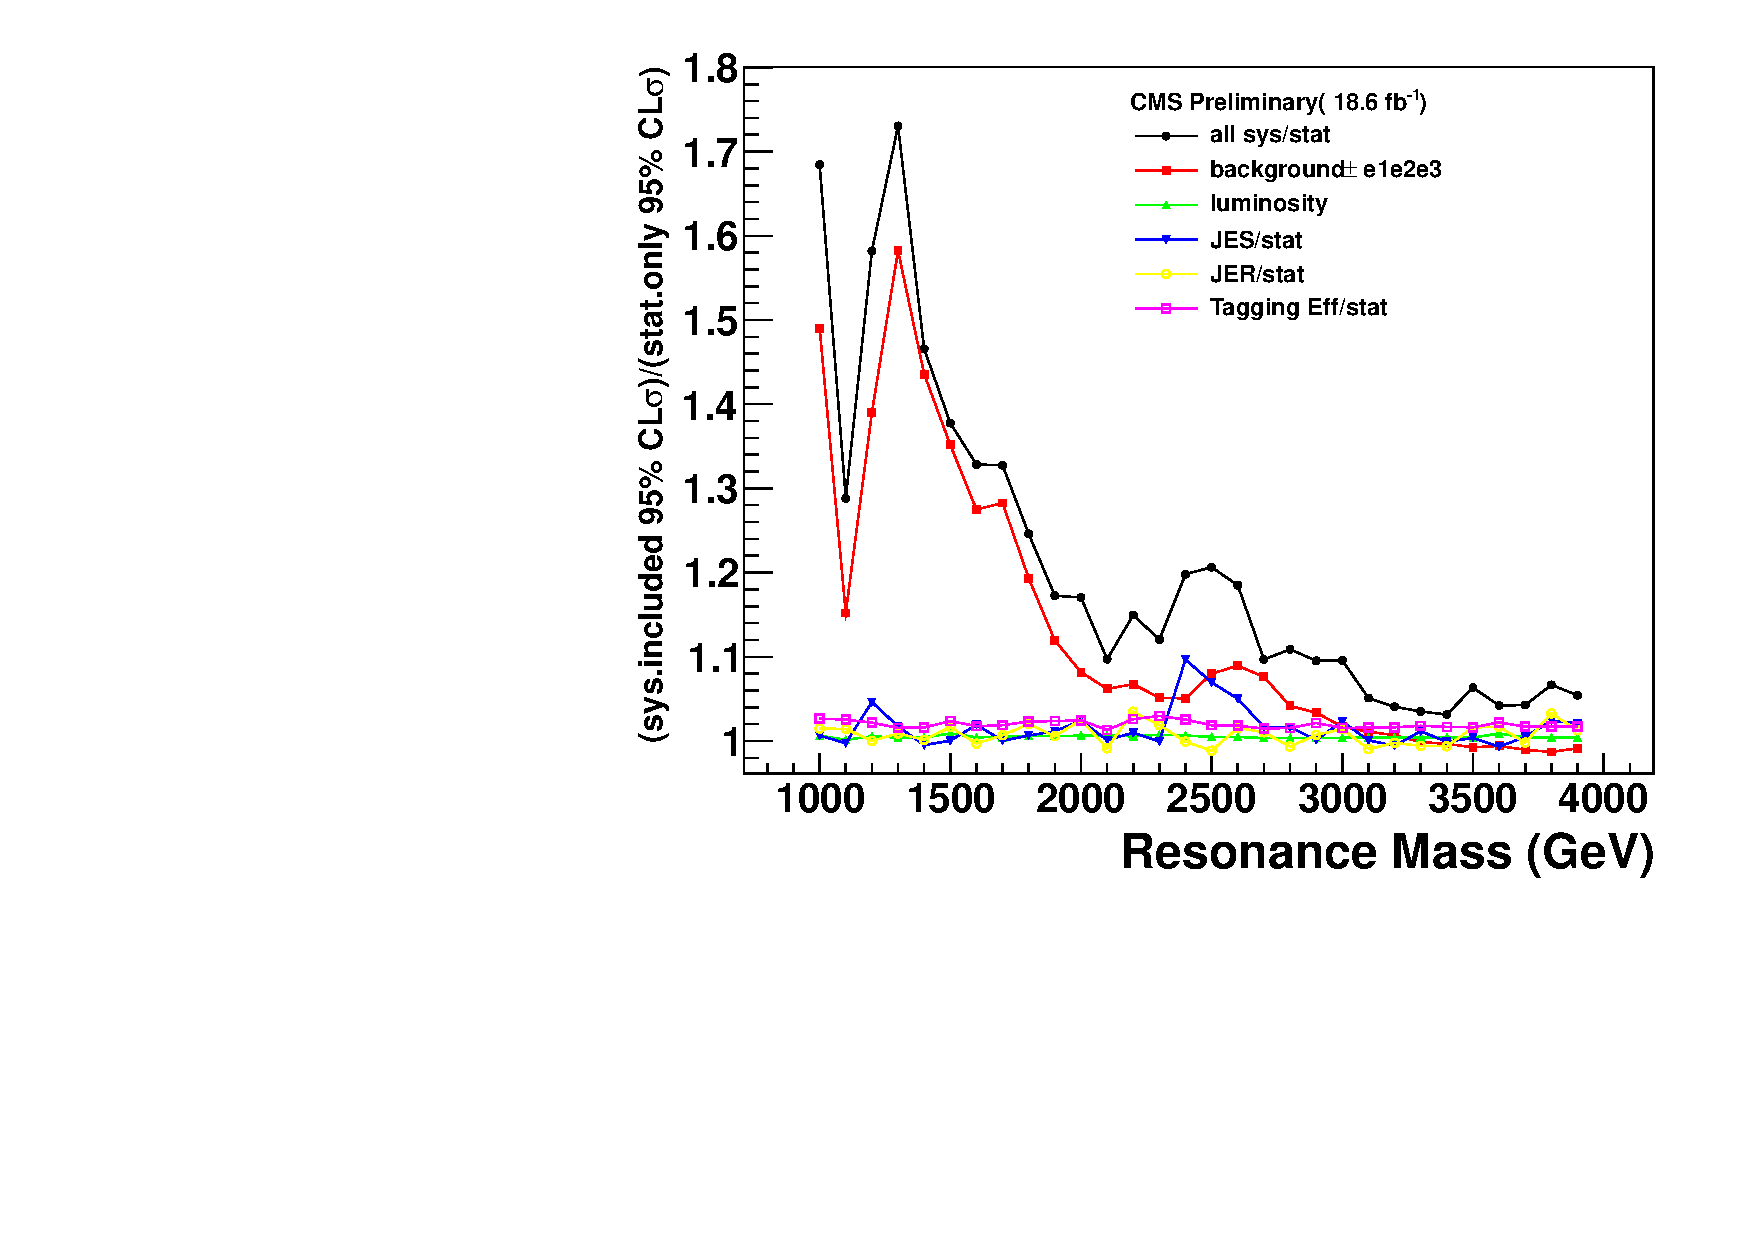
\includegraphics[width=0.48\textwidth,angle=0]{figs/single-Vtag-limits/qw-uncertainty.pdf}
%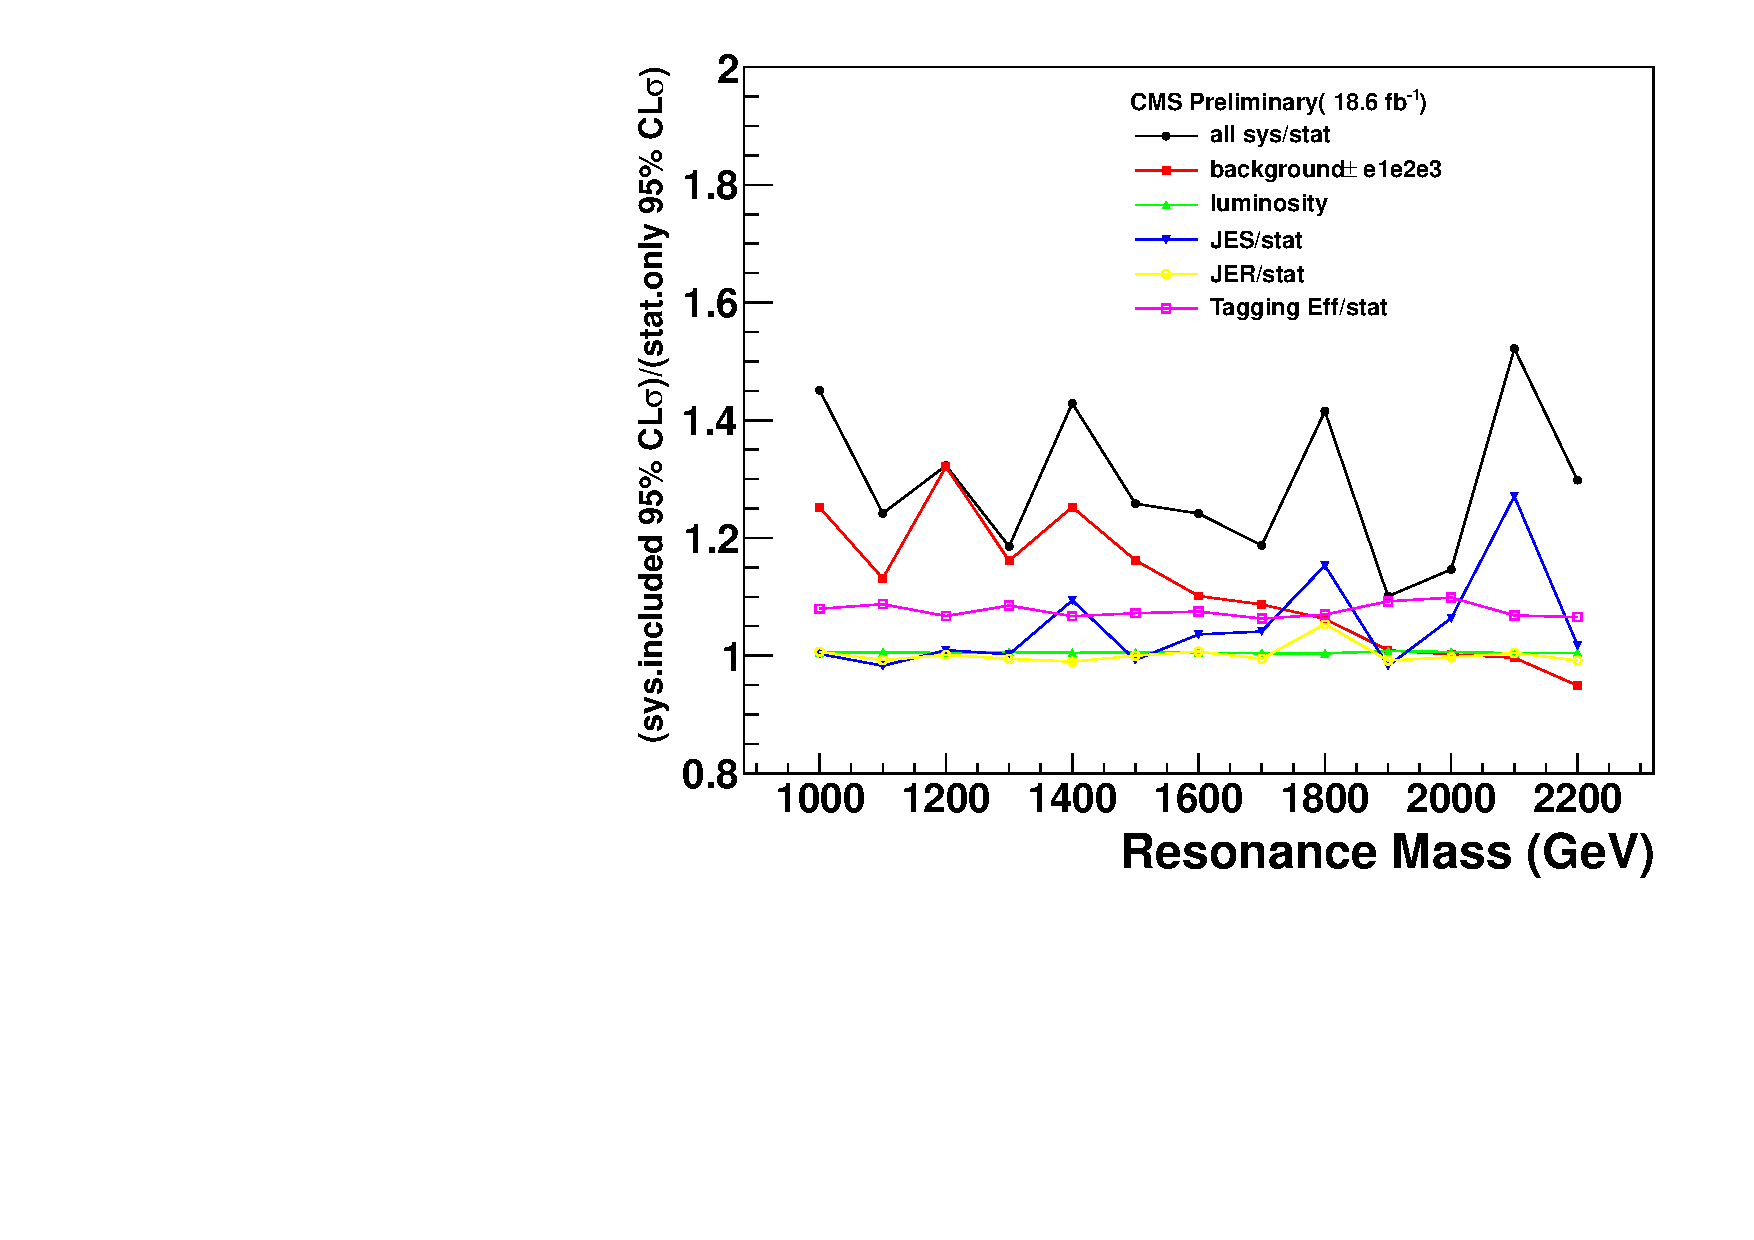
\includegraphics[width=0.48\textwidth,angle=0]{figs/double-Vtag-limits/ww-uncertainty.pdf}
%\end{center}
%\caption{Impact of the sources of systematic uncertainties on the observed limit with single (left) and double (right) W/Z-tag.}
%\label{fig:sysonlimit}
%\end{figure}

%The impact of the sources of systemtic uncertainties taken into account is demonstrated in Fig.~\ref{fig:sysonlimit}.
%The observed limit with each source of systemtic uncertainty is divided by the observed limit with statistical uncertainty only.
%The leading systematic uncertainty is the background uncertainty which increases the upper limit on the cross section by up to 80\%.



\clearpage
